%\chapter{面向拜占庭容错的隐私保护梯度聚合技术}
%\chapter{面向拜占庭容错的隐私保护联邦学习方案}\label{pbfl}
\chapter{面向拜占庭容错的模型参数安全聚合技术}\label{pbfl}
针对经典联邦学习直接交换模型参数导致的隐私泄露风险,同时兼顾拜占庭节点对全局模型造成的安全威胁,本章权衡了用户模型参数的隐私性、对拜占庭节点的鲁棒性以及聚合计算的高效性,提出了一种高效的面向拜占庭容错的隐私保护联邦学习方案(Privacy-preserving Byzantine-robust Federated Learning,PBFL)。

\section{引言}
%联邦学习(Federated Learning, FL)是目前主流的注重参与方数据隐私的分布式机器学习框架\cite{kairouz2019advances},它允许参与方不直接泄露本地数据的前提下,在联邦学习服务提供商的协调下,完成联合全局模型的训练。
%正是由于这种对原始数据的隐私保护,联邦学习实现了一定程度上的数据可用不可见,也被许多企业在实际应用中落地。
%比如谷歌使用联邦学习打造了针对移动端用户的联合输入法预测系统\cite{hard2018federated},可以给用户提供更加精准的输入词推荐;微众银行基于联邦学习部署了用户风险预测系统,更好的服务于对用户的风险评估服务。
%粗略地说,联邦学习主要有以下三个核心步骤:$(\rm \romannumeral1)$ 联邦学习服务提供商首先初始化随机的全局模型参数,然后分发给各个参与方;$(\rm \romannumeral2)$ 参与方收到全局模型参数后,将参数应用到本地,再使用本地数据集进行训练,更新本地参数,最后把更新后的参数(或梯度)上传给联邦学习服务提供商;$(\rm \romannumeral3)$ 服务提供商接收到符合条件的参数数量之后,对参数进行聚合,生成新一轮的全局模型参数。
%以上三个步骤一直被重复,直到联合训练的全局模型收敛。

虽然联邦学习避免了对用户数据的直接访问,但相关文献\cite{kairouz2019advances, mothukuri2021survey, geiping2020inverting} 指出联邦学习仍然面临着隐私和安全威胁,最典型的是针对用户模型参数对用户数据进行反向推理的推理攻击 \cite{geiping2020inverting},以及可以操控参与方上传恶意模型参数的拜占庭攻击\cite{kairouz2019advances, mothukuri2021survey}。

(1)推理攻击:攻击的敌对方是不诚实的联邦学习服务提供商,在接收到用户上传的参数之后,文献\cite{geiping2020inverting}指出联邦学习提供商可以根据用户上传的模型参数信息,反推出用户的隐私数据,这种攻击方式的存在意味着经典联邦学习直接上传参数的方式,不能完全保证用户的数据隐私,需要引入进一步的隐私增强策略来保证用户隐私。%TODO Details

(2)拜占庭攻击:攻击的敌对方是可以操纵参与方的敌手 $\mathcal{A}$,在用户进行本地训练以及参数上传的阶段,敌手$\mathcal{A}$可以通过刻意构造所上传的参数,达到扰动或者控制全局模型收敛方向,或者侵犯其它参与方数据隐私的目的\cite{kairouz2019advances}。值得注意的是,文献\cite{blanchard2017machine}指出尽管只有一个参与方被敌手$\mathcal{A}$所控制,也能破坏整个联邦学习全局模型的收敛方向。

正是由于上述攻击行为对现有联邦学习方案的隐私性和安全性提出的挑战,所以一个安全可信的联邦学习系统,需要同时做到:$(\rm \romannumeral1)$进一步保护用户模型参数的隐私,避免隐私数据被服务提供商窃取;$(\rm \romannumeral2)$保证服务提供商聚合参数时的鲁棒性,剔除恶意参数的影响。
要同时实现这两个目标,需要面对棘手的挑战。一方面,对恶意参数的识别与剔除往往需要对模型参数的直接访问;另一方面,对模型参数的隐私保护需求则需要对参数进行加密或者混淆。

%一些前沿的提升联邦学习拜占庭鲁棒性的方案\cite{blanchard2017machine, guerraoui2018hidden, yin2018byzantine}都假设聚合服务器是完全可信的,换言之,它不会从上传的用户模型参数中推断任何用户的隐私数据信息。
%因此,这些方案都直接让用户上传原始的模型参数,在明文上构建拜占庭鲁棒的聚合方案。例如,Krum\cite{blanchard2017machine}基于用户模型参数在欧氏空间的相似性实现了一定程度上的拜占庭鲁棒性,当上传的用户参数为明文时,计算效率尚可接受。但是在处理加密或者混淆过后的用户模型参数时,计算可行性和计算效率将成为方案的瓶颈。

%同时,也有一系列研究\cite{liu2021privacy, dong2021flod, nguyen2022flame, hao2021efficient, so2020byzantine}致力于同时实现模型参数的隐私保护以及聚合方案的拜占庭鲁棒性。
%PEFL\cite{liu2021privacy} 使用同态加密将用户本地梯度 $G_i$ 加密之后再上传到服务提供商,由两个半诚实非共谋的服务器完成鲁棒聚合,为了实现一些复杂密文计算,PEFL设计的四个安全计算协议都需要将 $\llbracket G_i\rrbracket_{pk}$ 使用随机数扰动之后,再进行解密操作。这里对于一个梯度 $G_i$ 的所有维度都使用相同的随机数进行扰动,会泄露梯度数据的数据分布信息,且相关研究\cite{comments}证明了利用PEFL泄露的分布信息,足以重构出用户的明文模型参数。FLOD \cite{dong2021flod} 和 SecureFL \cite{hao2021efficient} 方案都是基于FLTrust \cite{DBLP:conf/ndss/CaoF0G21} 的根数据集(Root dataset)思想,即服务提供商收集一小部分用户数据,用于判断和过滤恶意参数,显然这种方法会侵犯参与方的隐私。FLAME \cite{nguyen2022flame} 精心设计了拜占庭鲁棒聚合算法,并且结合ABY\cite{demmler2015aby} 以及隐私保护DBSCAN算法 \cite{bozdemir2021privacy} 实现了对用户梯度的隐私保护,但是其设计的鲁棒聚合算法涉及到安全两方计算(Secure 2-Party Computation,2PC)中开销较大的计算,其中包括梯度间余弦相似度的度量,以及共享份梯度的聚类操作,导致方案整体效率偏低。

%表\ref{cmp}在隐私性、鲁棒性和效率上对已有工作和本文的工作进行了粗略的对比。

针对以上安全与隐私威胁,本章首先提出了一个密文计算友好(即不涉及到开销较大的密文操作)的拜占庭鲁棒聚合算法,
再结合多方同态加密(Multiparty Homomorphic Encryption,MHE)技术为用户模型参数隐私提供强隐私保证,高效的在密文上剔除拜占庭参与方的影响。具体而言,本文的贡献如下:
\begin{compactenum}
	\item 提出了一个新颖的面向拜占庭容错的隐私保护联邦学习框架(PBFL),同时保证了用户模型参数的隐私和聚合后的全局模型参数的隐私。此外,PBFL还避免了研究工作\cite{liu2021privacy}中存在的梯度数据分布泄露的问题。
	\item 设计了一个高效的、密文计算友好的拜占庭鲁棒聚合算法,它以用户模型参数到上一轮全局参数欧式距离的中值为基准,动态调节参与方每轮聚合的权重,利用中值策略剔除恶意参数,充分发挥良性参数的作用。
	\item 对提出的方案在真实数据集上做了测试,实验结果表明PBFL可以有效的防御典型的拜占庭攻击,包括高斯攻击和标签转换攻击。此外,对方案进行了完备的安全性证明和收敛性证明,从理论上说明了方案可以在保护用户数据隐私的同时,实现对拜占庭节点的容错聚合。
\end{compactenum}

%\begin{table}[!h]
%	\centering
%	\caption{与类似方案在相关属性上的粗粒度对比}
%	\label{cmp}
%	 \scalebox{1.0}{
%		\renewcommand{\arraystretch}{1.2}
%		\begin{tabular}{l|cccc}
%			\toprule
%			% \hline
%			% \LEFTcircle \Circle \CIRCLE 
%			\textbf{提出的方案}               & \textbf{方法}      & \textbf{隐私}    &\textbf{鲁棒性} &\textbf{效率}              \\
%			\midrule
%			PEFL \cite{liu2021privacy}                   & 自定义聚合 + HE & \CIRCLE\Circle     &\CIRCLE\LEFTcircle     &\CIRCLE\LEFTcircle                       \\
%			FLAME \cite{nguyen2022flame}                   & 自定义聚合 + 2PC & \CIRCLE\CIRCLE     &\CIRCLE\LEFTcircle     &\LEFTcircle\Circle                       \\
%			FLOD \cite{dong2021flod}                   & FLTrust \cite{DBLP:conf/ndss/CaoF0G21} + 2PC & \CIRCLE\Circle     &\CIRCLE\CIRCLE     &\CIRCLE\LEFTcircle                       \\
%			SecureFL \cite{hao2021efficient}                   & FLTrust \cite{DBLP:conf/ndss/CaoF0G21} + 2PC & \CIRCLE\Circle     &\CIRCLE\CIRCLE     &\CIRCLE\LEFTcircle                       \\
%			本方案(PBFL)                   & 自定义密文计算友好聚合 + MHE & \CIRCLE\CIRCLE     &\CIRCLE\LEFTcircle     &\CIRCLE\CIRCLE                       \\
%			\bottomrule
%			% \hline
%		\end{tabular}
%		 }
%\end{table}

本章的组织结构如下:在第\ref{bg}节和第\ref{ps}节分别介绍了本章方案涉及到的一些预备知识和方案的问题描述;
然后在第\ref{friendly-alg}节和第\ref{PBFL}节对提出的面向拜占庭容错的模型参数安全聚合技术进行了细致的描述;接下来在第\ref{ana}节对方案进行了安全性分析、收敛性分析以及效率分析;在第\ref{eva}节对方案进行了实验评估;最后在第\ref{con}节对方案进行了总结。
%\newpage
\section{预备知识}\label{bg}

%\subsection{联邦学习}
%联邦学习(Federated Learning,FL)是目前前言的分布式机器学习方案,它可以让许多参与方(比如终端用户)在中央服务器的调度下,完成联合的机器学习或者深度学习训练,同时保证参与方数据留存在本地。在联邦学习中,中央服务器负责整个训练任务的初始化、以及训练过程中用户参数的聚合以及分发;而参与方负责使用本地数据优化收到的全局模型参数,然后将更新之后的参数上传给中央服务器。
%
%本方案的训练任务集中在经典的有监督学习任务,即图像分类的学习任务。
%具体来说,参与方 $P_i$ 持有本地隐私数据集 $D_i=\{(x_j, y_j);j=1,2,...,T\}$,其中$x_j\in\mathbb{R}^v$表示一个$v$维度的图像向量,而 $y_i$ 是该图像的真实标签。
%在训练轮次 $t$ 的开端,服务器会把全局参数 $W_g$ 分发给参与到训练的参与方,每个参与方 $P_i$ 将收到的全局参数 $W_g$ 应用到本地模型,然后使用本地数据集 $D_i$ 本地计算loss函数,计算方式如下:
%\begin{equation}
%	\mathcal{L}_f(D_i, W_g) \leftarrow\frac{1}{|D_i|}\sum\limits_{(x_j,y_j)\in D_i}\mathcal{L}_f(x_j,y_j,W_g),
%\end{equation}
%其中$\mathcal{L}_f(x_j,y_j,W_g)$是计算模型输出以及图像真实标签之间差异的loss值。
%联邦学习的目标是通过最小化全局loss函数的方式,获得最优的全局模型参数。
%在本方案中,我们利用随机梯度下降算法(stochastic gradient descent,SGD)来更新本地模型参数。
%即每个参与方对于$D_i$中的小批量数据$D_i^k \in D_i$,执行如下计算:
%\begin{equation}
%	W^{k+1}\leftarrow W^{k}-\eta\nabla\mathcal{L}_f(D_i^k,W^k)
%\end{equation}
%其中$k$代表本地训练周期。在本地参数更新完成之后,参与方$P_i$会获取到本轮更新的全局参数 $W_i^t$,然后将其发送给中央聚合服务器,等待服务器完成线性聚合:
%\begin{equation}
%	W_g^{t}\leftarrow\sum_{i=1}^{N}\frac{1}{N}W_i^{t},
%\end{equation}
%其中 $N$ 表示参与方的数量。参与方和服务器重复上述过程,直到全局模型收敛。

\subsection{拜占庭攻击}
在本章的拜占庭威胁模型中,敌手 $\mathcal{A}$ 可以控制一部分联邦学习参与方(拜占庭参与方)。
这些拜占庭参与方可以不向服务器发送更新的模型参数,而是发送任意的或精心构建的参数,来影响全局模型的准确率。
PBFL考虑了两种典型的非目标性的拜占庭攻击(Untargeted Byzantine Attack),即模型毒化攻击(Model Poisoning Attack)和数据毒化攻击(Data Poisoning Attack),具体描述如下:
\begin{compactitem}
	\item \textbf{模型毒化攻击:}这种攻击行为发生在本地用户的训练阶段,敌手 $\mathcal{A}$ 可以直接更改用户需要上传的模型参数,比如说可以胁迫参与方替换上传的参数为随机选取的高斯噪声,也被称为高斯攻击(Gaussian Attack,GA)\cite{blanchard2017machine, dong2021flod},GA攻击可以导致全局模型的大幅波动,从而严重影响全局模型的收敛。
	\item  \textbf{数据毒化攻击:}这种攻击通常发生在参与方数据的收集阶段,敌手$\mathcal{A}$ 可以修改用户收集到的本地数据,将数据的真实标签修改为错误的虚拟标签。以一张手写数字图片为例,其真实内容和标签都是5,而敌手$\mathcal{A}$可以保持图像数据特征不变,将标签改为9,从而影响全局模型的准确率,这种具体的攻击也被称为标签转换攻击(Label-Flipping Attack,LFA)\cite{kairouz2019advances, dong2021flod, liu2021privacy}。这种攻击可以破坏全局模型收敛的方向,从而大幅降低全局模型的准确率。
\end{compactitem}

\subsection{多方同态加密}
本文的隐私保护计算模块基于的是一种全同态加密(Cheon-Kim-Kim-Song,CKKS\cite{cheon2017homomorphic})的修订方案,即多方同态加密(Multiparty Homomorphic Encryption,MHE\cite{mouchet2020multiparty})。
在MHE中,可以由多个参与方本地持有私钥,在不泄露本地私钥的前提下,协同生成一份公钥。
而密文的解密操作则需要所有私钥持有方一起完成。
选择使用MHE构建PBFL的理由如下:
$(\rm \romannumeral1)$ 原生支持浮点数计算,非常契合神经网络模型参数以浮点数为主的场景。
$(\rm \romannumeral2)$ 基于环上的困难问题(Ring Learning with Errors,RLWE)搭建,可以实现抗量子攻击(Post-quantum Attacks)。
$(\rm \romannumeral3)$ 密文上的计算可以做到灵活且非交互。
$(\rm \romannumeral4)$ 支持安全的协同公钥切换操作,即在不解密一个密文的前提下,完成对密文的重加密(即用给定的另一份公钥加密),接下来对MHE方案进行简单介绍。

在MHE中,分圆多项式环的次数表示为 $\mathcal{N}$(取值为2的整数次方),决定了MHE的明文和密文空间分别为$R_{Q_{L}}=\mathbb{Z}_{Q_{L}}[X]/(X^{\mathcal{N}}+1)$和$Q_{L}=\prod_{0}^{L}q_i$,其中 $q_i$ 表示特定的素数,$Q_L$ 是初始等级为 $L$ 的密文模数。
图\ref{f1}中简单介绍了使用到的MHE相关函数。在图中,使用$\llbracket c\rrbracket_{pk}=(c_0,c_1)\in R^2_{Q_{L}}$ 和 $\overline{p}\in R_{Q_{L}}$ 分别表示MHE公钥加密后的密文和编码之后的明文。
%其它的符号描述可以参考\ref{tab:symbol}。
%我们分别使用 $L_c$, $S_c$, $L$, $S$ 表示
%TODO 这里的MHE概念加一点自己的理解
%TODO 描述改成脚注
%SUb
%POWER -> Mult -> rel
%InnerSum -> rotL/R + add
%Add
%MultByConst 
% 考虑用圈圈起来的符号,表示密文运算,
%  加法减法、求和简单来
图\ref{f1}中以$‘\textbf{D}’$开头的函数都是分布式的,需要由所有私钥持有方协同完成计算,而其它的函数在任意一方本地计算即可。

%\begin{table}[htbp]
%	\centering
%	\caption{MHE相关函数描述的符号标注}
%	\label{tab:symbol}
%	\begin{minipage}[t]{0.6\linewidth}
%		\begin{tabular*}{\linewidth}{lp{10cm}}
%			\toprule
%			符号 & 描述\\
%			\midrule
%			$L_c$ & 密文$\llbracket c\rrbracket_{pk}$当前的密文等级 \\ 
%			$S_c$ & 密文$\llbracket c\rrbracket_{pk}$当前的缩放量\footnote{缩放量是指密文解密后的明文和真实表示的明文之间的固定倍数关系} \\
%			$L$ & 密文的初始化等级\\
%			$S$ & 密文的初始化缩放量\\
%			\bottomrule
%		\end{tabular*}
%	\end{minipage}
%\end{table}

\begin{figure}[htb]
	\begin{framed}
		{\wuhao 
		\noindent \textbf{SecKeyGen($1^\lambda$):} 根据安全参数$ \lambda $返回私钥集合 ${sk_i}$,
		即对于参与方$P_i$来说. 本地生成私钥$ sk_i $。\\
		\noindent \textbf{DKeyGen(${sk_i}$):} 返回私钥持有方合作生成的公钥 $pk$。\\
		\noindent \textbf{DRelinKeyGen(${sk_i}$):} 返回协作生成的重线性化公钥 $rlk$。\\
		\noindent \textbf{DRotKeyGen(${sk_i}$):} 返回协作生成的元素位置旋转公钥 $rtk$.\\
		\noindent \textbf{Encode($msg$):} 将复数向量$msg$编码,返回明文多项式 $\overline{p}\in R_{Q_{L}}$,其缩放量$^*$为$S$。\\
		\noindent \textbf{Decode($\overline{p}$):} 对于明文多项式$\overline{p}\in R_{Q_{L}}$和对应的缩放量$S_{\overline{p}}$,返回解码之后的复数向量$\overline{p}$。\\
		\noindent \textbf{DDecrypt($\llbracket c\rrbracket_{pk}, {sk_i}$):} 对于密文 $\llbracket c\rrbracket_{pk}\in R^2_{Q_{L}}$ 和密文缩放量 $S_c$, 返回明文 $p\in R_{Q_{L}}$,其缩放量为$S_c$。\\
		\noindent \textbf{Enc($pk, \overline{p}$):} 返回密文 $\llbracket c\rrbracket_{pk}\in R_{Q_{L}}$ \\
		\noindent \textbf{Add($\llbracket c\rrbracket_{pk}, \llbracket c^{\prime}\rrbracket_{pk}$):} 返回 $(\llbracket c+c^{\prime}\rrbracket_{pk})$ 
		密文等级$^{**}$为min($L_c, L_{c^{\prime}}$), 缩放量为 max($S_c, S_{c^{\prime}}$).\\
		\noindent \textbf{Sub($\llbracket c\rrbracket_{pk}, \llbracket c^{\prime}\rrbracket_{pk}$):} 返回 $(\llbracket c-c^{\prime}\rrbracket_{pk})$ 
		密文等级为min($L_c, L_{c^{\prime}}$),缩放量为max($S_c, S_{c^{\prime}}$).\\
		\noindent $\textbf{Mul}_{ct}$$(\llbracket c\rrbracket_{pk}, \llbracket c^{\prime}\rrbracket_{pk})$: 返回 $\llbracket cc^{\prime}\rrbracket_{pk}$, 密文等级为min($L_c, l_{c^{\prime}}$),缩放量为($S_c\times S_{c^{\prime}}$).\\
		\noindent \textbf{Power}$(\llbracket c\rrbracket_{pk}, n)$: 返回 $\llbracket c^{n}\rrbracket_{pk}$,密文等级为 $(L_c-\log{n})$\\
		\noindent \textbf{RotL/R}($\llbracket c\rrbracket_{pk}, k$): 同态密文元素旋转操作(左移或者右移$k$次)。\\
		\noindent \textbf{DPubKeySwitch}$(\llbracket c\rrbracket_{pk}, pk^{\prime},{sk_i})$: 不解密的前提下,返回公钥切换后的密文$\llbracket c\rrbracket_{pk^{\prime}}$。\\
		\noindent $\textbf{MulByConst}(\llbracket c\rrbracket_{pk}, const)$: 返回密文$\llbracket c\times const\rrbracket_{pk}$,其缩放量取决于 $S_c$ 和 $const$,密文等级为$L_c$.\\
		% \noindent $\textbf{InnerSum}(\llbracket c\rrbracket_{pk}, batchSize, n)$: Returns $\llbracket c^{\prime}\rrbracket_{pk}$, the sum of $n$ sub-vector with $batchSize$ dimensions in vector hidden in $\llbracket c\rrbracket_{pk}$.
		\noindent $\textbf{InnerSum}(\llbracket c\rrbracket_{pk})$: 返回密文 $\llbracket c^{\prime}\rrbracket_{pk}$,解密后的第一个元素表示密文 $\llbracket c\rrbracket_{pk}$的内部元素和。}
		% \textbf{Our expansion, two sub-steps in DDecrypt:}\\
		% \textbf{1.PartDec}($\llbracket c\rrbracket_{pk},sk_i$): Returns a part of the decryption information $h_i$.\\
		% \textbf{2.AggDec}$(\llbracket c\rrbracket_{pk},\{h_i\})$: Returns the plaintext $p\in R_{Q_{L}}$ with scale $S_c$.
	\end{framed}
%	\begin{flushleft}
		\footnotesize
		*: 缩放量(Scale)表示当前值和所表达的真实值之间的固定倍数关系\\
		**:密文等级(Ciphertext level)取决于密文模数大小,决定了密文乘法操作的次数
%	\end{flushleft}
	\caption{MHE中常用的密文操作}
	\label{f1}
\end{figure}

%\newpage
\section{问题描述}\label{ps}

\subsection{系统模型}
PBFL的系统模型图如图\ref{syspnd}所示,其中主要有四个实体,具体描述如下:
\begin{compactitem}
	\item \textit{聚合服务服务提供商(Service Provider,SP):}SP为所有的联邦学习参与方提供协同训练的聚合服务。在每个联邦学习轮次中,SP收集用户上传的加密模型参数,聚合生成全局模型参数后分发给用户。
	\item \textit{计算服务器(Computing Server,CS):}CS负责辅助SP完成对用户上传的加密模型参数的聚合,即CS持有一份私钥,在不侵犯用户参数隐私的前提下,利用私钥计算SP需要的中间信息。
	\item \textit{数据拥有者(Data Owners,Parties in FL):}联邦学习中需要联合训练的参与方,在本地持有隐私数据。PBFL假定数据持有者可能被敌对方挟持,做出恶意行为扰乱联邦学习系统。
	\item \textit{密钥生成助手(Key Generation Assistant,KGA):}KGA协助所有参与方和SP生成用户侧的公私钥对,且保证参与方收到的私钥是同一份。为了避免KGA的独立解密行为,其和SP分别持有一份私钥,假设KGA是半诚实(semi-honest)实体且不和SP发生共谋行为,KGA在完成密钥生成之后,将持有的用户侧私钥安全的分发给所有参与方。
\end{compactitem}

\begin{figure}[htbp]
	\begin{center}
		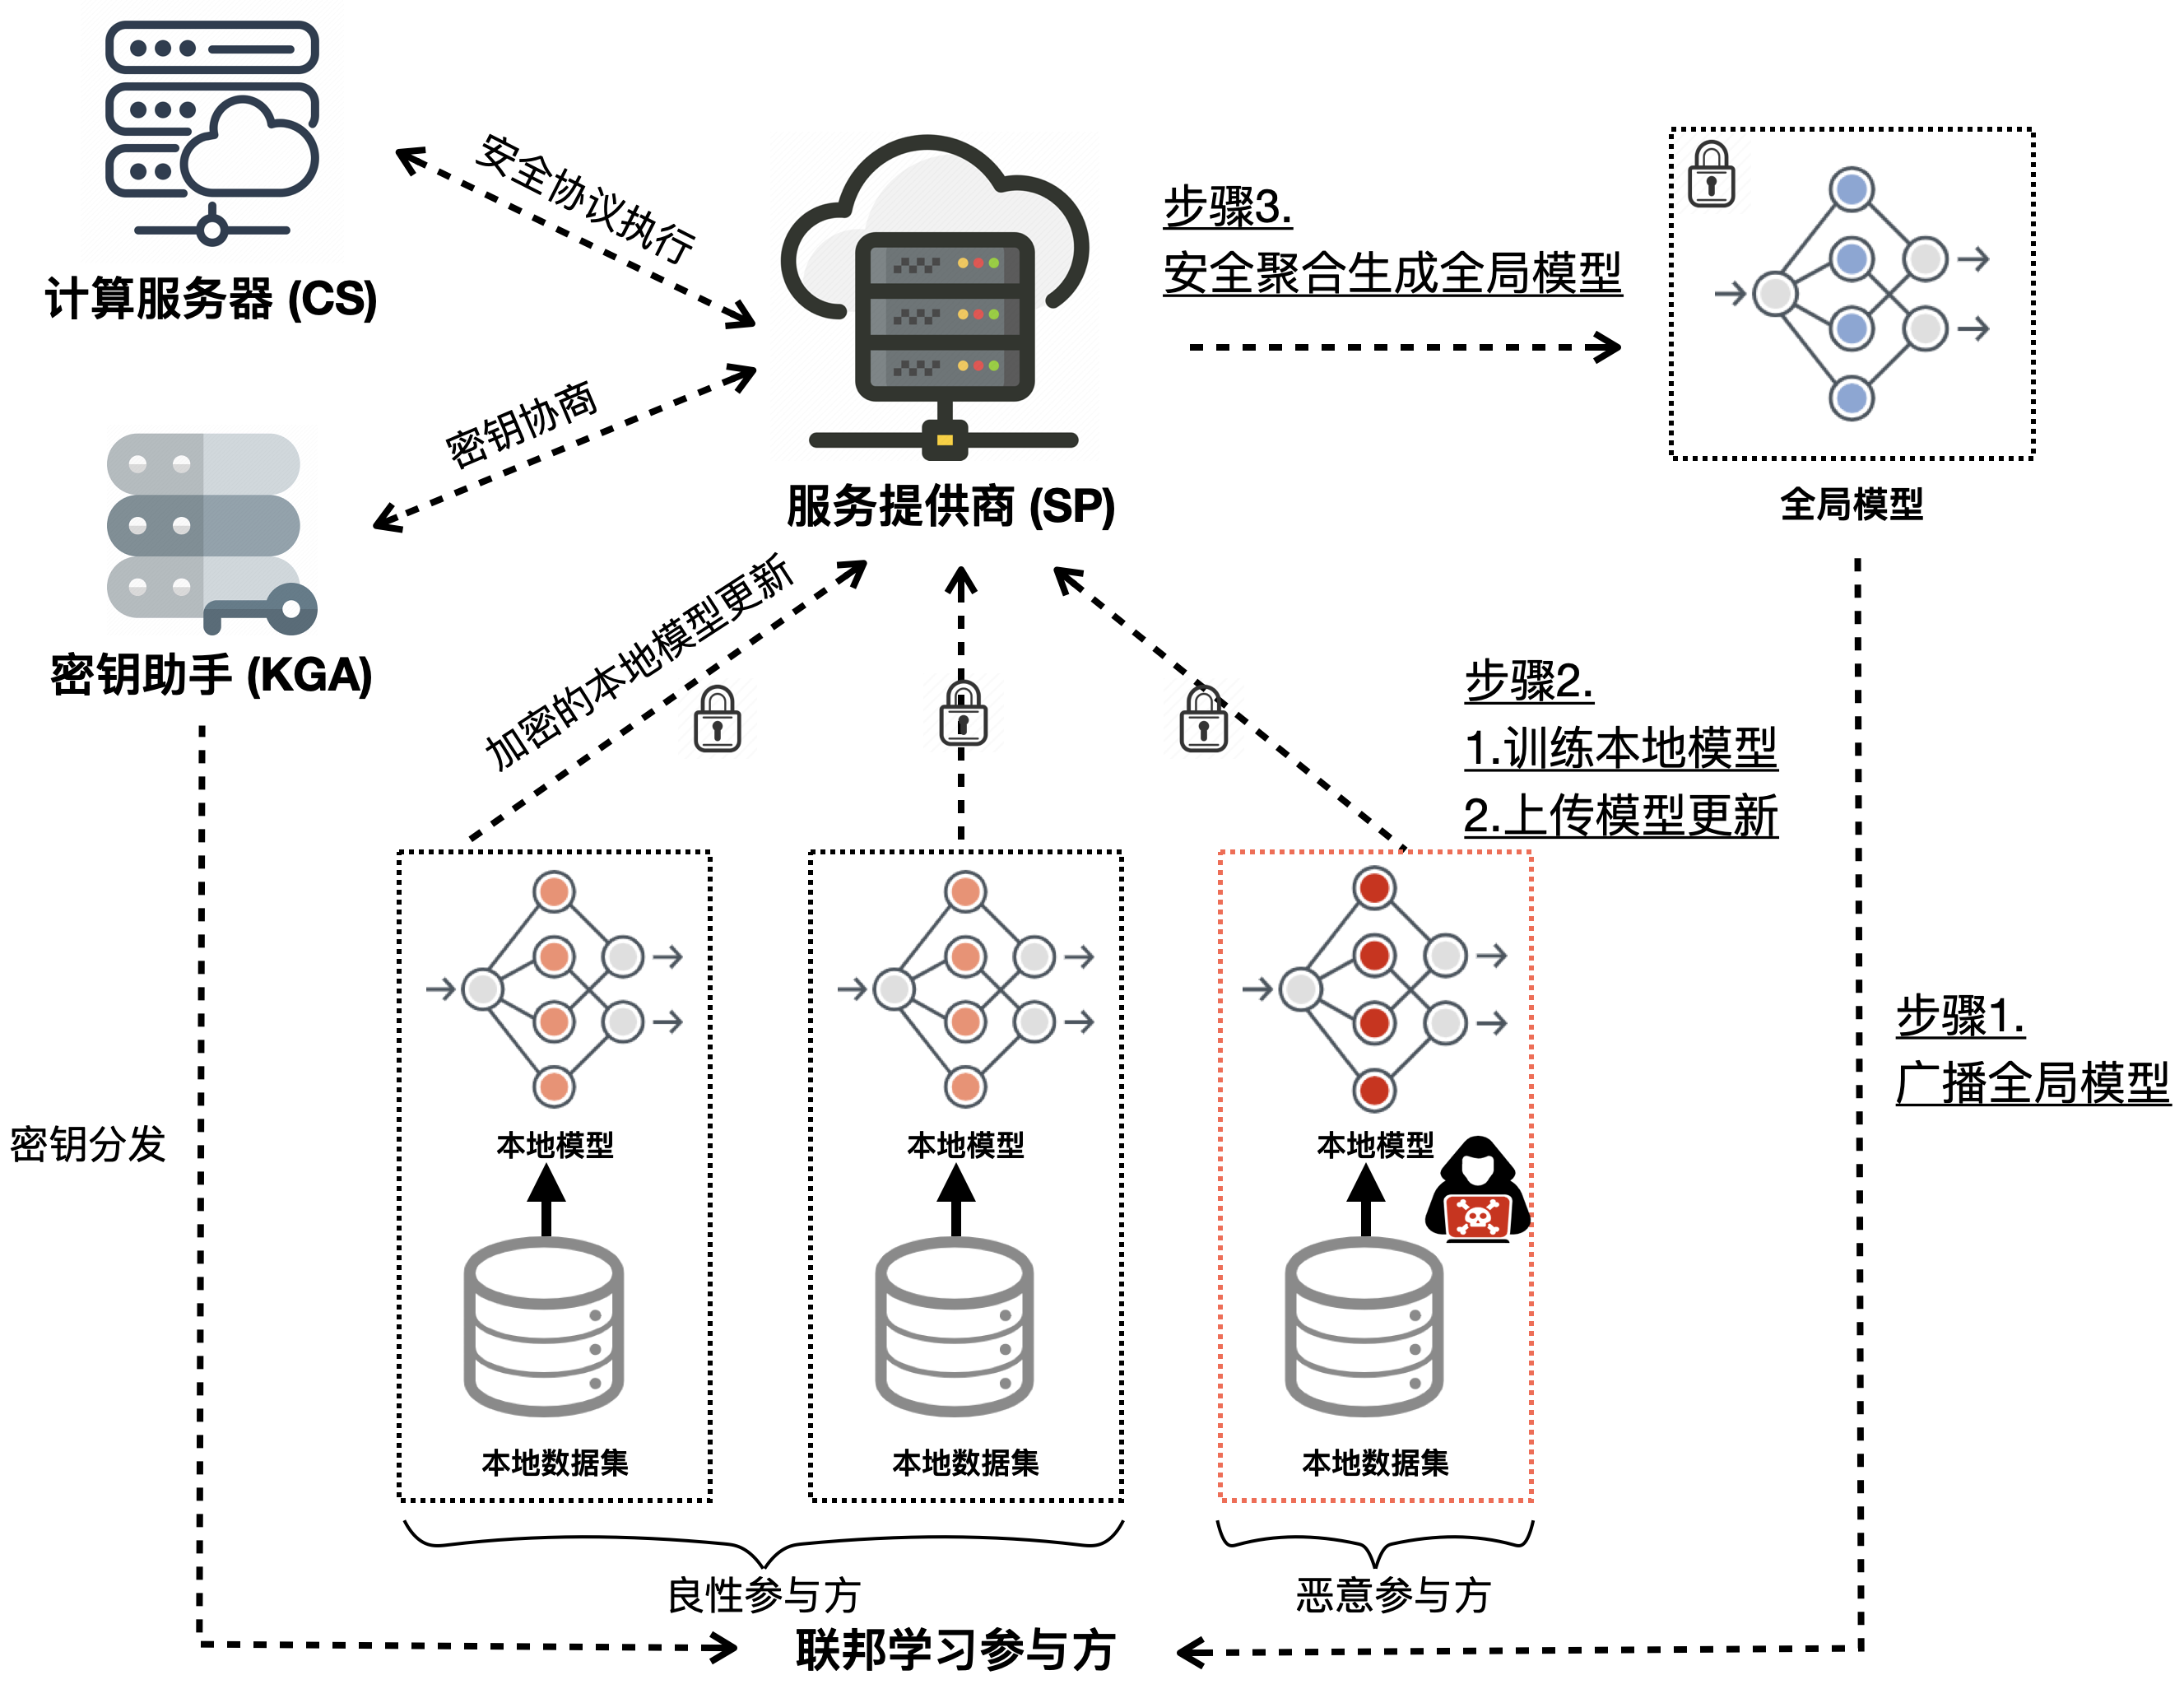
\includegraphics[width=0.8\linewidth]{figures/keynote-figs/PBFL.png}
		\caption{PBFL系统模型图}
		\label{syspnd}
	\end{center}
\end{figure}

\subsection{威胁模型}
PBFL旨在同时解决由半诚实聚合服务器造成的隐私威胁和由拜占庭参与方造成的安全威胁。假设联邦学习中的参与方的本地数据是独立同分布的(Independent Identically Distributed,IID)。
拜占庭参与方可以向SP发送任意的模型参数,从而影响全局模型的训练。
同时PBFL与类似工作\cite{so2020byzantine, yin2018byzantine, liu2021privacy}持有同样的假设,假定拜占庭参与方的上限不超过所有参与方的一半,即$|M|\leq\frac{|T|-1}{2}$,其中$|M|$ 和 $|T|$ 分别表示恶意参与方的数量和所有参与方的数量,这个假设是下文收敛性证明的前提。
除此之外,PBFL假设SP、CS和KGA是半诚实实体,这意味着它们将严格执行设计的安全协议,并且尝试从中推断出用户的隐私信息。
最后,假设方案中涉及到的四个实体SP、CS、KGA和持有数据的参与方,都不会和其它任意一方发生共谋行为。

\subsection{设计目标}
基于以上提到的系统模型和威胁模型,PBFL需要达到的目标如下:
\begin{compactitem}
	\item \textbf{保护模型参数隐私:}实现对用户上传的本地模型参数和聚合后的全局模型参数的隐私保护,保证模型参数对SP和CS而言,可用而不可见。
	\item \textbf{实现拜占庭容错:}对于可能出现的最多半数的拜占庭参与方,本方案将实现在密文上的拜占庭参与方过滤,保证全局模型的准确率。
	\item \textbf{提升全局模型准确率:}对比现有的其它方案,实现在相同恶意威胁模型下全局模型准确率的提升。
\end{compactitem}

\section{拜占庭鲁棒参数聚合算法}\label{friendly-alg}
本节详细描述设计的密文计算友好的拜占庭容错模型参数聚合算法。本章涉及到的符号在表\ref{sym}中进行了具体的描述。

为了设计密文计算友好的拜占庭容错参数聚合算法,本文提出了高效的距离计算基准选择以及有效的聚合权重赋予策略,详细描述如下:
\begin{compactitem}
	\item \textbf{高效的距离计算基准选择:}对用户本地模型参数进行评估时,需要一个基准(baseline)来判断用户参数的质量,即需要对比各方参数到基准参数的距离,决定参数的聚合权重(将权重赋予良性梯度)。笔者观察到,参与方的本地模型参数和上一轮的全局参数的距离,反映了用户本轮次更新的幅度大小,因此PBFL选择使用\textbf{上一轮的全局模型},作为距离计算的基准。这很好的提升了PBFL的密文友好性和计算复杂度,对比PEFL\cite{liu2021privacy}不需要进行复杂的参数基准计算(增加密文计算开销),即将基准的计算从复杂度$ O(N) $降低到了常数复杂度$ O(1) $,其中$N$表示参与方的数量。
	\item \textbf{基于中值的权重赋予策略:}针对选择的计算基准(上一轮的全局模型),拜占庭参与方可以从两方面进行攻击,$(\rm \romannumeral1)$进行幅度很小的更新或不更新,以此扰乱全局模型的收敛;$(\rm \romannumeral2)$进行幅度很大的更新,破坏全局模型参数更新的方向。因此,PBFL将到基准距离较小和较大的参数视为恶意参数,然后赋予较小甚至可忽略的聚合权重。而距离值位于中间的参与方被视为良性参与方,赋予较高的聚合权重。体现上述设计思路的具体算法如算法\ref{a0}所示。
\end{compactitem}
\begin{table}
	\centering
	\caption{符号说明}
	\label{sym}
	\scalebox{0.95}{
		\renewcommand{\arraystretch}{1.2}
		\begin{tabular}{cl}
			\toprule
			\textbf{符号}               & \textbf{描述}                      \\ 
			\midrule
			$\lambda$                      & 安全参数                        \\ 
			$pk_x$                         & 实体$x$的公钥                              \\ 
			$sk_x^y$                       & \makecell[l]{实体$y$持有的对应于公钥$ pk_x $的私钥份额} \\ 
			$D$                            & 用户本地数据                             \\ 
			$\mathtt{x}$                           & 数据样本特征                   \\ 
			$\mathtt{y}$                            & 数据样本标签                              \\ 
			$W_g$                            & 全局模型权重                            \\ 
			$W_i$                            & 用户$P_i$本地模型权重                             \\ 
			$G$                            & 模型梯度                           \\ 
			$\eta$                         & 模型训练学习率                          \\ 
			$N$                            & 联邦学习中参与方数量                 \\ 
			$\llbracket W \rrbracket_{pk}$ & 使用公钥$pk$加密的密文 \\ 
			$d$                            & 欧式距离平方           \\ 
			$f_s(P_x, t)$                  & \makecell[l]{在轮次t,表示计算出参与方$ P_x $聚合权重的抽象函数} \\
			$\gamma_i$                       & 参与方$P_i$的聚合权重       \\
			\bottomrule
		\end{tabular}
	}
\end{table}

\begin{algorithm}[htbp]
	\caption{密文计算友好的拜占庭鲁棒联邦学习聚合协议}
	\label{a0}
	\begin{algorithmic}[1]
		\REQUIRE 在轮次$t$,参与方本地模型参数 $\{W_1^t, W_2^t, ..., W_N^t\}$,其中$N$表示参与方数量,$W_g^{t-1}$ 表示上一轮的全局模型参数。
		\ENSURE 轮次$t$ 的全局模型参数 $W_g^t$。 
		\FOR{$i \in [1...N]$ 计算用户参数到基准的欧式距离平方}
		\STATE ${d}_i = \Vert W_i^t - W_g^{t-1} \Vert ^2$
		\ENDFOR
		\STATE 获取距离向量 ${d}$的中值:\\${d}_{mid} = median(\{{d}_{1}, {d}_{2},..., {d}_{n}\})$
		\FOR{$i\in[1...N]$ 计算到 $d_{mid}$ 的距离}
		\STATE $d^{\prime}_{i}=\left|d_i-d_{mid}\right|$
		% \STATE $d^{\prime}_{sum}=d^{\prime}_{sum}+d^{\prime}_{i}$
		\ENDFOR
		% \STATE Obtains the sum of the individual values in vector $d$ as $d_{sum}$
		\FOR{$i\in[1...N]$} %calculates the relative distance to $d_{mid}$}
	\STATE $scores_i=\dfrac{\sum_{j=1}^{N} (d^{\prime}_{j} + 1)}{d^{\prime}_i + 1}$ \COMMENT{距离$ d_{mid} $越近,聚合权重越高}
	\ENDFOR
	\FOR{$i\in [1...N]$ 缩放 $scores_i$ 到 0-1}
	\STATE $\gamma_i=\dfrac{scores_i}{\sum_{j=1}^{N} scores_j}$
	\ENDFOR
	\STATE 使用缩放后的权重线性聚合参数:\\
	$W_g^{t} =\sum_{i=1}^{N}\gamma_i * W_i^{t}$
\end{algorithmic}
\end{algorithm}

\section{拜占庭鲁棒的隐私保护联邦学习方案}\label{PBFL}
本节详细描述了PBFL如何赋予上述拜占庭鲁棒聚合算法完全的模型参数隐私保护能力。
粗略的说,首先参与方将使用MHE加密后的本地模型参数上传到SP,然后SP在CS的协助下,
在密文上确定每份本地模型参数的聚合权重,聚合完成后再完成全局参数的安全分发。总体上可以划分为四个阶段:系统初始化、本地模型训练、模型参数的安全聚合以及聚合模型参数的安全分发。

\subsection{系统初始化}
本阶段需要完成两对非对称密钥的生成与分发,
%包括服务端侧密钥集合和用户侧密钥集合,分别用于上传参数时对用户模型参数的加密和分发参数时对全局模型参数的加密。
首先SP和CS协同生成服务端侧密钥(下标以$ s $注明),其协同调用四个MHE安全协议SecKeyGen($\cdot$), DKeyGen($\cdot$), DRelinKeyGen($\cdot$), 和 DRotKeyGen($\cdot$),协同生成一份密钥集合$$ \{pk_s, rlk_s, rtk_s, sk_{s}^{SP}, sk_{s}^{CS}\},$$其中私钥$ sk_{s}^{SP} $由SP持有,私钥$ sk_{s}^{CS} $由CS持有,其余密钥公开,$ pk_s $用于明文的加密,$ rlk_s $用于密文乘法后的重线性化,$ rtk_s $用于计算内部元素之和时的元素移动。

随后KGA和SP之间协同生成用户侧密钥(下标以$ u $注明),通过执行SecKeyGen($\cdot$) 和 DKeyGen($\cdot$)协议,生成密钥集合$\{pk_u, sk_{u}^{SP}, sk_{u}^{U}\}$,其中私钥$ sk_{u}^{SP} $由SP持有,私钥$ sk_{u}^{U} $ 由KGA生成,然后安全分发给所有用户(所有用户持有相同用户侧私钥$sk_{u}^{U}$)。在这个过程中,KGA充当一个中介,使得所有用户和SP协商得到一份公私钥集合。为了保证KGA不直接持有用户侧私钥,对用户隐私造成威胁,PBFL使SP和KGA同时持有私钥,同时假设SP和KGA之间不发生共谋行为。

具体的私钥分配示意图如图\ref{keypng}所示。服务器侧公钥$pk_s$用于加密用户上传的模型参数,将私钥$\{sk_{s}^{SP}, sk_{s}^{CS}\}$分布于SP和CS之间为了保证SP不能直接解密用户上传的加密参数;而用户侧的公钥$pk_u$用于加密聚合后的全局模型参数,将私钥$\{sk_{u}^{SP}, sk_{u}^{U}\}$分布于SP和所有用户之间,是为了保证SP或者CS不能直接解密聚合后的模型参数。以此PBFL实现了本地模型参数和聚合后全局模型参数对SP和CS的完全保密。

\begin{figure}[htbp]
	\begin{center}
		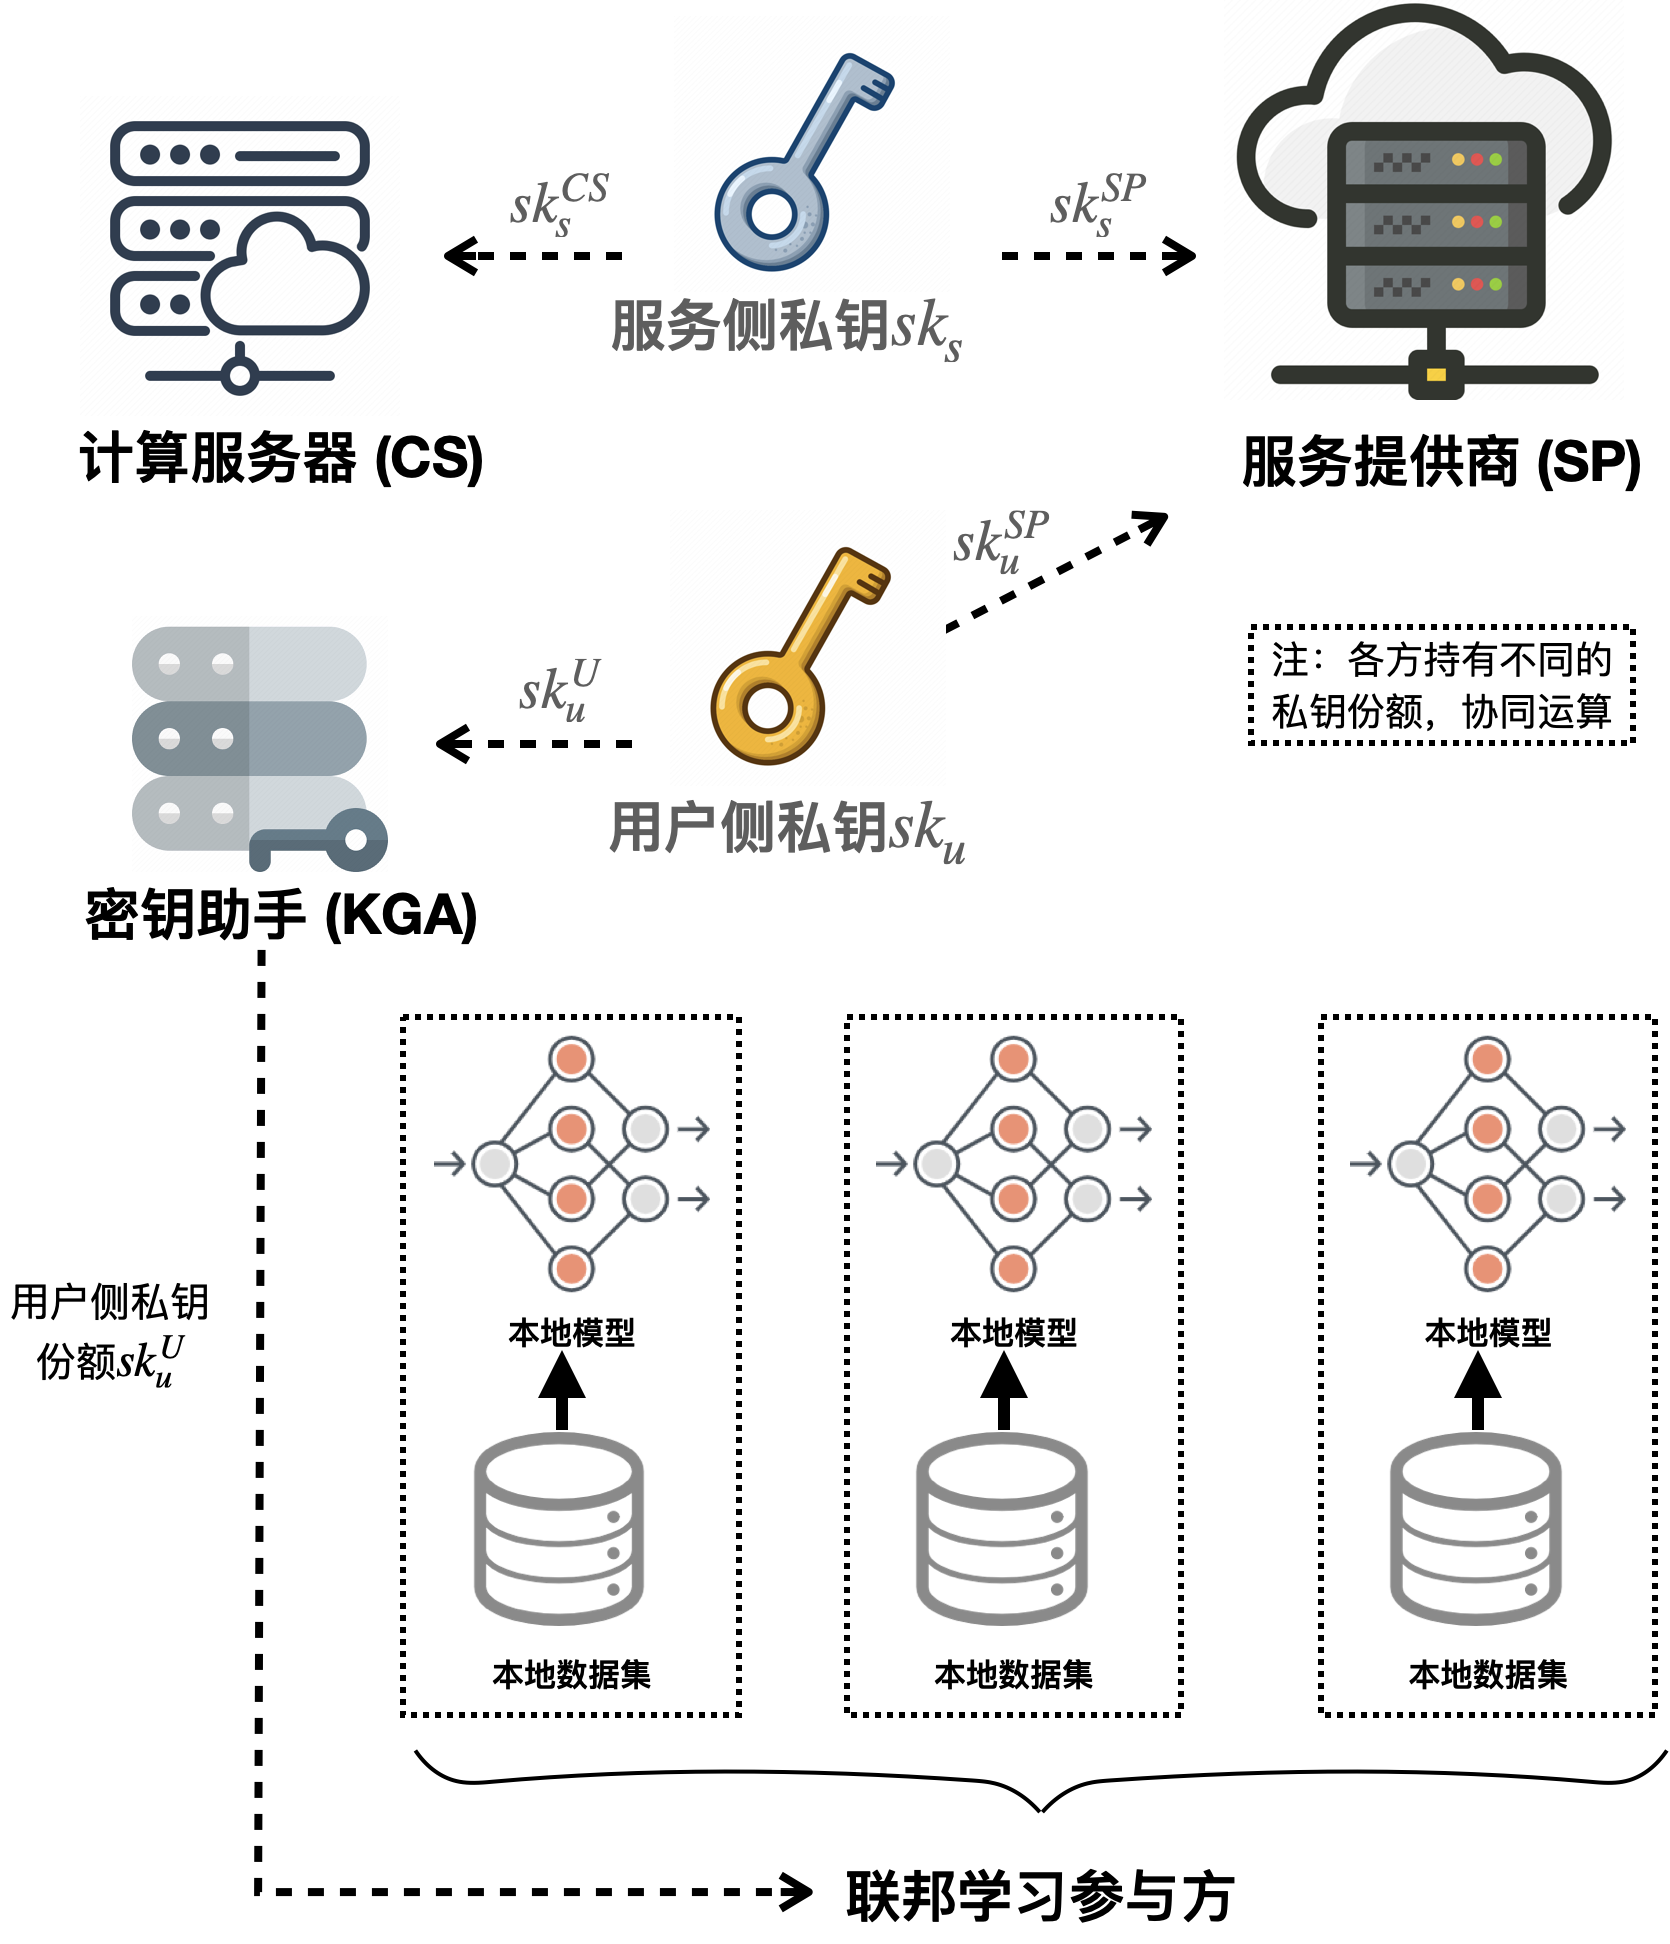
\includegraphics[width=0.5\linewidth]{figures/keynote-figs/Key-分配.png}
		\caption{私钥分布示意图}
		\label{keypng}
	\end{center}
\end{figure}

从密钥分配方案可知,PBFL的私钥皆由两方持有,于是本小节对MHE进行了两方安全计算协议的设计,其中包括安全的两方协同解密算法(Secure 2-party cooperative decryption,\textbf{Sec2Dec})和安全的两方协同公钥切换算法(Secure 2-party cooperative public key switch,\textbf{Sec2KeyS})。
\textbf{Sec2Dec}和\textbf{Sec2KeyS}以如下两个MHE分布式函数为基础:
\begin{compactitem}
	\item \textbf{DDecrpted($\cdot$)}:联合所有私钥持有方解密密文 $\ctx[pk]{c}$。以两方$P_1, P_2$ 分别持有私钥 $sk_1, sk_2$ 为例,为了解密密文 $\ctx[pk]{c}$,$P_1$ 和 $P_2$ 在本地分别利用私钥计算本地部分解密结果 $ h_1 $ 和 $ h_2 $,然后由一方收集所有本地解密结果,聚合得到密文的解密结果。这个分布式解密过程,可以做到对聚合方之外的另一方保密。为了方便描述,将这两个子过程分别命名为部分解密计算 PartDec$(\cdot)$ 和解密结果聚合 AggDec$(\cdot)$。
	\item  \textbf{DPubKeySwitch($ \cdot $)}:联合所有私钥持有方在不解密密文的前提下,对密文进行加密公钥的切换。同样以两方$P_1, P_2$ 分别持有私钥 $sk_1, sk_2$ 为例,为了将密文$ \ctx[pk]{c} $切换为由公钥 $ \ctx[pk^{\prime}]{c} $加密,$ P_1,P_2 $在本地利用私钥进行部分的公钥切换运算,然后再交由一方聚合所有的本地运算结果。整个分布式公钥切换的过程,不会泄露原始明文。为了简化描述,将两个子步骤命名为部分公钥切换计算PartSwitch($\cdot$) 和切换结果聚合AggSwitch($\cdot$)。
\end{compactitem}

具体的子步骤描述如图\ref{f2}所示。
\begin{figure}
	\begin{framed}
		{\wuhao
		\textbf{DDecrypt($\cdot$)}子步骤:\\
		\indent\textbf{1.PartDec}($\llbracket c\rrbracket_{pk},sk_i$): 返回本地部分解密信息 $h_i$。\\
		\indent\textbf{2.AggDec}$(\llbracket c\rrbracket_{pk},\{h_i\})$: 聚合各方部分解密信息$\{h_i\}$,返回明文 $c\in R_{Q_{L}}$。\\
		
		\textbf{DPubKeySwitch($ \cdot $)}子步骤:\\
		\indent\textbf{1.PartSwitch}($\llbracket c\rrbracket_{pk},{sk_i},pk^{\prime}$): 返回本地部分公钥切换信息 $s_i$.\\
		\indent\textbf{2.AggSwitch}$(\{s_p\})$: 联合各方部分公钥切换信息$\{s_p\}$,返回以新公钥$ pk^{\prime} $加密的密文 $\llbracket c^{\prime}\rrbracket_{pk^{\prime}} \in R^2_{Q_{L}}$。}
	\end{framed}
	\caption{MHE分布式函数步骤划分}
	\label{f2}
\end{figure}

\textbf{Sec2Dec}是MHE中分布式协同解密算法\textbf{DDecrypt($\cdot$)}在两方场景下的定制化。具体来说,PBFL对两方持有密文,需要另一方协同解密但又不向另一方泄露明文的场景,进行了协议设计。
假设私钥持有方$P_1,P_2$分别持有\footnote{$P_1,P_2$可以是方案实体中的任意两方,比如SP与CS,或SP与用户}私钥$sk^1, sk^2$,其对应公钥为$ pk $,$ P_1 $和$P_2$持有密文$\ctx[pk]{c}$,需要在对$P_2$保密的前提下,解密$\ctx[pk]{c}$,算法的细节描述如算法\ref{a-1}所示。
\begin{algorithm}[htbp]
	\caption{安全两方协同解密算法\\ \textbf{Sec2Dec}($\{sk^1, sk^2\}, \llbracket c\rrbracket_{pk}$) $\rightarrow c$}
	\label{a-1}
	\begin{algorithmic}[1]
		\REQUIRE 对于MHE密钥集合$(\{sk^1, sk^2\}, pk)$,私钥持有方 $P_1$ 和 $P_2$ 分别持有 $sk^1$ 和 $sk^2$;$P_1, P_2$ 持有密文 $\llbracket c\rrbracket_{pk}$.
		\ENSURE 私钥持有方 $P_1$ 获取明文 $c$, 且 $c$ 对$ P_2 $保密。
%		\IF{参与方 $P_2$ 不持有 $\llbracket c\rrbracket_{pk}$}
%		\STATE $P_1$ 发送 $\llbracket c\rrbracket_{pk}$ 给 $P_2$.
%		\ENDIF
		\FOR{$x \in \{1, 2\}$}
		\STATE 私钥持有方 $P_x$ 计算部分解密信息如下:\\ $\llbracket c_x\rrbracket_{pk} \leftarrow \textbf{PartDec}(\llbracket c\rrbracket_{pk}, sk^x)$. 
		\ENDFOR
		\STATE 私钥持有方 $P_2$ 发送 $\llbracket c_2\rrbracket_{pk}$ 到 $P_1$。
		\STATE 私钥持有方 $P_1$ 聚合部分解密信息如下:\\ $c \leftarrow \textbf{AggDec}(\llbracket c\rrbracket_{pk}, \{\llbracket c_1\rrbracket_{pk}, \llbracket c_2\rrbracket_{pk}\})$
		\RETURN $P_1$ 获取明文 $ c $.
	\end{algorithmic}
\end{algorithm}

\textbf{Sec2KeyS}是MHE中分布式公钥切换算法\textbf{DPubKeySwitch($ \cdot $)}在两方场景的定制化。具体来说,两个私钥持有方都持有密文,协议在两方不解密的前提下,完成对密文公钥的切换。
假设两个私钥持有方$P_1, P_2$分别持有私钥$sk^1, sk^2$,其对应公钥为$ pk_1 $,
同时$P_1, P_2$持有密文$ \ctx[pk_1]{c} $,想要将密文切换为由$ pk_2 $加密,即在对两方保密的前提下,获取密文$ \ctx[pk_2]{c} $,算法的细节描述如算法\ref{a-2}所示。

\begin{algorithm}[htbp]
	\caption{安全两方协同公钥切换算法\\ \textbf{Sec2KeyS}($\{sk^1, sk^2\}, pk_1, pk_2, \llbracket c\rrbracket_{pk_1})$ $\rightarrow \llbracket c\rrbracket_{pk_2}$}
	\label{a-2}
	\begin{algorithmic}[1]
		\REQUIRE 对于MHE密钥集合 $(\{sk^1, sk^2\}, pk_1)$, 私钥持有方 $P_1$ 和 $P_2$ 分别持有 $sk^1$ 和 $sk^2$;$P_1, P_2$ 同时持有密文 $\llbracket c\rrbracket_{pk_1}$;$pk_2$ 是密文 $\llbracket c\rrbracket_{pk_1}$ 公钥切换的目标公钥。
		\ENSURE 私钥持有方 $P_1$ 获得由公钥$pk_2$加密的密文$\llbracket c\rrbracket_{pk_2}$ ,且明文 $c$ 对 $P_1$ 和 $P_2$ 完全保密。
%		\IF{party $P_2$ does not hold $\llbracket c\rrbracket_{pk}$}
%		\STATE Party $P_1$ sends $\llbracket c\rrbracket_{pk_1}$ to party $P_2$.
%		\ENDIF
		\FOR{$x \in \{1, 2\}$}
		\STATE  私钥持有方$P_x$ 计算本地部分公钥切换信息:\\ $\llbracket c_x\rrbracket_{pk_2} \leftarrow \textbf{PartSwitch}(\llbracket c\rrbracket_{pk_1}, sk^x, pk_2)$
		\ENDFOR
		\STATE 私钥持有方 $P_2$ 发送 $\llbracket c_2\rrbracket_{pk_2}$ 到 $P_1$。
		\STATE 私钥持有方 $P_1$ 聚合公钥切换信息如下:\\ $\llbracket c\rrbracket_{pk_2} \leftarrow \textbf{AggSwitch}(\{\llbracket c_1\rrbracket_{pk_2}, \llbracket c_2\rrbracket_{pk_2} \})$
		\RETURN $ P_1 $ 获得密文 $\llbracket c\rrbracket_{pk_2}$, 且 $c$ 对 $ P_1, P_2 $完全保密。
	\end{algorithmic}
\end{algorithm}

\subsection{本地模型训练}
本阶段不需要提前知晓拜占庭参与方的真实占比,只假定其占比上限不超过$50\%$,对比需要以拜占庭节点比例作为先验知识的鲁棒聚合方案,即Krum\cite{blanchard2017machine}和Bulyan\cite{guerraoui2018hidden},本章方案PBFL更加切合实际场景。	

在训练的初始化阶段,SP将由用户侧公钥$ pk_u $加密的本轮全局模型参数
$ \ctx[pk_u]{W_g} $发送给所有参与本轮训练的用户。如上文所述,用户侧私钥$\{sk_u^{U}, sk_u^{SP}\}$由参与方$P_i$和$SP$分别持有,然后让这两个私钥持有方协同调用安全两方协同解密算法\ref{a-1}:
\begin{equation}\label{dec}
	W_g \leftarrow \textbf{Sec2Dec}(\{sk_u^U, sk_u^{SP}\}, \llbracket W_g\rrbracket_{pk_u})
\end{equation}
让$ P_i $获取到全局模型明文$ W_g $的同时,对SP保密。
紧接着参与方将全局模型参数$ W_g $应用到本地模型,使用本地数据集
$ D_i $进行训练,获取更新后的本地模型参数。具体而言,参与方$P_i$ 将数据样本特征$\mathtt{x}$输入到本地模型,获取到输出之后与标签$ y $计算交叉熵损失函数,然后再利用反向传播算法得到本次更新的梯度。
最后使用动量优化的随机梯度下降算法(SGD with momentum)更新本地模型参数。该方法同时考虑到了本次更新梯度和历史更新梯度,让参数的更新更加平滑。
在加速收敛的同时,减小了梯度的变化量,也让良性梯度之间相似度更高,更便于过滤恶意参数,不同类型的节点本地训练的步骤如算法\ref{a1}所示。

\begin{algorithm}[htbp]
	\caption{获取节点本地更新参数}
	\label{a1}
	\begin{algorithmic}[1]
		\REQUIRE 参与方 $P_i$的数据集 $D_i$,全局模型参数 $W_g$。
		\ENSURE $P_i$本地更新后的模型参数 $W_i$。
		\IF{$P_i$ 是 \textbf{GA拜占庭节点}}
		\STATE $W_i \leftarrow$ 正态分布随机向量采样
		\RETURN $P_i$ 的 $W_i$。
		\ELSE
		\STATE $\mathcal{B}\leftarrow$ 划分$D_i$为容量为$ B $的小批量数据
		\FOR {本地训练轮次 $i$ 从 $1$ 到 $E$}
		\FOR {批量数据 $b \in \mathcal{B}$}
		\IF{$P_i$ 是 \textbf{LFA拜占庭节点}}
		\STATE $label(b) \leftarrow 9-lable(b)$
		\ENDIF
		\STATE $G_{b}\leftarrow$ 计算$b$的梯度
		\STATE $W_i\leftarrow W_i - \eta G_{b}$
		\ENDFOR
		\ENDFOR
		\RETURN $P_i$的$W_i$。
		% \STATE $\llbracket W_i \rrbracket_{pk_u}\leftarrow$ Encrypt($W_i$, $pk_s$)
		\ENDIF
	\end{algorithmic}
\end{algorithm}

为了保护用户上传的模型参数隐私,用户$P_i$在获取到更新后的参数后,使用服务端侧公钥$ pk_s $对$ W_i $进行加密,得到 $ \ctx[pk_s]{W_i} $,然后发送给SP。通过使用MHE中的单指令多数据操作(Single Instruction Multiple Data,SIMD),可以将拥有较高维度的参数向量$W_i$打包进一个或者几个MHE密文,这极大的加速了后续安全聚合的进程。

\subsection{模型参数的安全聚合}
在本阶段,SP将在CS的协助下,完成对用户上传的加密参数的安全聚合。其中CS的协助步骤主要发生在两个阶段,第一个是部分信息的协助解密,第二个是聚合后密文从服务侧公钥$ pk_s $向用户侧公钥$pk_u$的安全切换。

对加密参数的安全聚合,首先要计算参数到基准的欧式距离平方,本方案选择的基准是上一轮的全局模型,所以对于聚合轮次$ t $来说,需要在密文上计算表达式$\left\| \llbracket W_i^{t} \rrbracket_{pk_s} - \llbracket W_g^{t-1} \rrbracket_{pk_s} \right\|_2^2$的值,其中$ \llbracket W_i^{t} \rrbracket_{pk_s} $表示密文用户参数,$ \llbracket W_g^{t-1} \rrbracket_{pk_s} $表示密文上一轮全局参数。
具体步骤如下:SP首先在密文上计算$\textbf{Sub}(\cdot)$和$ \textbf{Power}(\cdot) $函数,得到用户参数到基准的差值平方,最后执行$ \textbf{InnerSum}(\cdot) $函数求和所有内部元素的和,得到的密文即包含了所需的欧式距离平方信息,为了解密这个信息,SP和CS协同调用安全两方协同解密算法\ref{a-1},在保证距离信息对CS完全保密的前提下,让SP获取明文的距离信息,算法的细节描述如算法\ref{a2}所示。

\begin{algorithm}[htbp]
	\caption{安全欧式距离平方计算\\ \textbf{SecDis}$(\llbracket W_i^{t}\rrbracket, \llbracket W_g^{t-1}\rrbracket)\rightarrow d_i$}
	\label{a2}
	\begin{algorithmic}
		\REQUIRE 在轮次$t$, SP 持有第 $t-1$ 轮 全局模型参数$\llbracket W_g^{t-1} \rrbracket_{pk_s}$以及参与方$P_i$的本地模型参数 $\llbracket W_i^{t} \rrbracket_{pk_s}$;SP 和 CS 分别持有 $sk_{s}^{SP}$ 和 $sk_{s}^{CS}$,以及对应的服务侧公钥$pk_s$。
		\ENSURE $\llbracket W_i^{t}\rrbracket$ 和 $\llbracket W_g^{t-1}\rrbracket$之间的欧式距离平方。
	\end{algorithmic}
%	\textbf{Performed by SP and CS}\\
	\textbf{SP:}
	\begin{algorithmic}[1]
		\STATE 计算差值:\\$\llbracket tmp\rrbracket_{pk_s}\leftarrow {\textbf{Sub}}(\llbracket W_i^{t} \rrbracket_{pk_s}, \llbracket W_g^{t-1} \rrbracket_{pk_s})$
		\STATE 计算平方:\\$\llbracket tmp \rrbracket_{pk_s}\leftarrow {\textbf{Power}}(\llbracket tmp\rrbracket_{pk_s}, 2)$
		\STATE 计算内部元素和:\\$\llbracket d_i \rrbracket_{pk_s}\leftarrow {\textbf{InnerSum}}(\llbracket tmp \rrbracket_{pk_s})$
		% \STATE Sends $\llbracket W_{isum} \rrbracket_{pk_s}$ to SP.
	\end{algorithmic}
	\textbf{SP \& CS:}
	\begin{algorithmic}[1]
		\STATE SP 和 CS 协同解密: \\ $d_i \leftarrow \textbf{Sec2Dec}(\{sk_{s}^{SP}, sk_{s}^{CS}\}, \llbracket d_i \rrbracket_{pk_s})$
		% \STATE Calculates the partial decryption information: \\$hd_{CS}^{(t+1)}\leftarrow {\rm PartDec}(\llbracket W_{isum} \rrbracket_{pk_s}, sk_{s}^{CS})$
		% \STATE Sends $hd_{CS}^{(t+1)}$ to SP.
		\RETURN SP得到欧式距离平方$d_i$。
	\end{algorithmic}
\end{algorithm}

在获取到用户参数到基准的距离之后,接下来聚合权重的计算和算法\ref{a0}(第4-13行)一致,细节描述如下:

首先SP对所有参与方到基准的距离向量$\{d_1, d_2,...,d_N\}$进行排序,然后获取到中值,结果以$d_{mid}$表示。紧接着计算所有距离值到$ d_{mid} $的相对距离:
\begin{equation}\label{dToMid}
	d^{\prime}_{i}=\left|d_i-d_{mid}\right|
\end{equation}
得到距离向量$\{d^{\prime}_1, d^{\prime}_2,...,d^{\prime}_N\}$,根据所有的相对距离给每个参与聚合的密文参数打分,距离中值越近的得分越高,反之得分越低,计算方式如下:
\begin{equation}\label{sc}
	scores_i=\frac{\sum_{j=1}^{N} (d^{\prime}_{j} + 1)}{d^{\prime}_i + 1}
\end{equation}
在等式\ref{sc}中,本文以距离值$d^{\prime}_i + 1$作为分母\footnote{加一避免分母为0},然后以向量和作为分子,这意味着相对$d_{mid}$距离越小,计算出来的得分越高。换言之,距离$d_{mid}$越近的参数,得分越高,同时也将距离$d_{mid}$偏差大的用户(距离过小或过大的参数),赋予了更低的分数。将得分等比例缩放为聚合权重,计算方式如下:
\begin{equation}
	\gamma_i=\dfrac{scores_i}{\sum_{j=1}^{N} scores_j}
\end{equation}
最后使用得到的聚合权重$\gamma$对密文用户参数进行线性聚合:
\begin{equation}\label{e3}
	\llbracket W_g\rrbracket_{pk_s}=\sum_{i=1}^{N}\gamma_i*\llbracket W_i\rrbracket_{pk_s}
\end{equation}
其中$*$表示常数和密文的乘法,$\sum$表示多个密文的加法运算。

\subsection{聚合模型参数的安全分发}\label{broadcast-para}
本阶段完成对聚合后全局参数的分发,在上述步骤执行完成之后,SP得到了聚合后的全局模型参数$ \llbracket W_g\rrbracket_{pk_s} $,其结果被服务侧公钥$pk_s$所加密,无法被用户直接解密使用,所以需要在对SP以及CS保密的前提下,将加密公钥切换至用户侧公钥$pk_u$。
SP和CS对聚合后的全局参数密文执行安全两方公钥切换协议,可以达到以上目的。
具体来说,SP和CS分别持有服务侧私钥$\{sk_s^{SP}, sk_s^{CS}\}$,协同调用如下过程:
%\begin{small}
	\begin{equation}\label{e4}
		\begin{aligned}
			\llbracket W_g\rrbracket_{pk_u} \leftarrow \textbf{Sec2KeyS}(\{sk_s^{SP}, sk_s^{CS}\}, pk_u, pk_s, \llbracket W_g\rrbracket_{pk_s})
		\end{aligned}
	\end{equation}
%\end{small}
最后SP将得到由用户侧密钥加密的全局参数密文$\llbracket W_g\rrbracket_{pk_u}$,将其广播给所有参与方。

%\textbf{讨论:}PBFL中对用户参数和基准之间的欧式距离平方值进行了解密操作,本文认为这个操作不会侵犯到用户的数据隐私。首先很明显SP获取的一维距离信息,无法推导出模型中任何一个参数的具体信息,包括参数的大小、方向以及单个元素的正负。文献\cite{geiping2020inverting}提出的针对梯度的数据重构方案,可以根据梯度之间的余弦相似度,重构用户的训练样本,但是它需要知道梯度各个维度的正负信息,在PBFL中,SP无法获取这个信息,所以不会泄露用户的数据隐私。

\textbf{讨论:}PBFL中对用户参数和基准之间的欧式距离平方值进行了解密操作,本文认为这个操作不会侵犯到用户的数据隐私,理由如下:

现有的根据模型参数推理隐私数据的方法\cite{zhu2019deep, geiping2020inverting},核心思路是将模拟数据向量$\mathtt{x}$和标签$\mathtt{y}$输入全局模型,生成模拟梯度$g_i^{\prime}$,再以最小化模拟梯度$g_i^{\prime}$和真实梯度$g_i$之间的距离作为优化目标,迭代更新向量$\mathtt{x}$和标签$\mathtt{y}$。Zhu等人\cite{zhu2019deep}提出的DLG算法的优化目标是模拟梯度$g_i^{\prime}$和真实梯度$g_i$的欧式距离。Geiping等人\cite{geiping2020inverting}提出的梯度反转算法认为在重构数据时,梯度的方向(Direction)比梯度的大小(Magnitude)更加有效,因此使用模拟梯度$g_i^{\prime}$和真实梯度$g_i$的余弦相似度作为优化目标,在优化时可只利用真实梯度$g_i$中各维度的正负信息。综上可知,将梯度反转为隐私数据,需要获取全局模型参数(用于生成模拟梯度)和参与方本轮次的真实梯度信息(用于构造优化目标),显然本章对于欧式距离平方的解密操作,不会泄露参与方梯度的大小、方向以及各个维度的正负信息,同时,本章方案对于聚合后的全局模型也做到了对SP和CS保密(见参数分发阶段\ref{broadcast-para}),因此不会泄露用户的数据隐私。

\section{理论分析}\label{ana}
本节首先对PBFL进行了安全性和收敛性分析,最后对比分析了PBFL的效率表现。
\subsection{安全性分析}\label{sec-ana}
本小节证明方案对于用户模型参数和全局模型参数,做到了对半诚实服务器的完全保密。

CKKS同态加密方案的语义安全性(Semantic security)基于环上的LWE(Learning with Errors)难题,
实现了对于选择明文攻击、选择密文攻击以及中间人攻击等攻击方式的逐比特安全\cite{cheon2017homomorphic, lindner2011better, lyubashevsky2010ideal}。
%并且可以被Albrecht提出的LWE-Estimator所计算 \cite{albrecht2019homomorphic, albrecht2015concrete}。
MHE方案基于CKKS方案对多方协同计算做了拓展,方案涉及到的分布式密文计算协议,即DKeyGen($\cdot$),DPubKeySwitch($\cdot$), 和 DDecrypt($\cdot$),其安全性已被Mouchet等人证明 \cite{mouchet2020multiparty},保证了这些协议在被半诚实计算参与方执行时的安全性。本小节首先提出了如下命题,并且给出证明。
%真实视图和模拟视图不可区分
%涉及到许多的子协议,我们使用hybrid augment 混合论证方式来对整个协议的安全性进行论证。
%定义一个模拟器,行为是对REAL进行一些改造,改完之后发现计算无法区分。
\begin{proposition}[对半诚实服务器的安全性]\label{pro1}
	对于给定的安全参数$ \lambda $,联邦学习的参与方集合$\mathcal{U}$(包括用户$\{P_1, P_2,...,P_N\}$),以及联邦学习服务提供商集合$\mathcal{S} = \{SP, CS\}$,本节以随机变量$\mathcal{R} e a l_{\mathcal{S}}^{U, \lambda}$表示半诚实服务器集合$\mathcal{S}$在协议执行过程中获取的所有视图,存在一个概率多项式时间模拟器$\mathcal{SIM}$,其输出的模拟视图$ \mathcal{S I} \mathcal{M}_{\mathcal{S}}^{U, \lambda} $与真实视图$\mathcal{R} e a l_{\mathcal{S}}^{U, \lambda}$之间计算不可区分(Computationally Indistinguishable),即:
	$$
		\mathcal{S I} \mathcal{M}_{\mathcal{S}}^{U, \lambda} \stackrel{c}{\equiv} \mathcal{R} e a l_{\mathcal{S}}^{U, \lambda}
	$$,
	其中$\mathop{\equiv}\limits^{c}$表示计算不可区分。
\end{proposition}

\begin{proof}
	根据真实视图$\mathcal{R} e a l_{\mathcal{S}}^{U, \lambda}$的定义,其包含所有服务器集合$\mathcal{S}$在执行上诉协议的中间状态以及接收到的信息。本文采用标准的混合论证(hybrid argument)\cite{bonawitz2017practical, xu2020privacy}来证明命题\ref{pro1}。对于安全参数$ \lambda $,本文定义了概率多项式模拟器$\mathcal{SIM}$,其可以对真实视图 $\mathcal{R} e a l_{\mathcal{S}}^{U, \lambda}$中的随机变量进行一系列的修改,生成模拟视图$ \mathcal{S I} \mathcal{M}_{\mathcal{S}}^{U, \lambda} $,下面的混合论证集合可以说明,模拟视图$ \mathcal{S I} \mathcal{M}_{\mathcal{S}}^{U, \lambda} $和真实视图$\mathcal{R} e a l_{\mathcal{S}}^{U, \lambda}$之间具有计算不可区分性,细节描述如下所示。
\end{proof}

\begin{hybrid}\label{h1}
	本论证初始化一个与执行协议产生的真实视图$\mathcal{R} e a l_{\mathcal{S}}^{U, \lambda}$分布不可区分的模拟视图。
\end{hybrid}

\begin{hybrid}\label{h2}
	本论证模拟用户和SP之间的协同解密过程,即等式\ref{dec}的协同执行,让用户以随机变量$\ctx[pk_u]{\alpha_i}$替换本地部门解密结果$\ctx[pk_u]{c_i}$,其安全性由MHE中的DDecrypt($\cdot$)保证,所以本论证与论证\ref{h1}不可区分。
\end{hybrid}

\begin{hybrid}\label{h3}
	本论证改变模拟的用户集合$\mathcal{U}$中良性用户的参数加密上传行为,每个良性用户$P_i$加密一个随机采样的向量$\alpha_i$,而不是真实的用户模型参数$W_i$。这时只有上传的密文发生了变化,CKKS的语义安全性以及SP与CS之间的不共谋,保证了本论证和论证\ref{h2}不可区分。
\end{hybrid}

\begin{hybrid}\label{h4}
	本论证改变安全欧式距离计算\ref{a2}(SecDis)的输入,以加密的随机变量$\llbracket \alpha_{g}^{t-1}\rrbracket_{pk_s}$和$\llbracket \beta_i^{t}\rrbracket_{pk_s}$,替换原来的输入$\llbracket W_{g}^{t-1}\rrbracket_{pk_s}$和$\llbracket W_i^{t}\rrbracket_{pk_s}$。由于只有密文内容发生了改变,MHE的语义安全性和SP与CS之间不共谋的性质,保证了本论证和论证\ref{h3}不可区分。
\end{hybrid}

\begin{hybrid}\label{h5}
	本论证假设在安全欧式距离计算算法\ref{a2}中,SP向CS发送的是加密的随机变量$\llbracket \alpha_i\rrbracket_{pk_s}$,而不是计算所得的欧式距离平方$\llbracket d_i \rrbracket_{pk_s}$,其中$i \in [1...N]$。尽管CS持有公钥$pk_s$对应的两份私钥中的一份$sk_s^{CS}$,MHE的联合解密过程需要保证所有私钥持有方的参与,因此结合SP与CS不共谋的特性,可以保证CS无法完成解密,从而保证本论证和论证\ref{h4}不可区分。
\end{hybrid}

\begin{hybrid}\label{h6}
	本论证将SP执行的密文线性聚合等式\ref{e3}中的输入$\llbracket W_i\rrbracket_{pk_s}$修改为加密随机变量$\llbracket \alpha_i\rrbracket_{pk_s}$,计算结果的密文发生了改变,MHE的语义安全性以及服务器之间不共谋的性质,保证了此论证和论证\ref{h5}无法区分。
\end{hybrid}

\begin{hybrid}\label{h7}
	本论证改变SP和CS执行安全公钥切换算法时的输入,即执行等式\ref{e4}时的输入,以随机变量$\llbracket \alpha_g\rrbracket_{pk_s}$替换聚合后的全局模型参数$\llbracket W_g\rrbracket_{pk_s}$,此时也只有密文内容发生了变化,CKKS的语义安全性以及服务器之间的不共谋假设,保证了此论证和论证\ref{h6}不可区分。
\end{hybrid}

\begin{hybrid}\label{h8}
	本论证修改安全公钥切换算法的中间计算结果,即模拟CS计算得到随机变量$\beta_{CS}$,而不是部分公钥切换信息$c_{CS}$,其安全性由MHE中的DPubKeySwitch($\cdot$)保证,因此本论证和论证\ref{h7}不可区分。
\end{hybrid}

以上混合证明证明了存在一个概率多项式模拟器$ \mathcal{SIM} $可以按照上述方式生成模拟视图,并让其和真实视图在计算上做到不可区分,因此证明了半诚实的SP和CS在安全协议执行过程中,无法窃取用户的模型参数信息,进而确保用户的数据隐私。

%TODO 加一个用户无法侵犯用户隐私

\subsection{收敛性分析}
本节证明PBFL全局模型在有拜占庭参与方的前提下,依然能够收敛的性质,首先提出如下命题:
\begin{proposition}[误差项]\label{pro2}
	良性参与方生成的模型参数与拜占庭节点生成的模型参数之间存在一个误差项$\epsilon$,即满足以下等式:
	$$
		\sum_{u\in U}W_u=   \sum_{u\in B}W_u^{\kappa} + \epsilon	
	$$
	其中$U$和$ B $分别表示良性参与方集合以及拜占庭参与方集合。
\end{proposition}

\begin{proof}
	良性参与方集合的目标是联合训练得到目标模型参数$W^{\star}$,而拜占庭参与方的训练目标则是让全局模型向恶意目标$W^{\kappa}$发展。
	每一轮的模型参数取决于用户利用本地数据得到的梯度$G$,即在第$t$轮次,$W^{t} = W^{t-1} - \eta G$,其中$ \eta $是本地训练学习率。
	实现恶意攻击的方式是控制拜占庭节点,形成具有恶意目标的梯度$G^{\kappa}$,而良性节点得到梯度的方式是利用本地独立同分布的数据,生成梯度:
	$$
		G^{\star} \leftarrow \nabla_{W} \mathcal{L}_{f}(D,W)
	$$
	其中所有良性用户$G^{\star}$的期望$E[G^{\star}]=g$,$g$表示全局良性梯度的无偏估计。因此,良性梯度聚合得到的全局参数的期望$E[W^{\star}]$,也是全局良性模型参数$w$的无偏估计。由于恶意梯度$G^{\kappa}$的目标是扰乱良性梯度$G^{\star}$,所以这两者之间存在明显的差距$\tau$,$\tau = G^{\star}-G^{\kappa}$,因此可以得出参数之间也有明显的差距$W^{\kappa} = W^{\star} - \eta \tau$,所以可知:
	\begin{align*}
		\sum_{x\in B}W_x^{\kappa} & = \frac{|B|\sum_{x\in U}W_x^{\star}}{|U|} - |B|\eta\tau                                \\
		& = (\frac{|B|}{|U|}-1)\sum_{x\in U}W_x^{\star} + \sum_{x\in U}W_x^{\star} - |B|\eta\tau \\
		& = \sum_{x\in U}W_x^{\star} + (\frac{|B|}{|U|}-1)|U|w - |B|\eta\tau
	\end{align*}
	良性参数和恶意参数之间的误差项,因为其不同的目标而必然存在,即$\sum_{u\in U}W_u=   \sum_{u\in B}W_u^{\kappa} + \epsilon$,其中$ \epsilon = (\frac{|B|}{|U|}-1)|U|w - |B|\eta\tau $。
\end{proof}

基于以上误差项的存在,本文进一步给出全局模型收敛性的命题和证明:
\begin{proposition}[收敛性]
	在执行完一定轮次第\ref{friendly-alg}节和第\ref{PBFL}节中的安全鲁棒聚合方法后,全局模型将收敛至良性用户的目标模型参数。
\end{proposition}

\begin{proof}
	假设参与方$P_x$的聚合权重$\gamma_{x}$由一个抽象的函数$f_s(P_x,t)$决定,其中$t$表示当前训练轮次,$P_x$表示来着参与方集合$U$或者集合$B$的用户,其中$ U $表示良性用户集合,而$ B $表示拜占庭参与方集合。PBFL假设拜占庭参与方的比例上限为$50\%$,即$\abs{B} <\abs{U}$。全局模型的收敛性取决于是否由良性用户主导整个训练过程,即满足以下条件:
	\begin{equation*}
		\begin{split}
			\mbox{条件}\ 1:{\forall}P_x \in B, f_s(P_x,t)\rightarrow 0 \\
			\mbox{条件}\ 2:{\forall}P_x \in U, f_s(P_x,t)\rightarrow 1
		\end{split}
	\end{equation*}
	
	本文把$W_x^{\star}$假设为良性用户$P_x$的理想模型参数,根据命题\ref{pro2}可知,良性用户参数和恶性用户参数之家存在一个误差项:$\sum_{x\in U}W_x^{\star}=   \sum_{x\in B}W_x^{\kappa} + \epsilon$,利用到这个特性,PBFL的鲁棒聚合算法可以识别出与良性参数相距甚远的恶意参数,赋予其低至可忽略的聚合权重。
	当拜占庭参与方持续上传恶意的模型参数时,误差项$\epsilon$逐渐变大,赋予其的聚合权重逐渐接近于0,即对于拜占庭参与方$P_x \in B$,$f_s(P_x, t)\rightarrow 0$,这满足了条件1。因此良性用户的聚合权重满足:
	$$
		\lim_{t \to \infty}\sum_{x \in U} \gamma_x = 1
	$$
	这意味着良性用户聚合权重的和无限接近于1,满足了条件2。
	%在真实数据集上的实验结果如表\ref{t1}所示,也证明了本文命题的正确性。
	
	随着以上两个条件的满足,良性用户将逐渐主导整个联邦学习训练过程,最后实现全局模型的收敛目标。
\end{proof}

\subsection{效率分析}
本节对PBFL的运行效率进行分析,同时和类似方案进行了效率对比,以展现PBFL在效率上的优势。首先对安全计算协议计算开销进行分析,然后再对通信开销进行分析。

\subsubsection{计算开销分析}
在PBFL中,服务器侧的计算开销主要集中在安全的参数聚合以及分发阶段,此阶段服务器需要在密文上计算用户参数到基准的欧式距离平方,然后在密文上完成参数的聚合和分发。以下分析执行一轮协议,具体的开销情况。

假设参与方数量为$N$,其模型参数维度为$M$,首先分析安全欧式距离计算协议\ref{a2} \textbf{SecDis},对于其涉及到的五次密文简单线性操作,复杂度为$O(5*M)$,对于涉及到的内部元素求和协议\textbf{InnerSum($\cdot$)},其复杂度为$O(Mlog(M) + M)$,因此总的复杂度为$O(6*NM+NMlog(M))$。然后SP获取到了距离向量明文$d$(长度为$N$),与模型参数维度无关,所以后续权重的计算非常高效,复杂度为$O(Nlog(N) + 3*N)$,其中$O(Nlog(N))$表示对向量的取中值操作,$O(3*N)$代表三次简单的明文向量操作。
最后在聚合密文的公钥切换阶段,其中有三次简单密文线性操作,复杂度为$ O(3*M) $。
对于用户侧的计算开销,主要随着模型参数的维度$M$和数据样本数量$s$的增长而增长,复杂度为$O(Ms)$。

\subsubsection{通信开销分析}
在PBFL中,服务器侧的通信开销主要集中在两个阶段,第一个是欧式距离计算阶段,CS协助解密距离信息,第二个是聚合后密文的公钥切换阶段,需要私钥持有方SP和CS联合完成公钥的切换。
在第一阶段,对于$N$个用户,SP需要发送$N$个密文给CS,其中每个密文包含维度为$M$的参数向量,通信复杂度可以表示为$O(NM)$,然后CS完成对所有用户距离信息的部分解密信息计算,发送给SP,其通信复杂度也为$O(NM)$。
在第二个阶段,SP需要将聚合后的密文发送给CS,通信开销为$O(M)$,然后CS将计算结果发送给SP,通信复杂度为$O(M)$。
综上所述,SP和CS之间仅进行了两个轮次的通信,并且每轮次通信的通信量都不大。

为了展示PBFL在效率上的优势,本小节逐协议比较了类似工作\cite{liu2021privacy}和本方案之间的开销差异,结果如表\ref{cmp2liu}所,可以看到PBFL在计算和通信开销上都有一定优势,其中服务器间通信开销优势明显。

同时,本小节对PBFL和前沿工作在不同属性上进行了对比,具体如表\ref{detail-cmp}所示,可以看出PBFL在权衡用户数据隐私、对拜占庭节点的容错以及计算效率上更加出色。

\begin{table*}
	\centering
	\caption{与文献\parencite{liu2021privacy}在计算和通信开销上的对比}
	\label{cmp2liu}
	 \scalebox{0.9}{
		\renewcommand{\arraystretch}{1.2}
		\begin{tabular}{c|c|c|c}
			\toprule
			% \hline
			% \LEFTcircle \Circle \CIRCLE 
			\textbf{提出的方案}               &\textbf{阶段 \#}      & \textbf{计算开销复杂度}           & \textbf{通信开销复杂度}             \\
			\midrule
			\multirow{4}{*}{PEFL \cite{liu2021privacy}}& 1 &$O(NMlog(N))$ &$O(NM+M)$\\
			& 2 & $O(5*NM)$ &$O(2*NM+N)$ \\
			& 3 & $O(6*NM)$ &$O(2*NM)$ \\
			& 4& $O(4*M)$ &$O(2*M)$  \\
			% \hline
			% \multirow{4}{*}{Our PBFL} 
			\hline
			\multirow{4}{*}{本方案(PBFL)}& 1 &$O(5*NM + NMlog(M)))$ &$O(2*NM)$\\
			& 2 & $O(Nlog(N)+3*N)$ & - \\
			& 3 & $O(3*M)$ &$O(2*M)$ \\
			% & 4& $O(4*M)$ &$O(2*M)$  \\
			% Our PBFL                                & $O(5*NM + NMlog(M))) + O(Nlog(N)+3*N) + O(3*M)$                           & $O(2*NM) +  O(2*M)$ \\
			\bottomrule
			% \hline
		\end{tabular}
		 }
\end{table*}


% \footnote{FLTrust based schemes requires root data from users, which violates user privacy}

\begin{table*}
	\centering
	\caption{与现有方案在特定属性上的粗粒度比较}
	\label{detail-cmp}
	 \scalebox{0.9}{
	 			\renewcommand{\arraystretch}{1.2}
	 	\begin{tabular}{l|ccccc}
	 		\toprule
	 		% \hline
	 		% \LEFTcircle \Circle \CIRCLE 
	 		\textbf{提出的方案}                & \makecell[c]{\textbf{不持有根数据集}\\ \textbf{(Root Data)}}    &\makecell[c]{\textbf{本地模型}\\ \textbf{隐私保护}} &\makecell[c]{\textbf{全局模型}\\ \textbf{隐私保护}} & \makecell[c]{\textbf{计算开销和}\\ \textbf{通信开销}} & \makecell[c]{\textbf{拜占庭}\\ \textbf{鲁棒性}}             \\
	 		\midrule
	 		PEFL \cite{liu2021privacy}                   & \ding{51} & \ding{51}     &\ding{51}     & 中   & 中                    \\
	 		FLAME \cite{nguyen2022flame}                   & \ding{51} & \ding{51}     &\ding{55}     & 高   & 中 $\sim$ 高            \\
	 		FLOD \cite{dong2021flod}                   & \ding{55} & \ding{51}     &\ding{55}     & 高     & 高                 \\
	 		SecureFL \cite{hao2021efficient}                   & \ding{55} & \ding{51}     &\ding{55}     & 中  & 高                      \\
	 		本方案(PBFL)                   & \ding{51} & \ding{51}     &\ding{51}     &低     & 中                  \\
	 		\bottomrule
	 		% \hline
	 	\end{tabular}
 	}
\end{table*}

\section{实验评估}\label{eva}
本节在真实数据集上做了一系列的实验,以此证明方案在提升联邦学习隐私性的同时,保证了对拜占庭节点的鲁棒性。
本节所有的实验都在一台配置有Ubuntu 20.04, Intel(R) Core(TM) i9-10980XE CPU @ 3.00GHz CPU 和 64GB RAM 的主机上进行,其中参与方和服务器分别用不同的进程来模拟。
实验中神经网络训练部分使用PyTorch实现,服务侧安全聚合中的同态运算部分使用Lattigo\cite{lattigo}实现,两者之间的通信使用gRPC实现。

\subsection{实验初始化}
本节主要从两个角度来评估方案的性能,第一个是方案提出的聚合算法在全局模型上的准确率表现;第二个是面对典型非目标性拜占庭攻击的鲁棒性。为了展示PBFL的优越性,本节复现了四种典型的联邦学习模型参数聚合方案进行对比分析,分别是FedAvg,Krum,Median 和 Trimmed Mean方案。

\subsection{攻击描述}
PBFL的设计目标是同时防御来自半诚实服务器的推理攻击和来自拜占庭节点的拜占庭攻击。其中对于DLG等典型的利用梯度重构数据的推理攻击\cite{zhu2019deep, geiping2020inverting},PBFL通过基于MHE的安全协议设计实现了对用户模型参数和聚合后全局模型参数的强隐私保护(安全协议设计见第\ref{PBFL}节,安全性分析见第\ref{sec-ana}节),此类攻击方式无法获取模型梯度或者权重进行攻击,因此本节不对此类攻击进行实验评估。

本节的实验主要模拟了两种典型的非目标性拜占庭攻击:高斯噪声攻击(Gaussian attack,GA)和标签反转攻击(Label-flipping attack,LFA)。
为了模拟GA的攻击场景,被敌对方$\mathcal{A}$控制的拜占庭节点将从均值为0,标准差为200的高斯分布中采样随机数,形成随机参数变量再上传。
为了模拟LFA的攻击场景,将被敌对方$\mathcal{A}$控制的拜占庭节点将数据的真实标签$\mathtt{y}$,对应转换为错误标签$9-\mathtt{y}$(数据毒化),其模型训练过程与良性用户一致。

\subsection{数据集和模型架构}
为了比较聚合算法性能,本节选择了两个经典的图像分类任务数据集:$(\rm \romannumeral1)$ MNIST 数据集,其包含$ 60000 $个大小为$28 \times 28$的手写数字图片作为训练集,还有同规格图片$10000$份作为测试集。$(\rm \romannumeral2)$ CIFAR-10 数据集,包含$60000$张彩色图片,其中$50000$张用于训练集,$10000$用于测试集。这些图片大小为$32\times 32$像素,共有十个类别,每个类别有$6000$个样本。
MNIST数据集训练的模型拥有两个全连接层,参数设置分别为$724 \times 100$和$100 \times 10$,一共大概有$80k$个浮点参数。
CIFAR-10数据集训练所用的模型,使用的是由TensorFlow在线教程\footnote{URL: https://www.tensorflow.org/tutorials/images/cnn?hl=en}中的简单网络结构,包含三层卷积层和两层全连接层,一共大约$123k$个浮点模型参数。

\subsection{模型训练超参数}
联邦学习中参与训练的用户固定为51,对于每次训练来说,批处理大小设置为$2^7$,SGD的动量(momentum)设置为$0.9$,初始学习率设置为$0.1$。除此之外,本小节用$\delta$表示每轮参与聚合的恶意节点比例。

\subsection{实验结果}
本小节从测试准确率和聚合权重数据两方面对PBFL进行评估。

\subsubsection{准确率测试}
全局模型的准确率受到许多因素的影响,其中包括模型的容量、用户数据的数量和质量、训练的轮次以及拜占庭节点的占比。
本方案注重于提升联邦学习的隐私性和拜占庭鲁棒性,所以需要在保证用户数据隐私不被侵犯的前提下,实现对拜占庭节点的鲁棒聚合。
因此本节改变拜占庭节点的比例以及攻击方式,观察PBFL和对比方案在全局模型准确率的区别。
此外,本章对CIFAR-10数据集使用的模型架构相对简单,所以全局模型的准确率整体偏低。
实验分析的重点在于比较不同鲁棒聚合方案在准确率上的差异,从以下三个方面来比较拜占庭节点对不同鲁棒聚合方案的影响。实验相关准确率数据取五次实验的平均值作为最后结果。

\textbf{不同拜占庭节点占比的影响:}直观的说,拜占庭节点占比越高,能够有效参与训练的用户数据就越少,也就导致了较低的全局模型准确率。
图\ref{fig2}展示了不同的拜占庭节点占比对全局模型准确率的影响,可以观察到所有针对拜占庭节点的防御方案,准确率都优于FedAvg(平均聚合所有参数)。
%注意我们在对比实验中使用FedAvg方法时,没有添加任何拜占庭节点,以此作为比较的基准。
在MNIST训练任务受到攻击方式为GA的敌对方影响时,所有的防御方案包括本方案PBFL、Krum、Median 以及 Trimmed Mean都能在$ 50\% $及以下占比的恶意节点中,实现较高的全局模型准确率。
在面对LFA攻击时,PBFL在恶意节点占比较高时($40\%$或以上),有比较明显的准确率优势,这得益于PBFL对聚合权重的自适应调整,较大程度上避免了恶意参数的影响。
对于CIFAR-10数据集来说,面对GA攻击时,本方案和Trimmed Mean、Median的准确率表现在第一梯队,都能实现防御$50\%$及以下拜占庭节点占比的攻击。
在面对LFA攻击时,本章的PBFL对于攻击防御的效果最好,在不同占比的拜占庭节点中都优于其它方案。
这表明PBFL可以有效识别拜占庭参与方,然后赋予较低甚至可忽略的聚合权重,充分利用良性用户的数据来联合训练。
%同时笔者观察到Krum方法的准确率表现明显低于其它方案。一个合理的解释是Krum最后只选择一个用户模型参数作为聚合参数,这不能很好的利用所有的良性用户上传的模型参数。
正如图\ref{fig2}所示,整体来看,PBFL对比其它基于明文设计的方案,有明显的准确率优势。
此外,从图\ref{fig2:c}和\ref{fig2:d}中观察到Median和Trimmed Mean方法在LFA攻击下,拜占庭节点占比增长到40\%和50\%时,准确率表现对比PBFL有明显下降。推测原因是此类逐维度聚合算法,随着拜占庭节点的占比逐渐接近50\%,越来越多维度的聚合值被攻击方扰乱。
%同时,从图\ref{fig2:b}中观察到,Krum在面对GA攻击时,在拜占庭节点占比增长到40\%和50\%时,准确率出现了上升现象。推测原因是Krum仅选择一份参数作为聚合参数的方法,当参与方出现接近半数的GA攻击节点时,也



\begin{figure}[htb]
	\centering
	% \vspace{-0.2in}
	\subfloat[GA攻击(MNIST)]{
		\begin{minipage}[b]{0.48\textwidth}
			\centering
			\label{fig2:a}
%			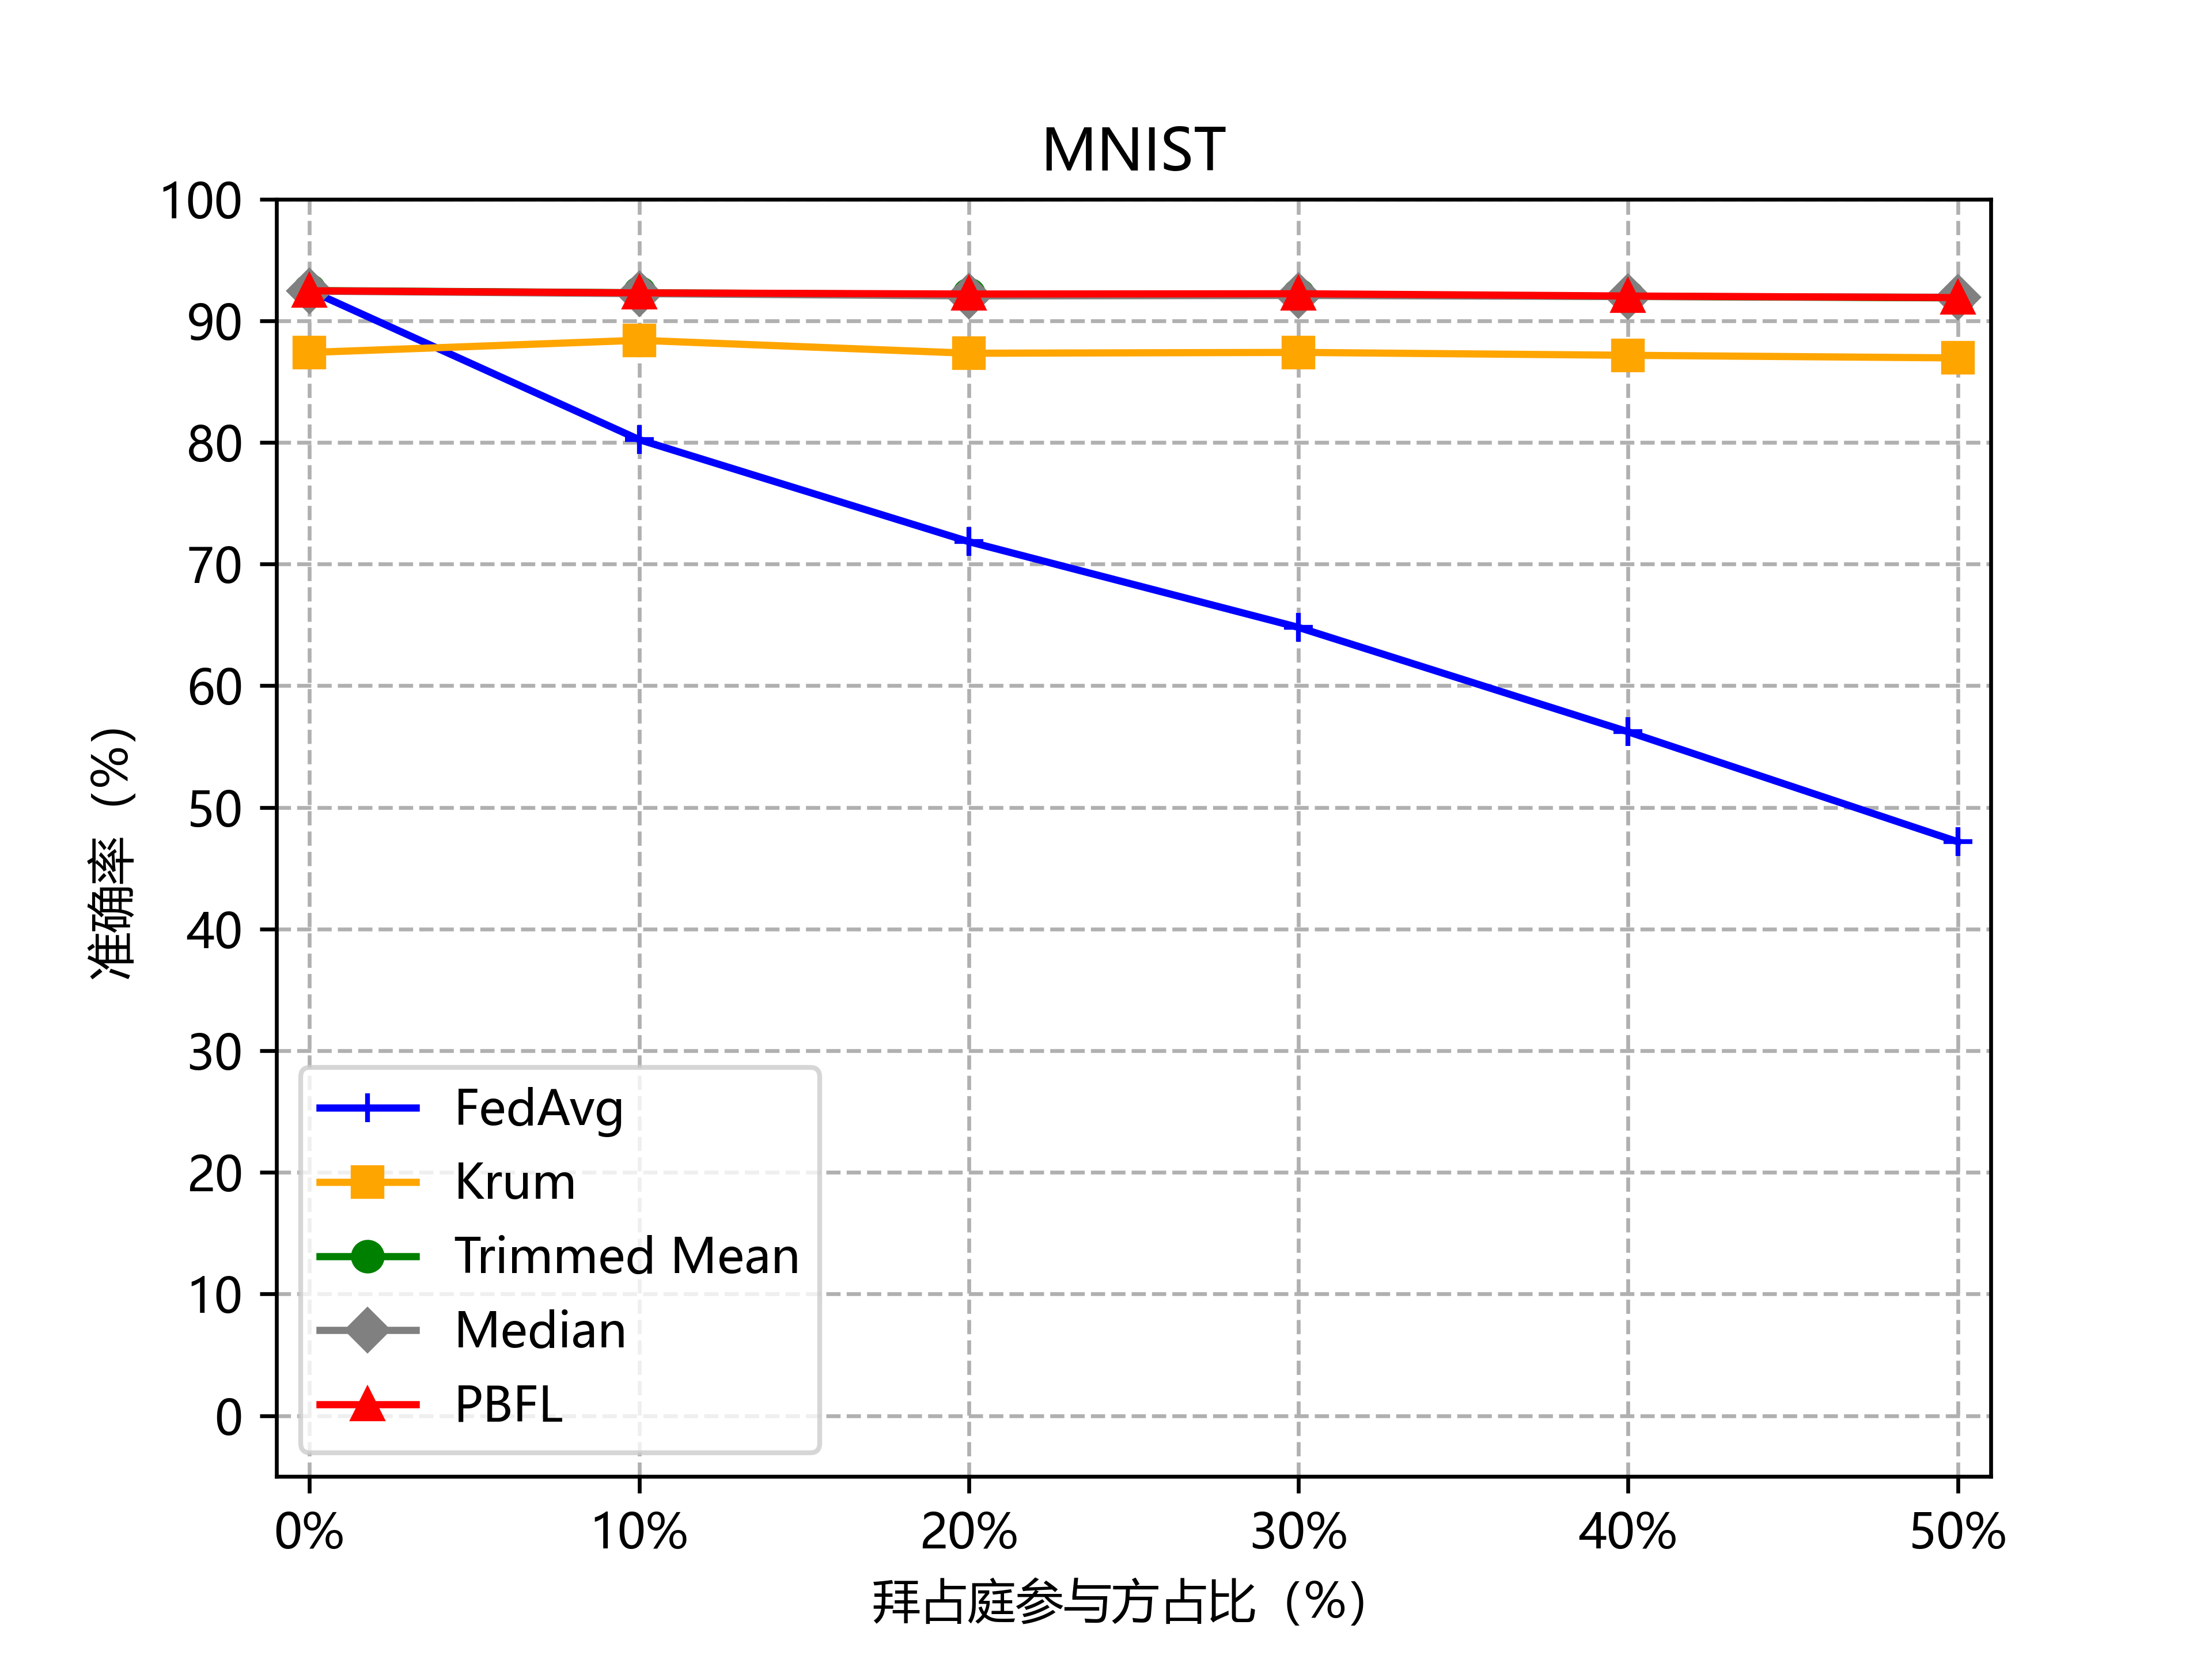
\includegraphics[width=\linewidth]{img/mnist-GA-win-1.png}
			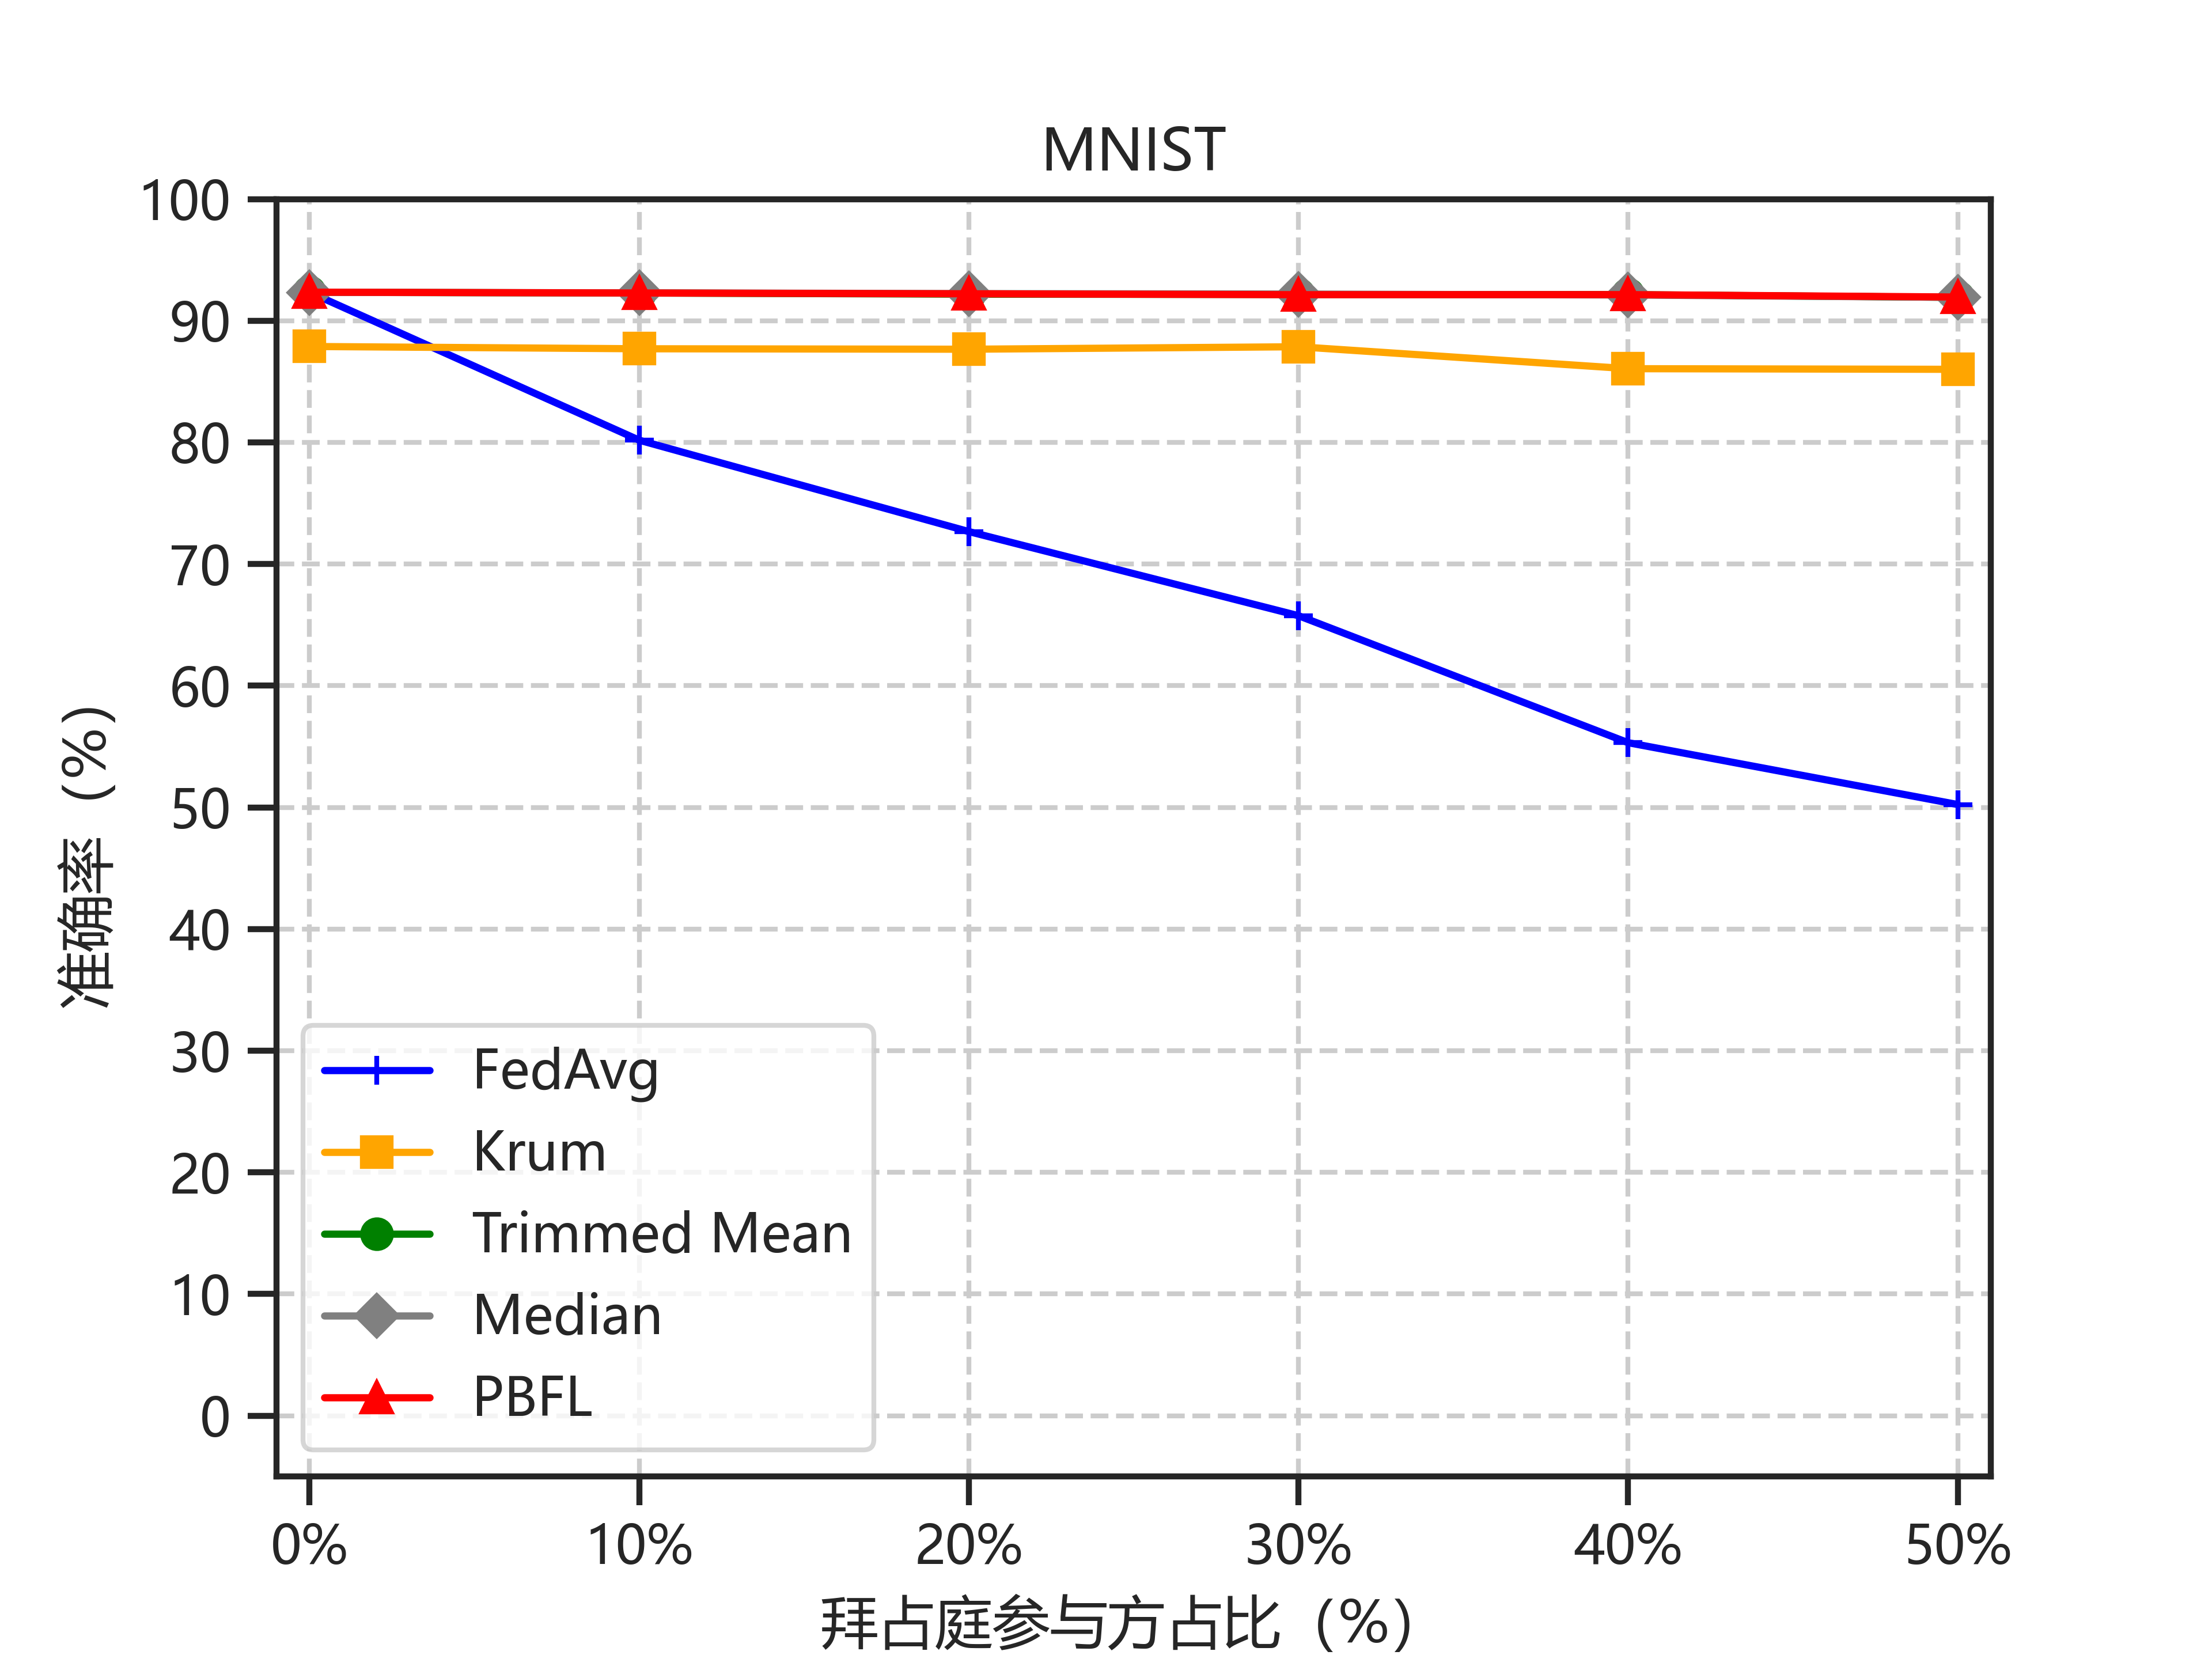
\includegraphics[width=\linewidth]{img/repeat/mnist-GA200-win-repeat.png}
		\end{minipage}
	}
	\subfloat[GA攻击(CIFAR-10)]{
	\begin{minipage}[b]{0.48\textwidth}
		\centering
		\label{fig2:b}
%		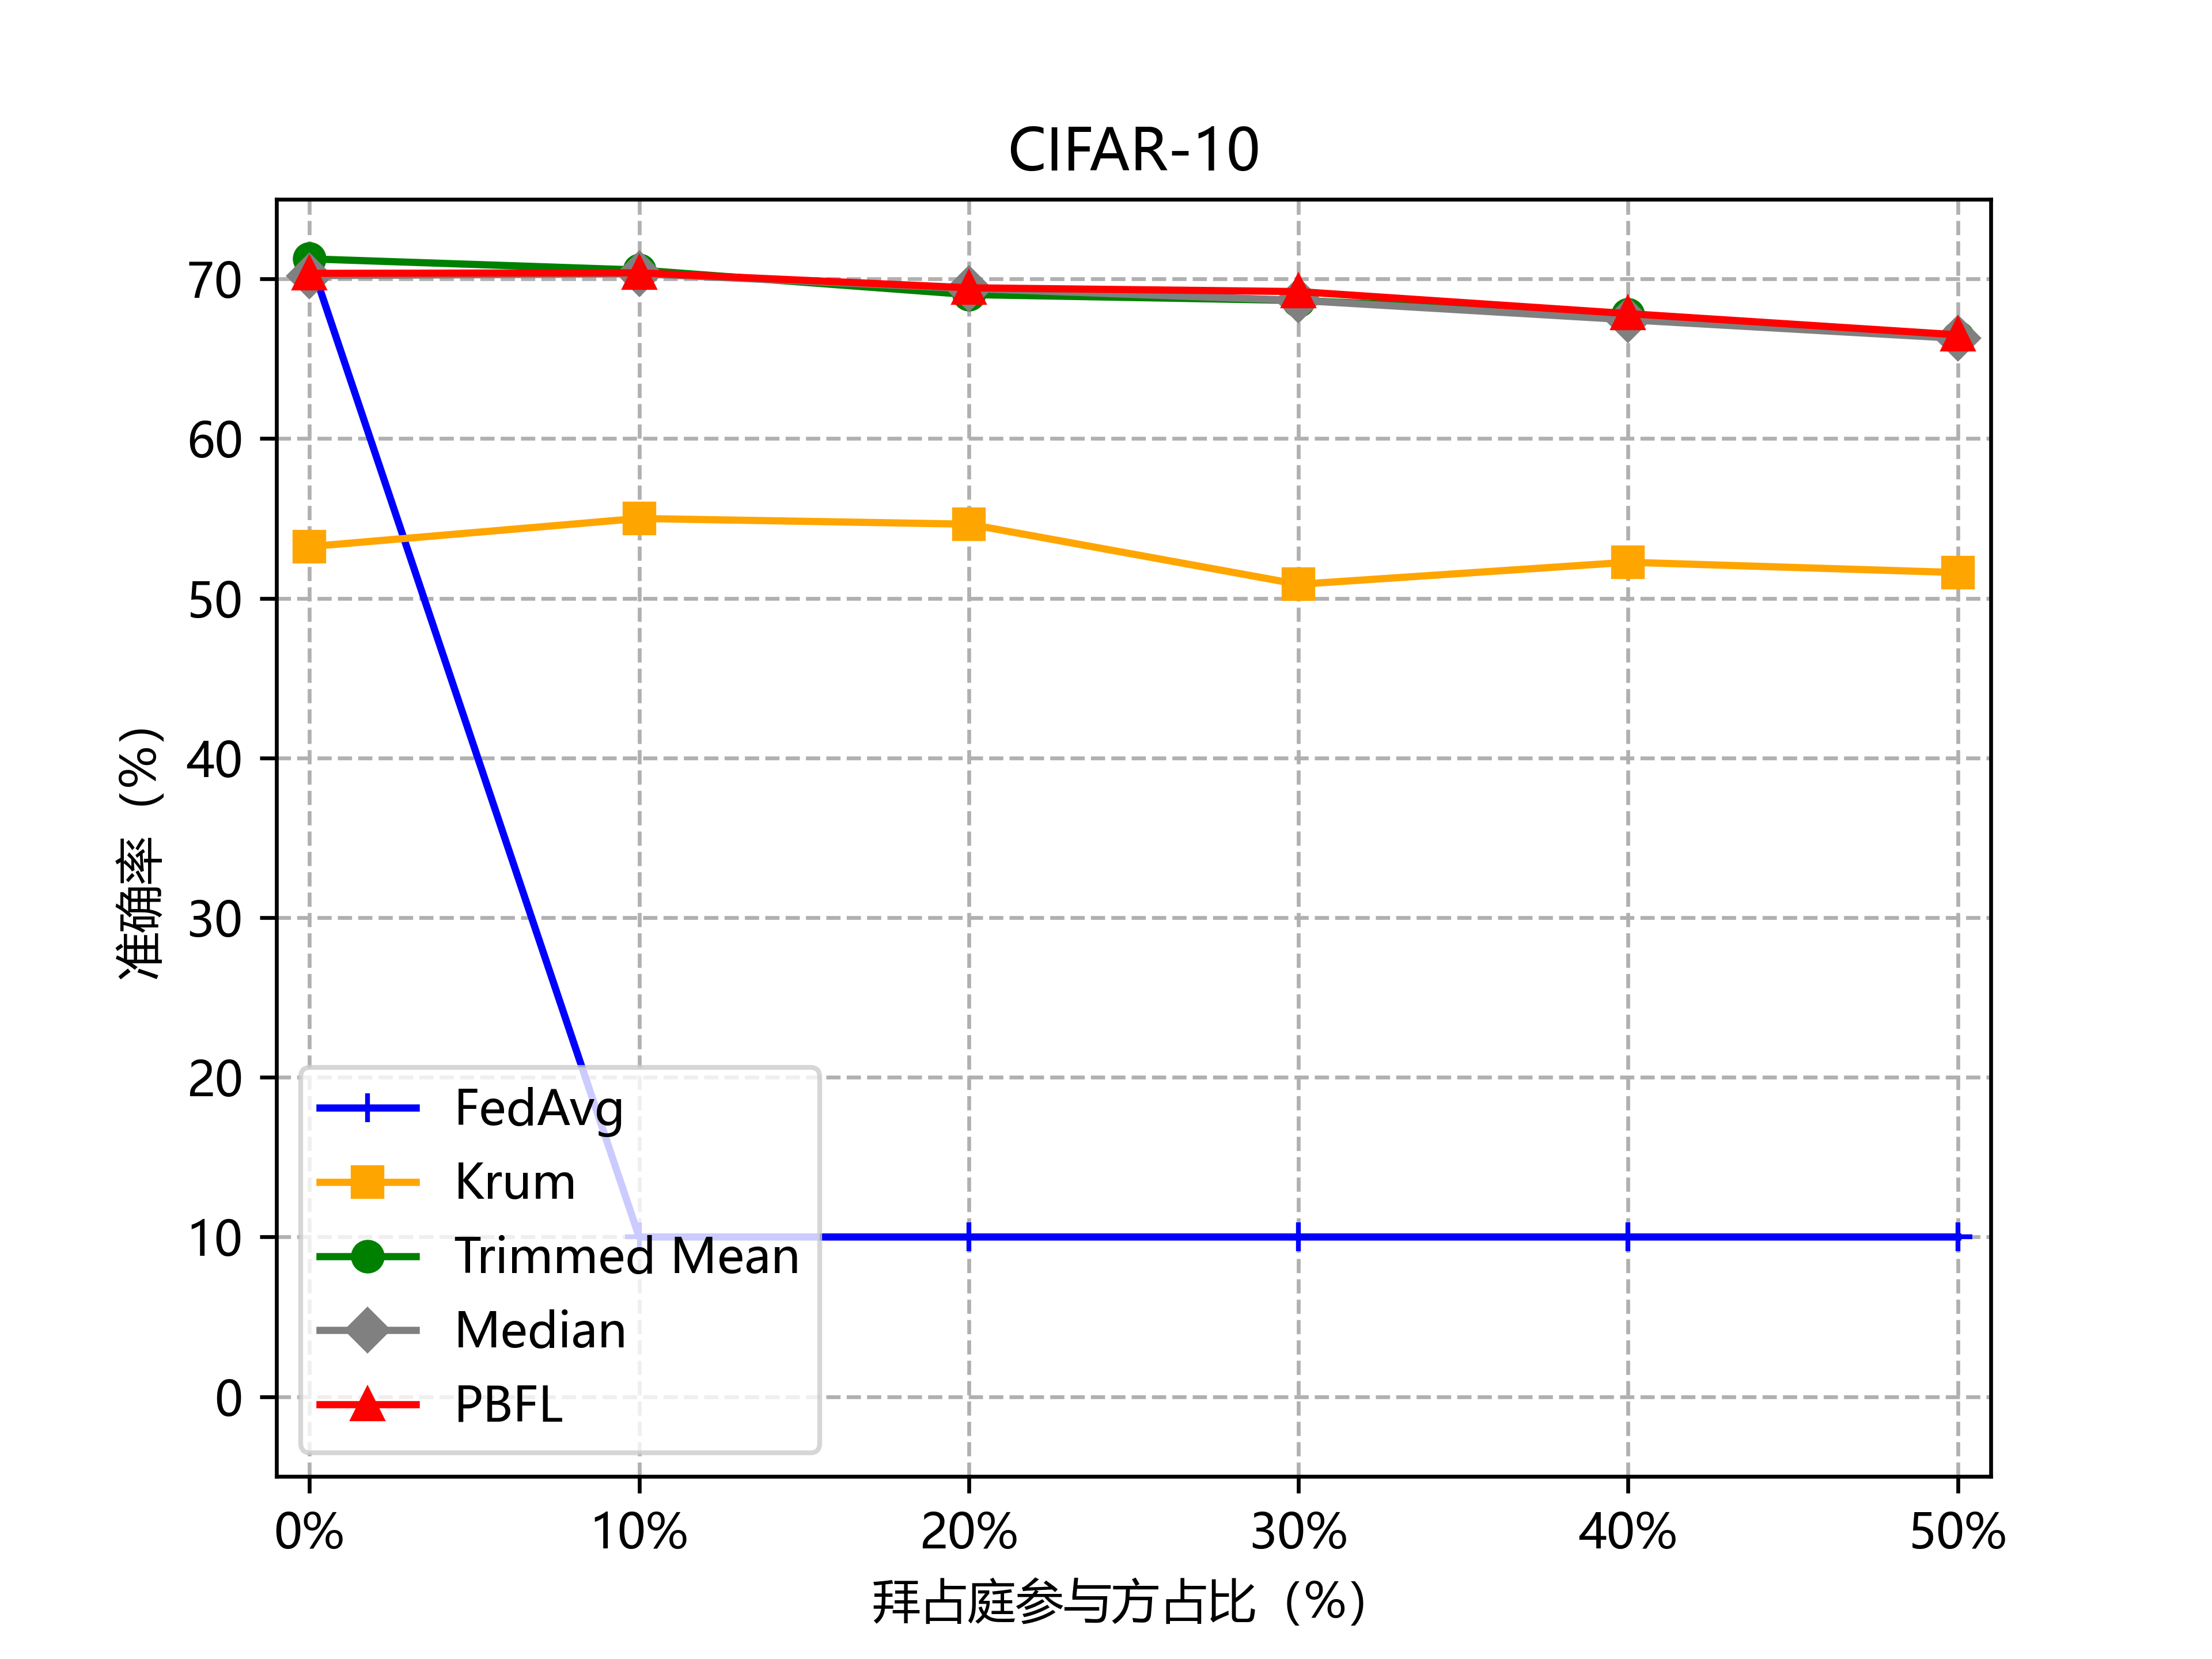
\includegraphics[width=\linewidth]{img/cifar-GA-win-1.png}
		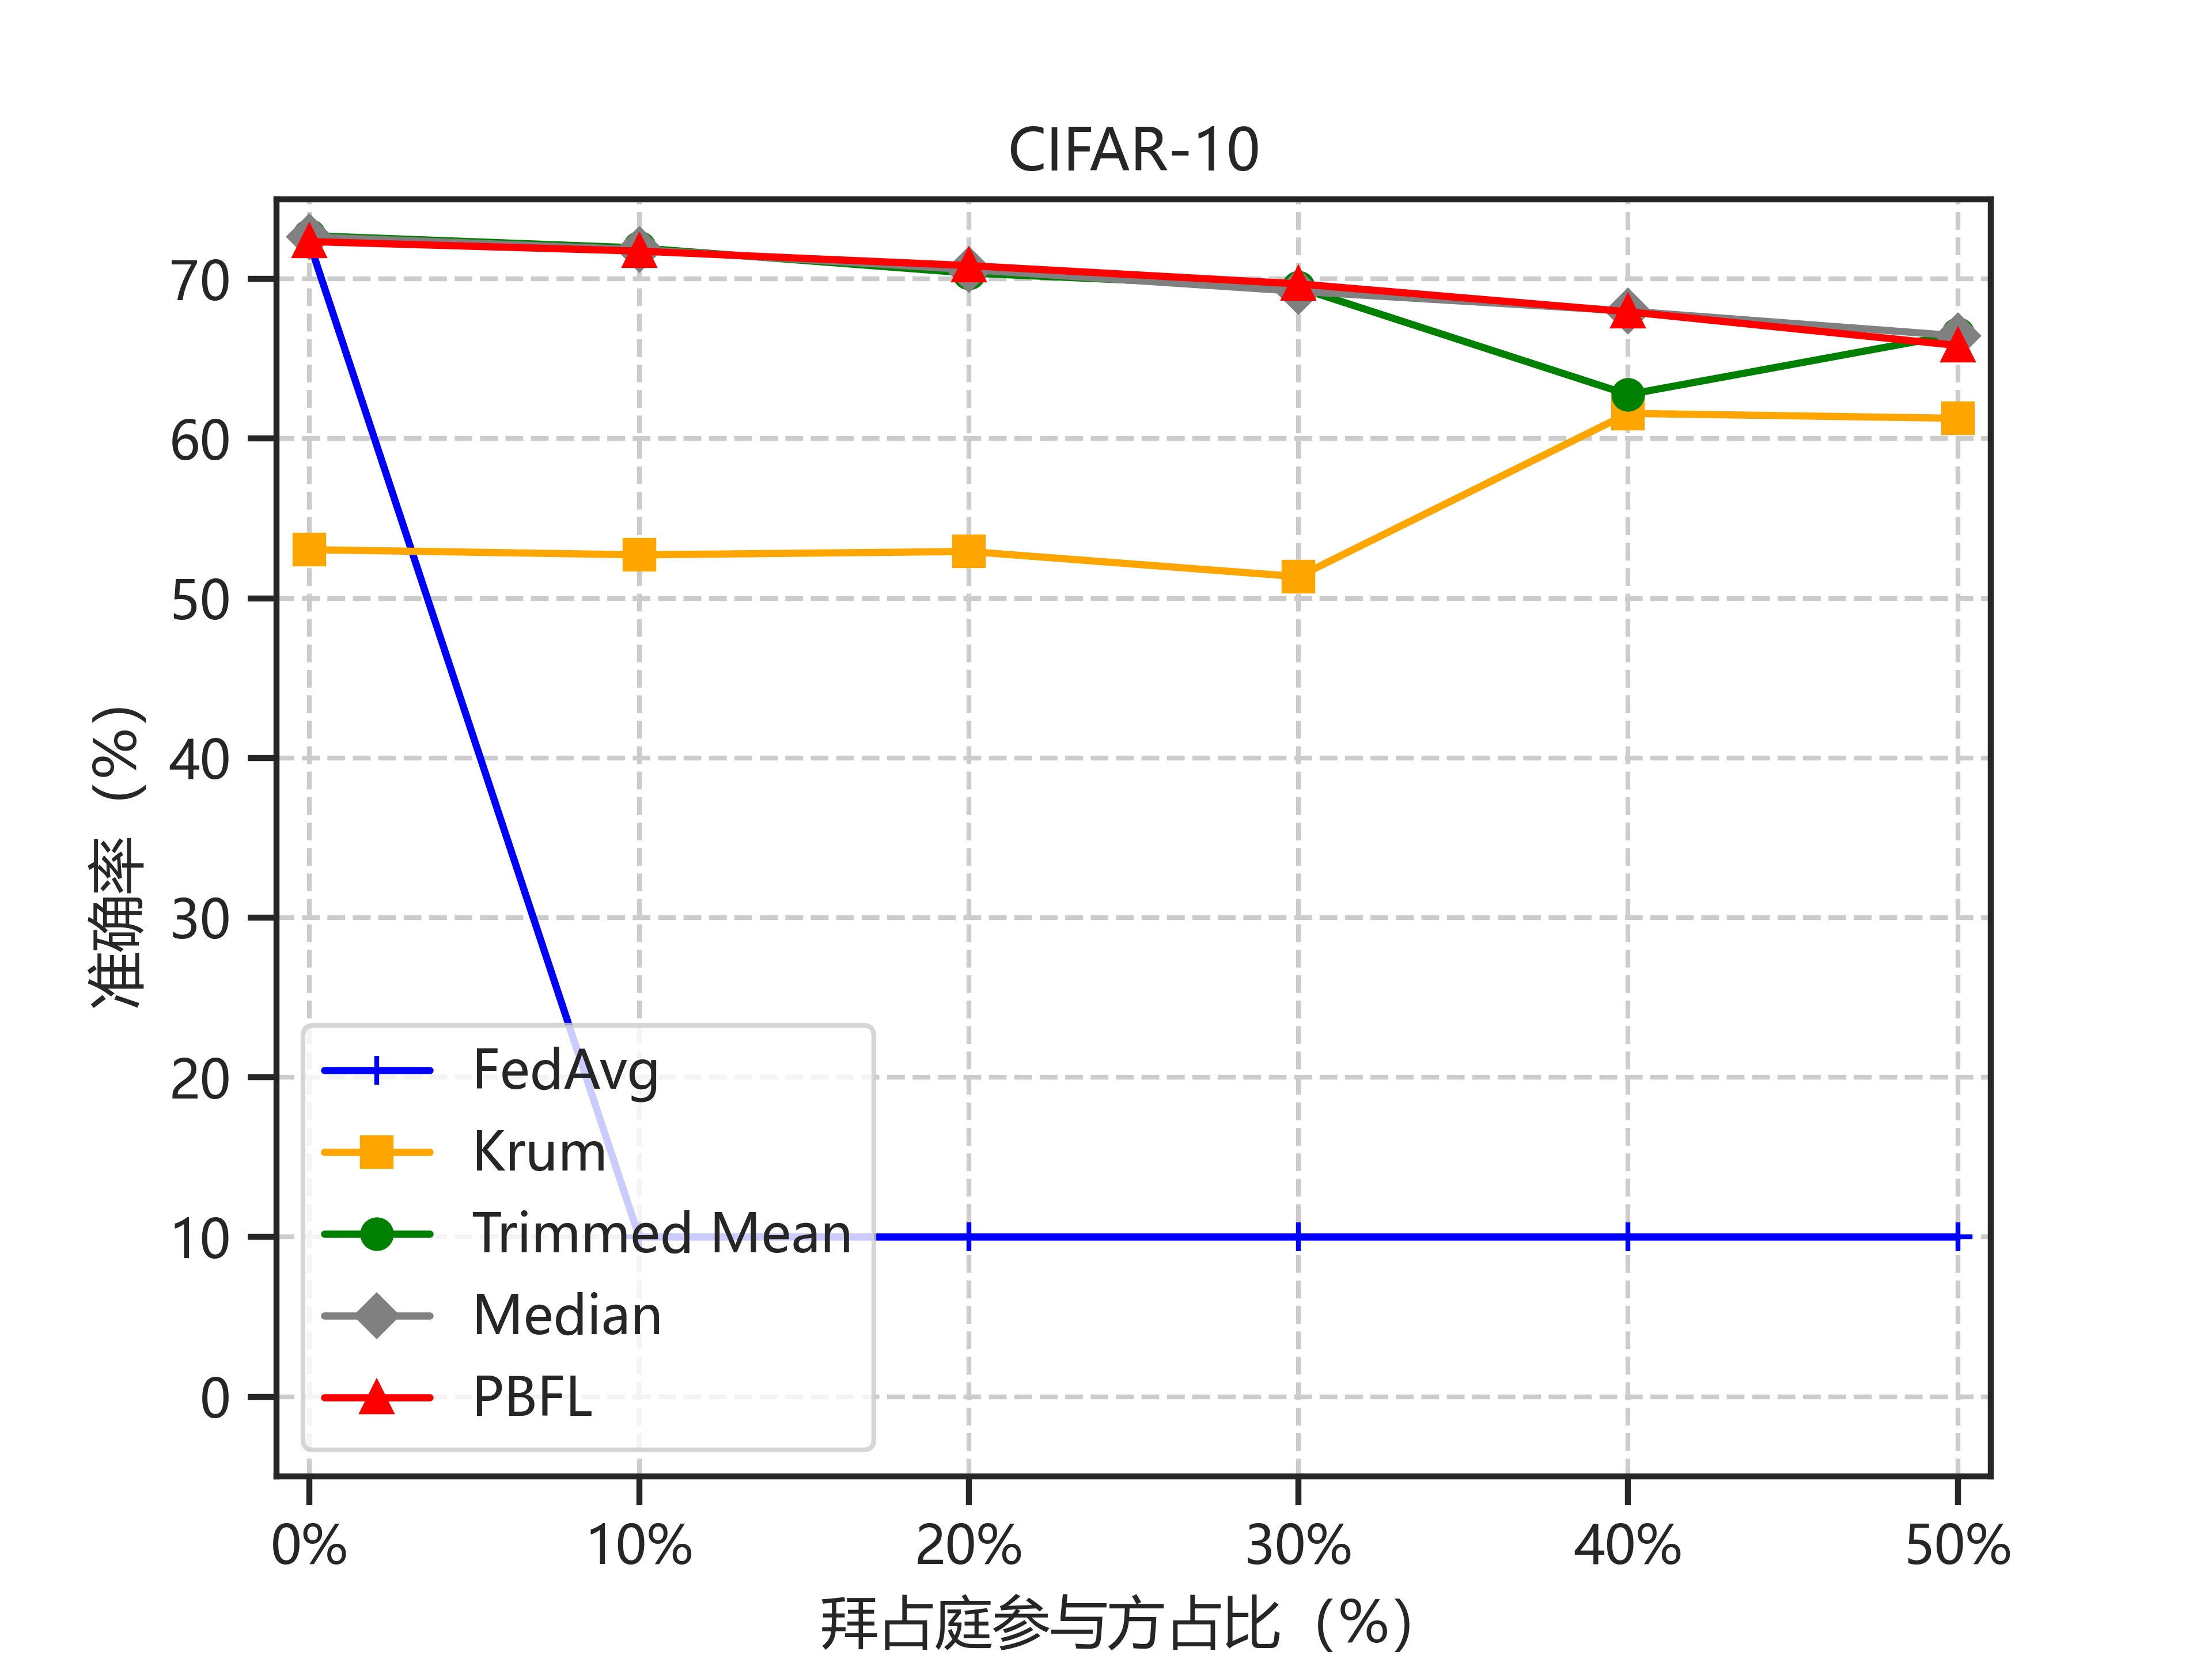
\includegraphics[width=\linewidth]{img/repeat/cifar-GA200-win-repeat.png}
	\end{minipage}
	}


%	\hspace{-1.0in}
%	\vspace{-0.12in}
	\subfloat[LFA攻击(MNIST)]{
	\begin{minipage}[b]{0.48\textwidth}
		\centering
		\label{fig2:c}
%		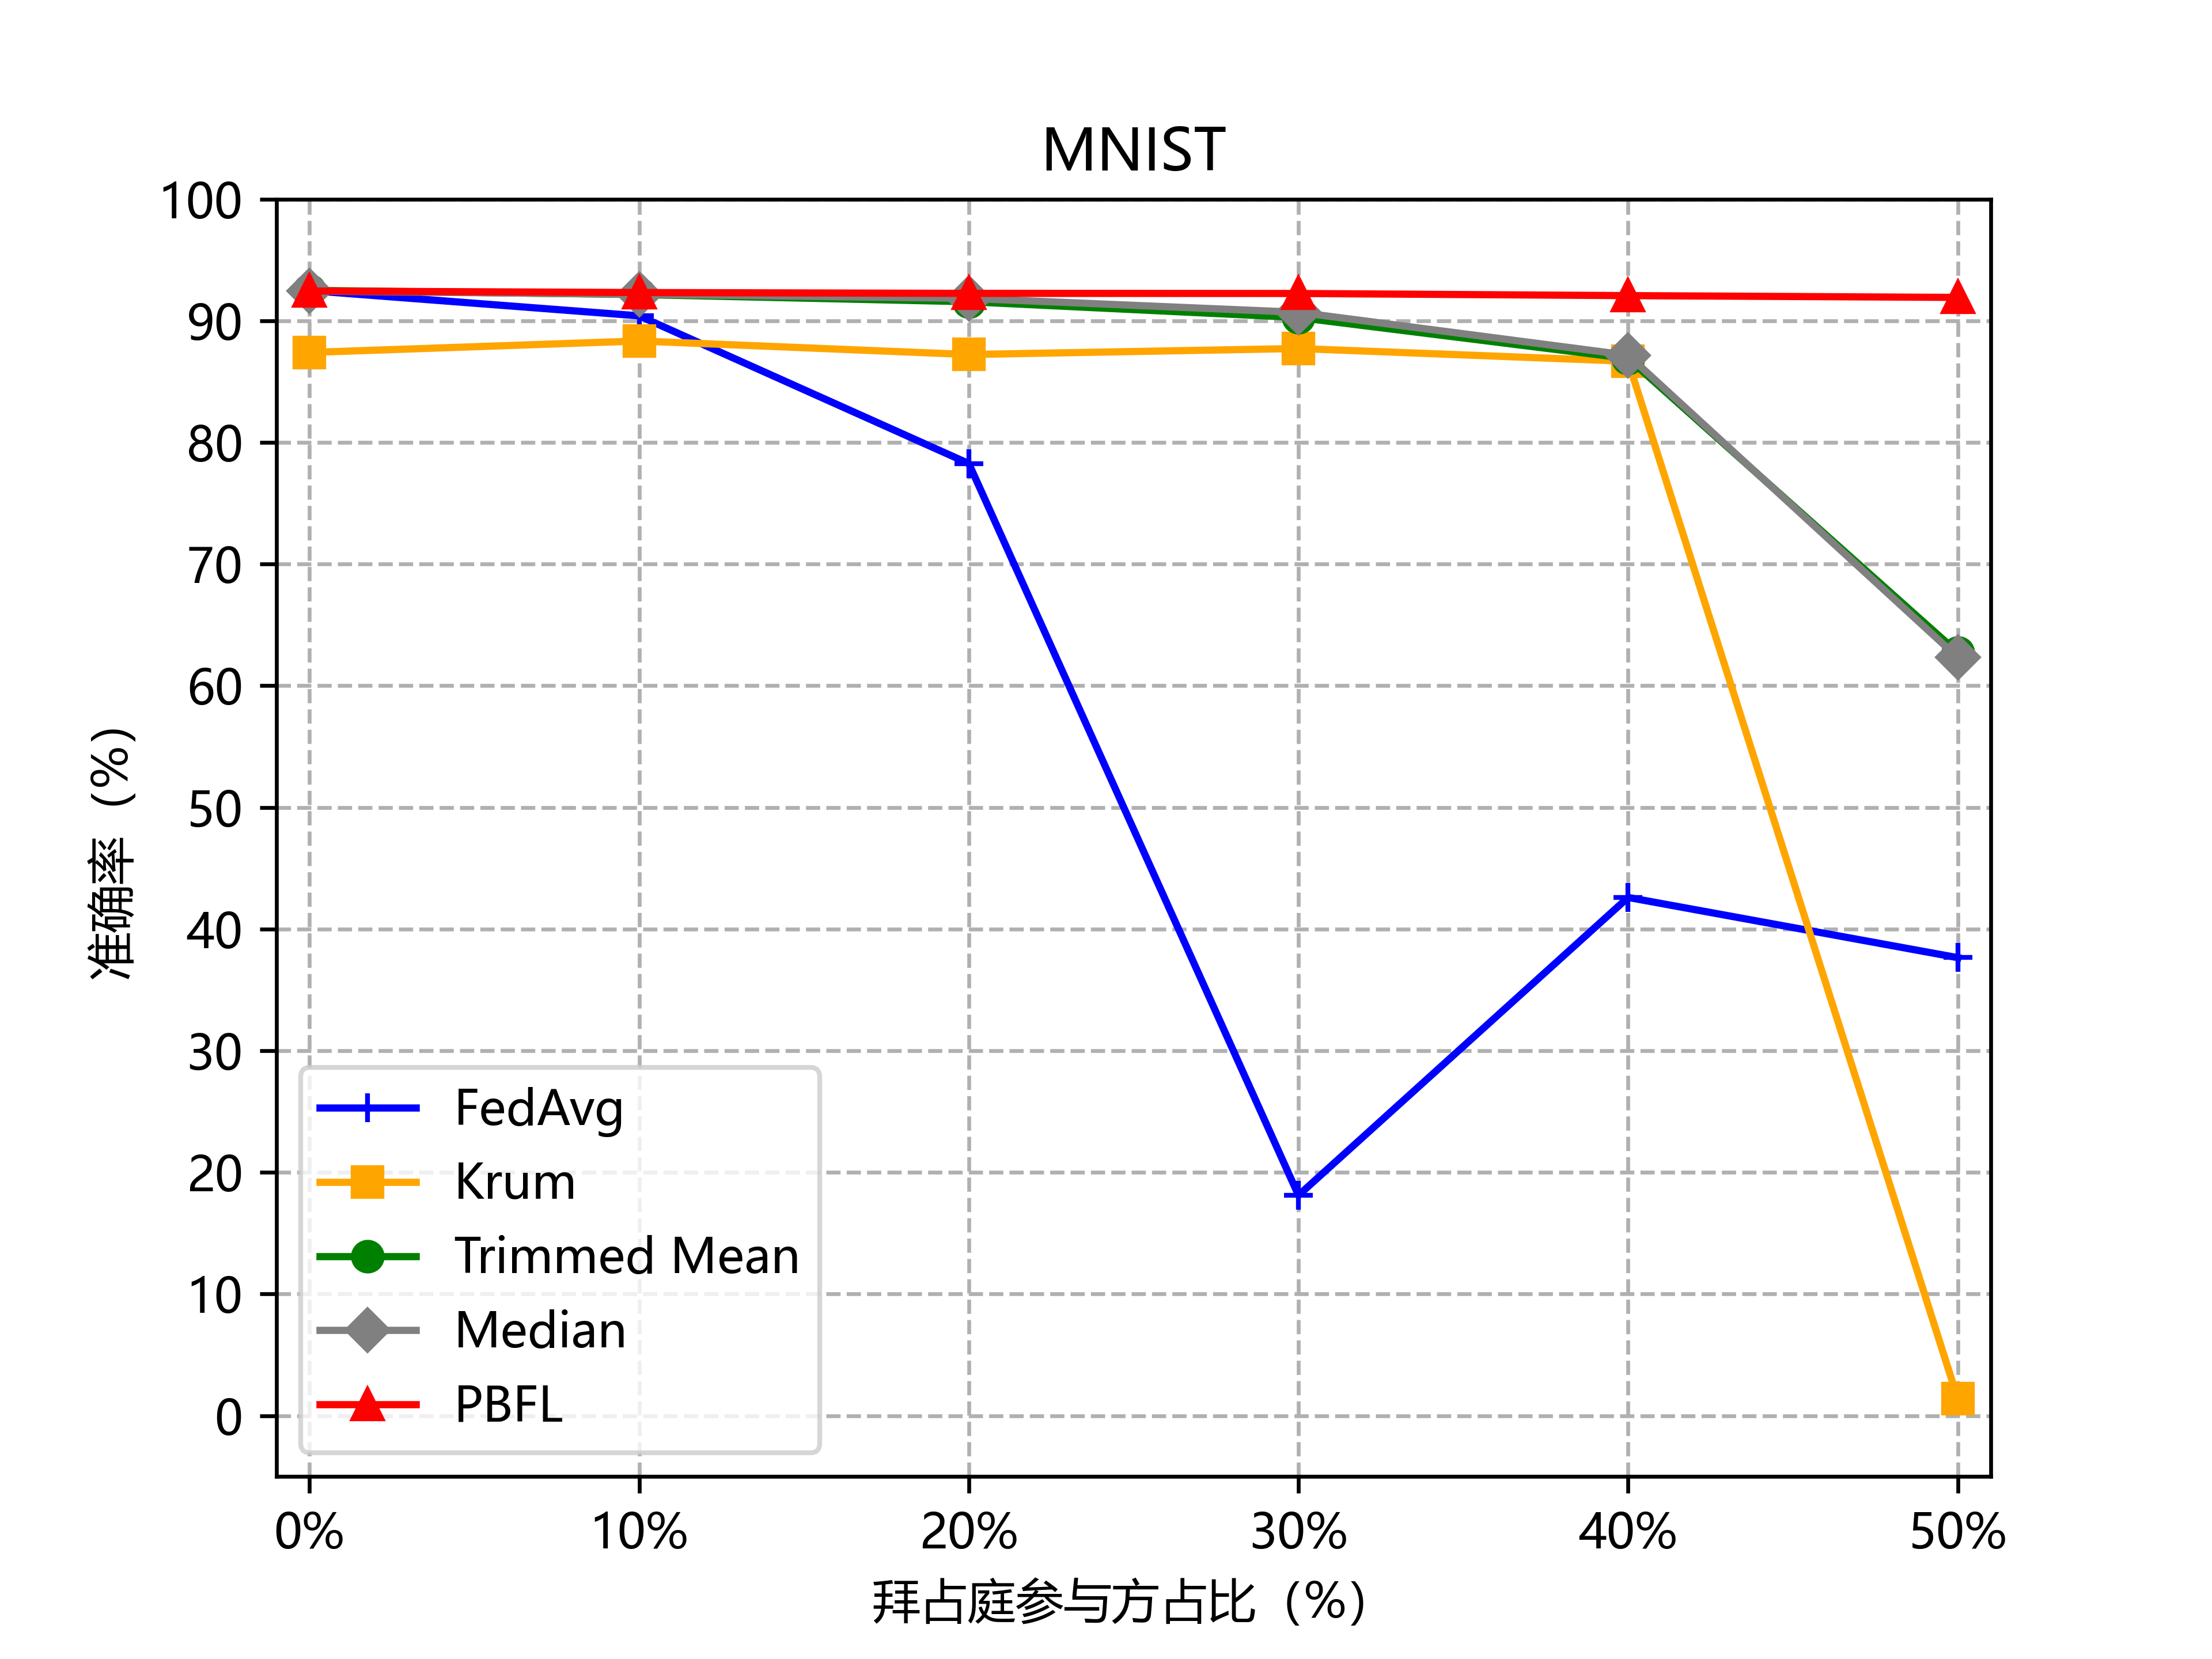
\includegraphics[width=\linewidth]{img/mnist-LF-win-1.png}
		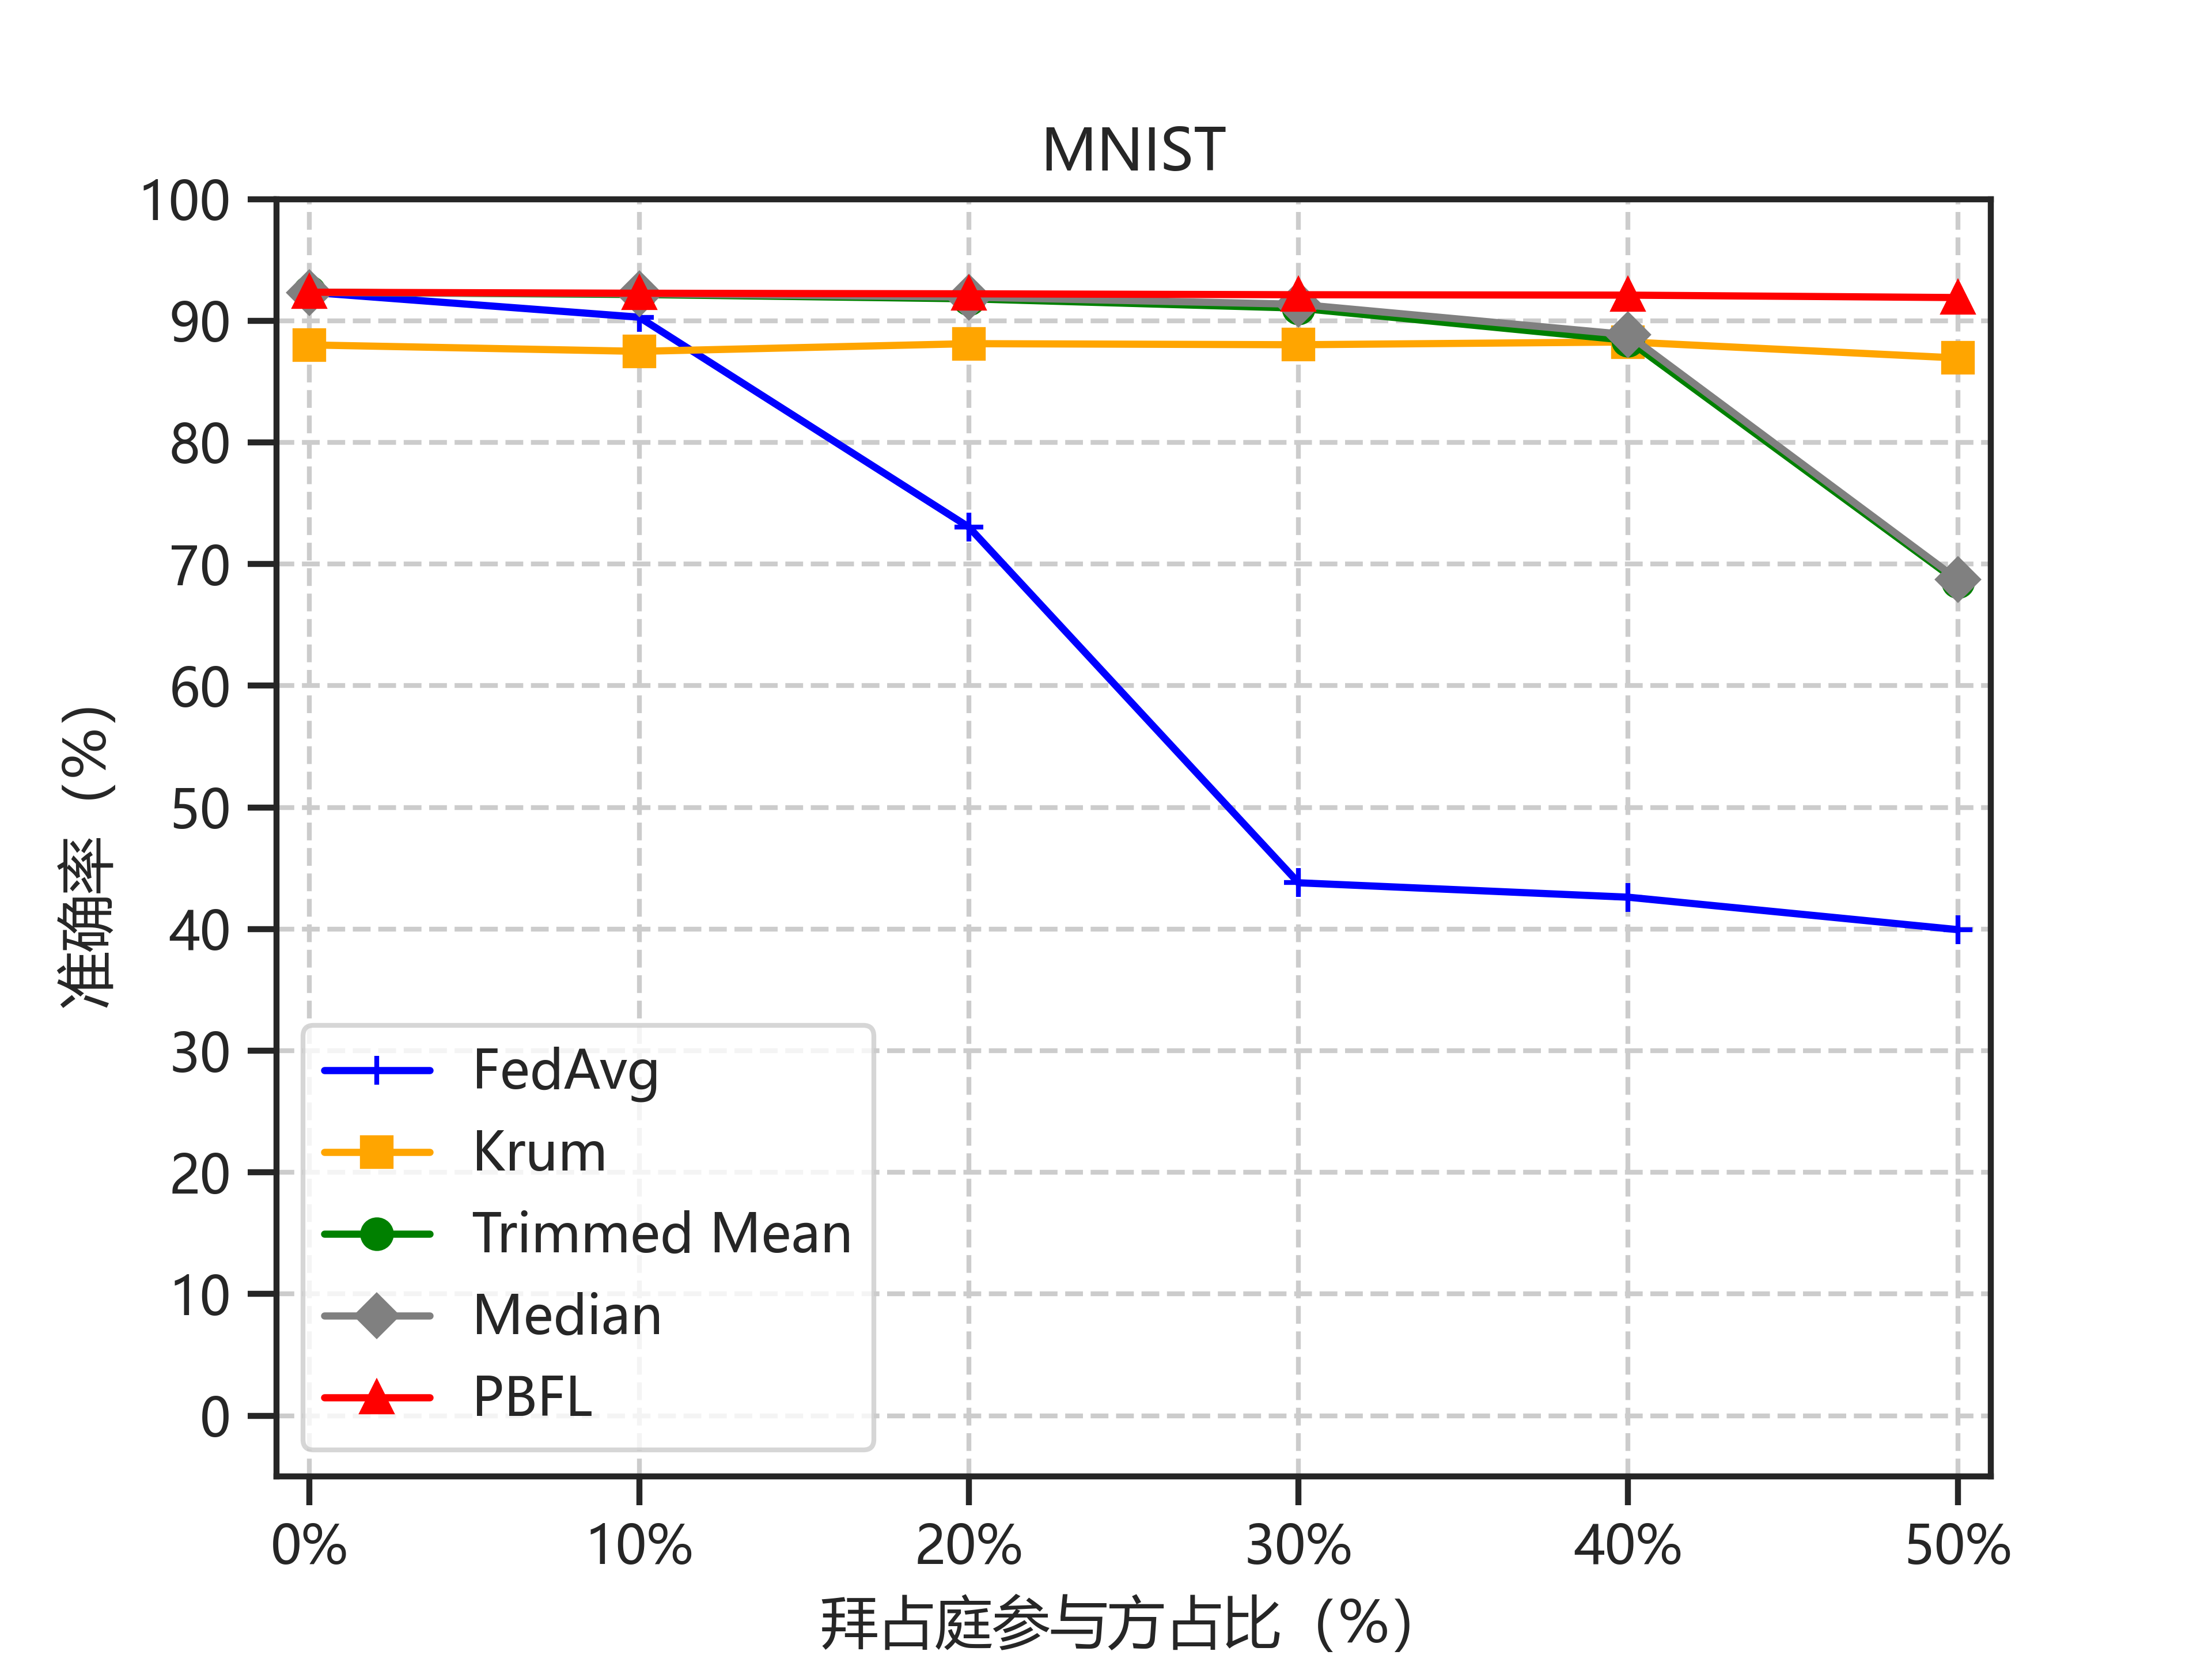
\includegraphics[width=\linewidth]{img/repeat/mnist-LF-win-repeat.png}
	\end{minipage}
	}
%	\hspace{-1.0in}
	\subfloat[LFA攻击(CIFAR-10)]{
		\begin{minipage}[b]{0.48\textwidth}
			\centering
			\label{fig2:d}
%			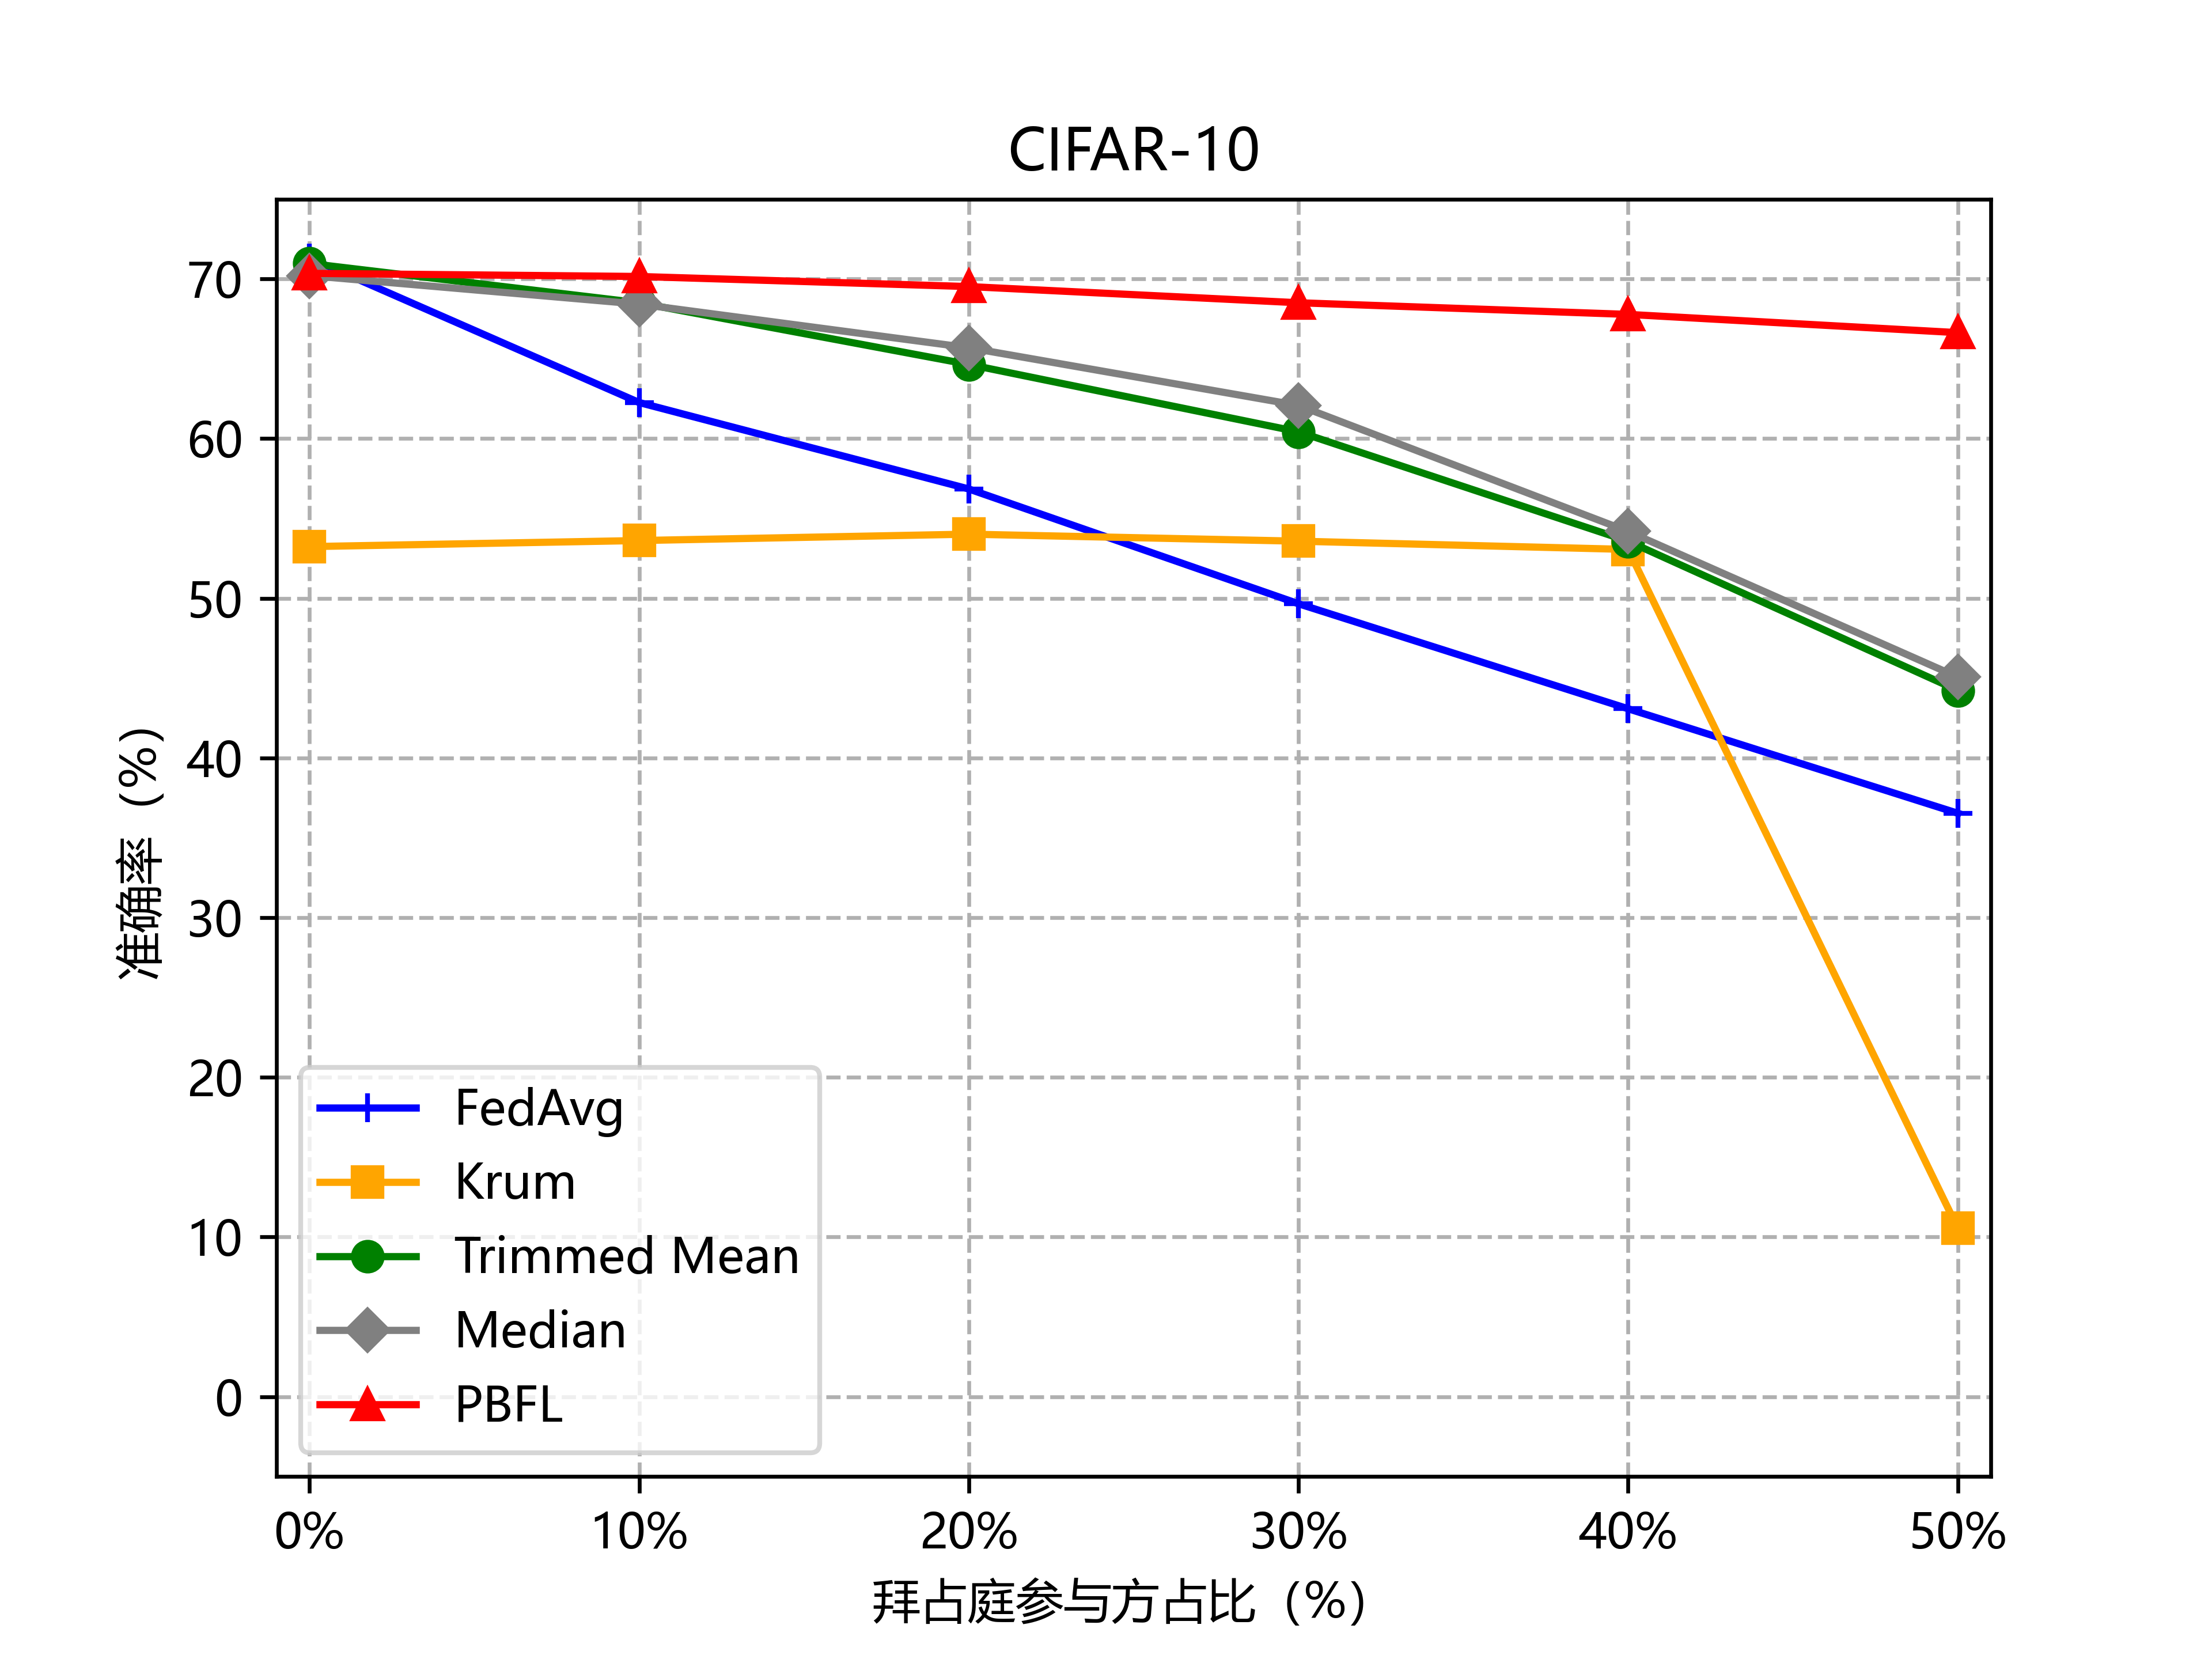
\includegraphics[width=\linewidth]{img/cifar-LF-win-1.png}
			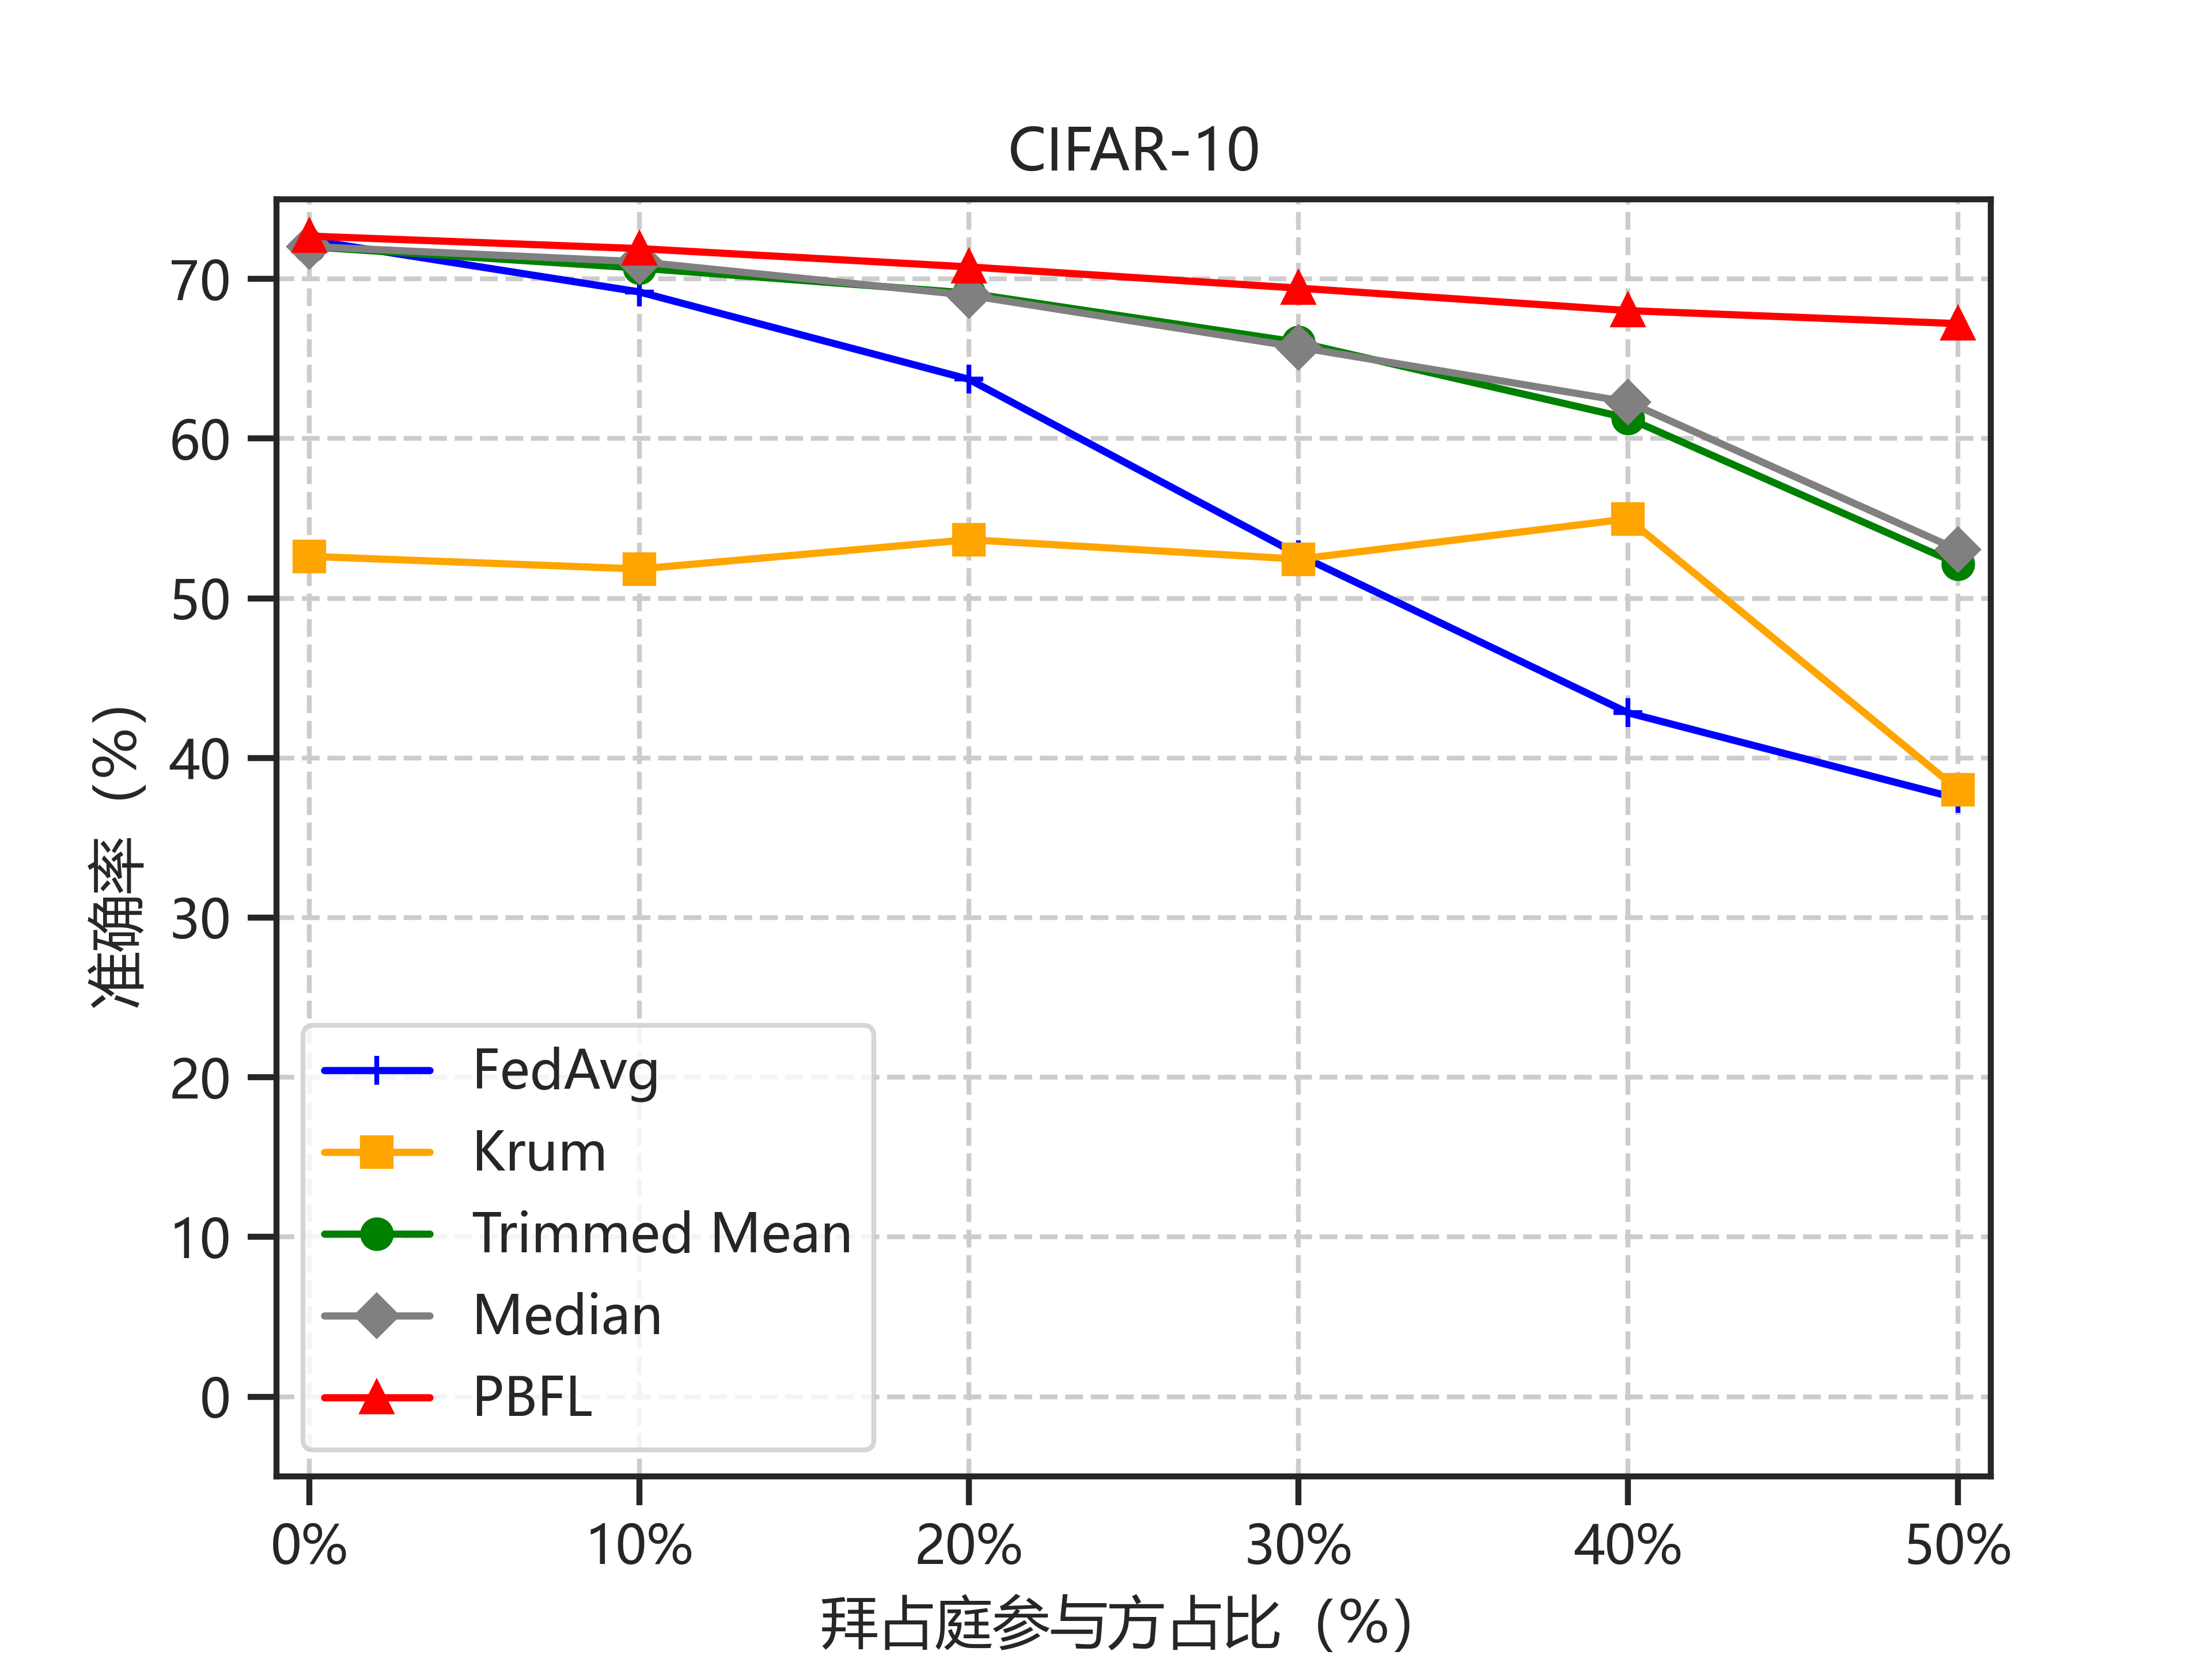
\includegraphics[width=\linewidth]{img/repeat/cifar-LF-win-repeat.png}
		\end{minipage}
	}
	\caption{不同拜占庭参与方占比对准确率的影响}
	\label{fig2}
\end{figure}

\textbf{训练轮次对准确率的影响:}随着训练轮次的增加,全局模型可以更好的捕捉有效数据的特征,进而获取较高的全局模型准确率。
本小节不考虑由模型过小或过大造成的欠拟合或者过拟合,主要比较不同方案之间的准确率差异。
在图\ref{f3}中,对比了三种防御方案在不同训练轮次的全局模型准确率表现,其中选择的三种方案是上文中表现相对较好的方案,分别是本章方案PBFL、Median和Trimmed Mean。
本文将恶意节点占比固定为$20\%$,即将$51$个用户中的10个设置为拜占庭参与方。
然后在图\ref{f3}中,展示了三种方案在不同攻击下,最后100轮次的准确率变化,可以观察到PBFL整体上在准确率和稳定性上稍优于其它两种方案,其中优势在被LFA攻击时最明显。
值得注意的是,对比的其它方案都是基于参数明文来辨别拜占庭参与方,PBFL实现了密文上的恶意用户过滤,同时还做到了性能优于其它方案。

\begin{figure}[htb]
	\centering
	% \vspace{-0.2in}
	\subfloat[GA攻击(MNIST)]{
		\begin{minipage}[b]{0.48\textwidth}
			\centering
			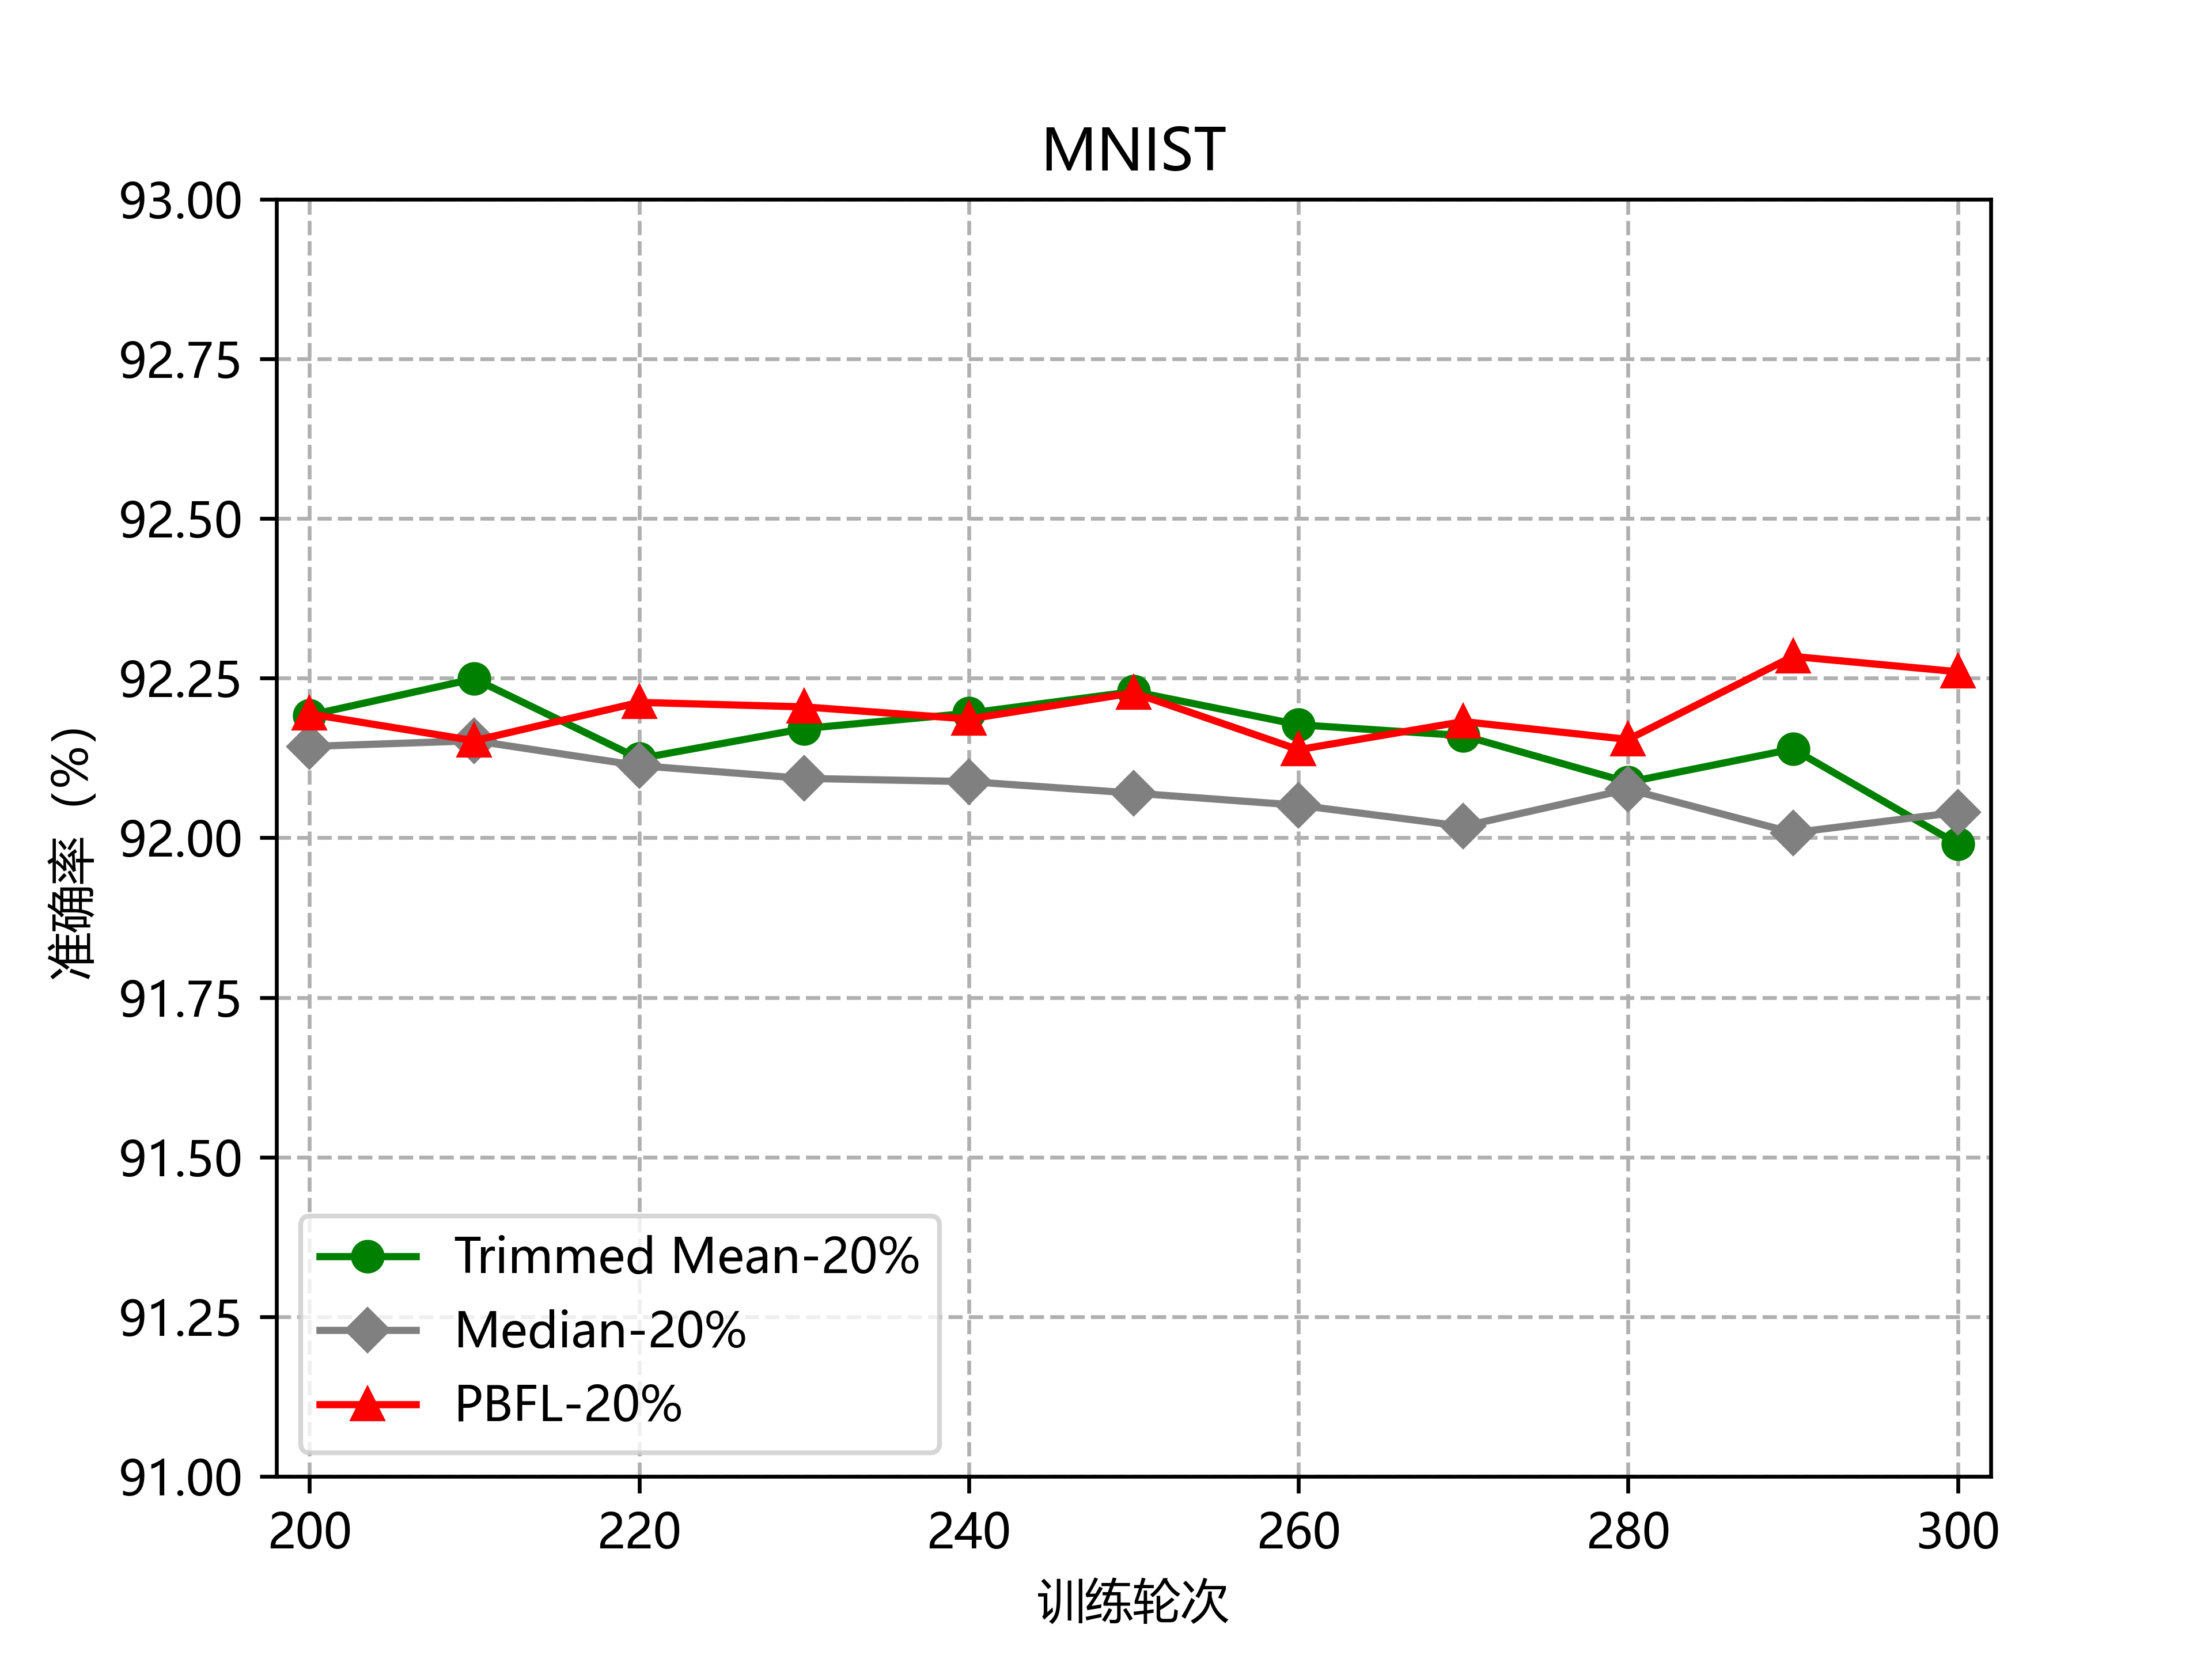
\includegraphics[width=\linewidth]{img/mnist-GA-win-2.png}
		\end{minipage}
	}
%	\hspace{-1.0in}
%	\qquad
	\subfloat[GA攻击(CIFAR-10)]{
	\begin{minipage}[b]{0.48\textwidth}
		\centering
		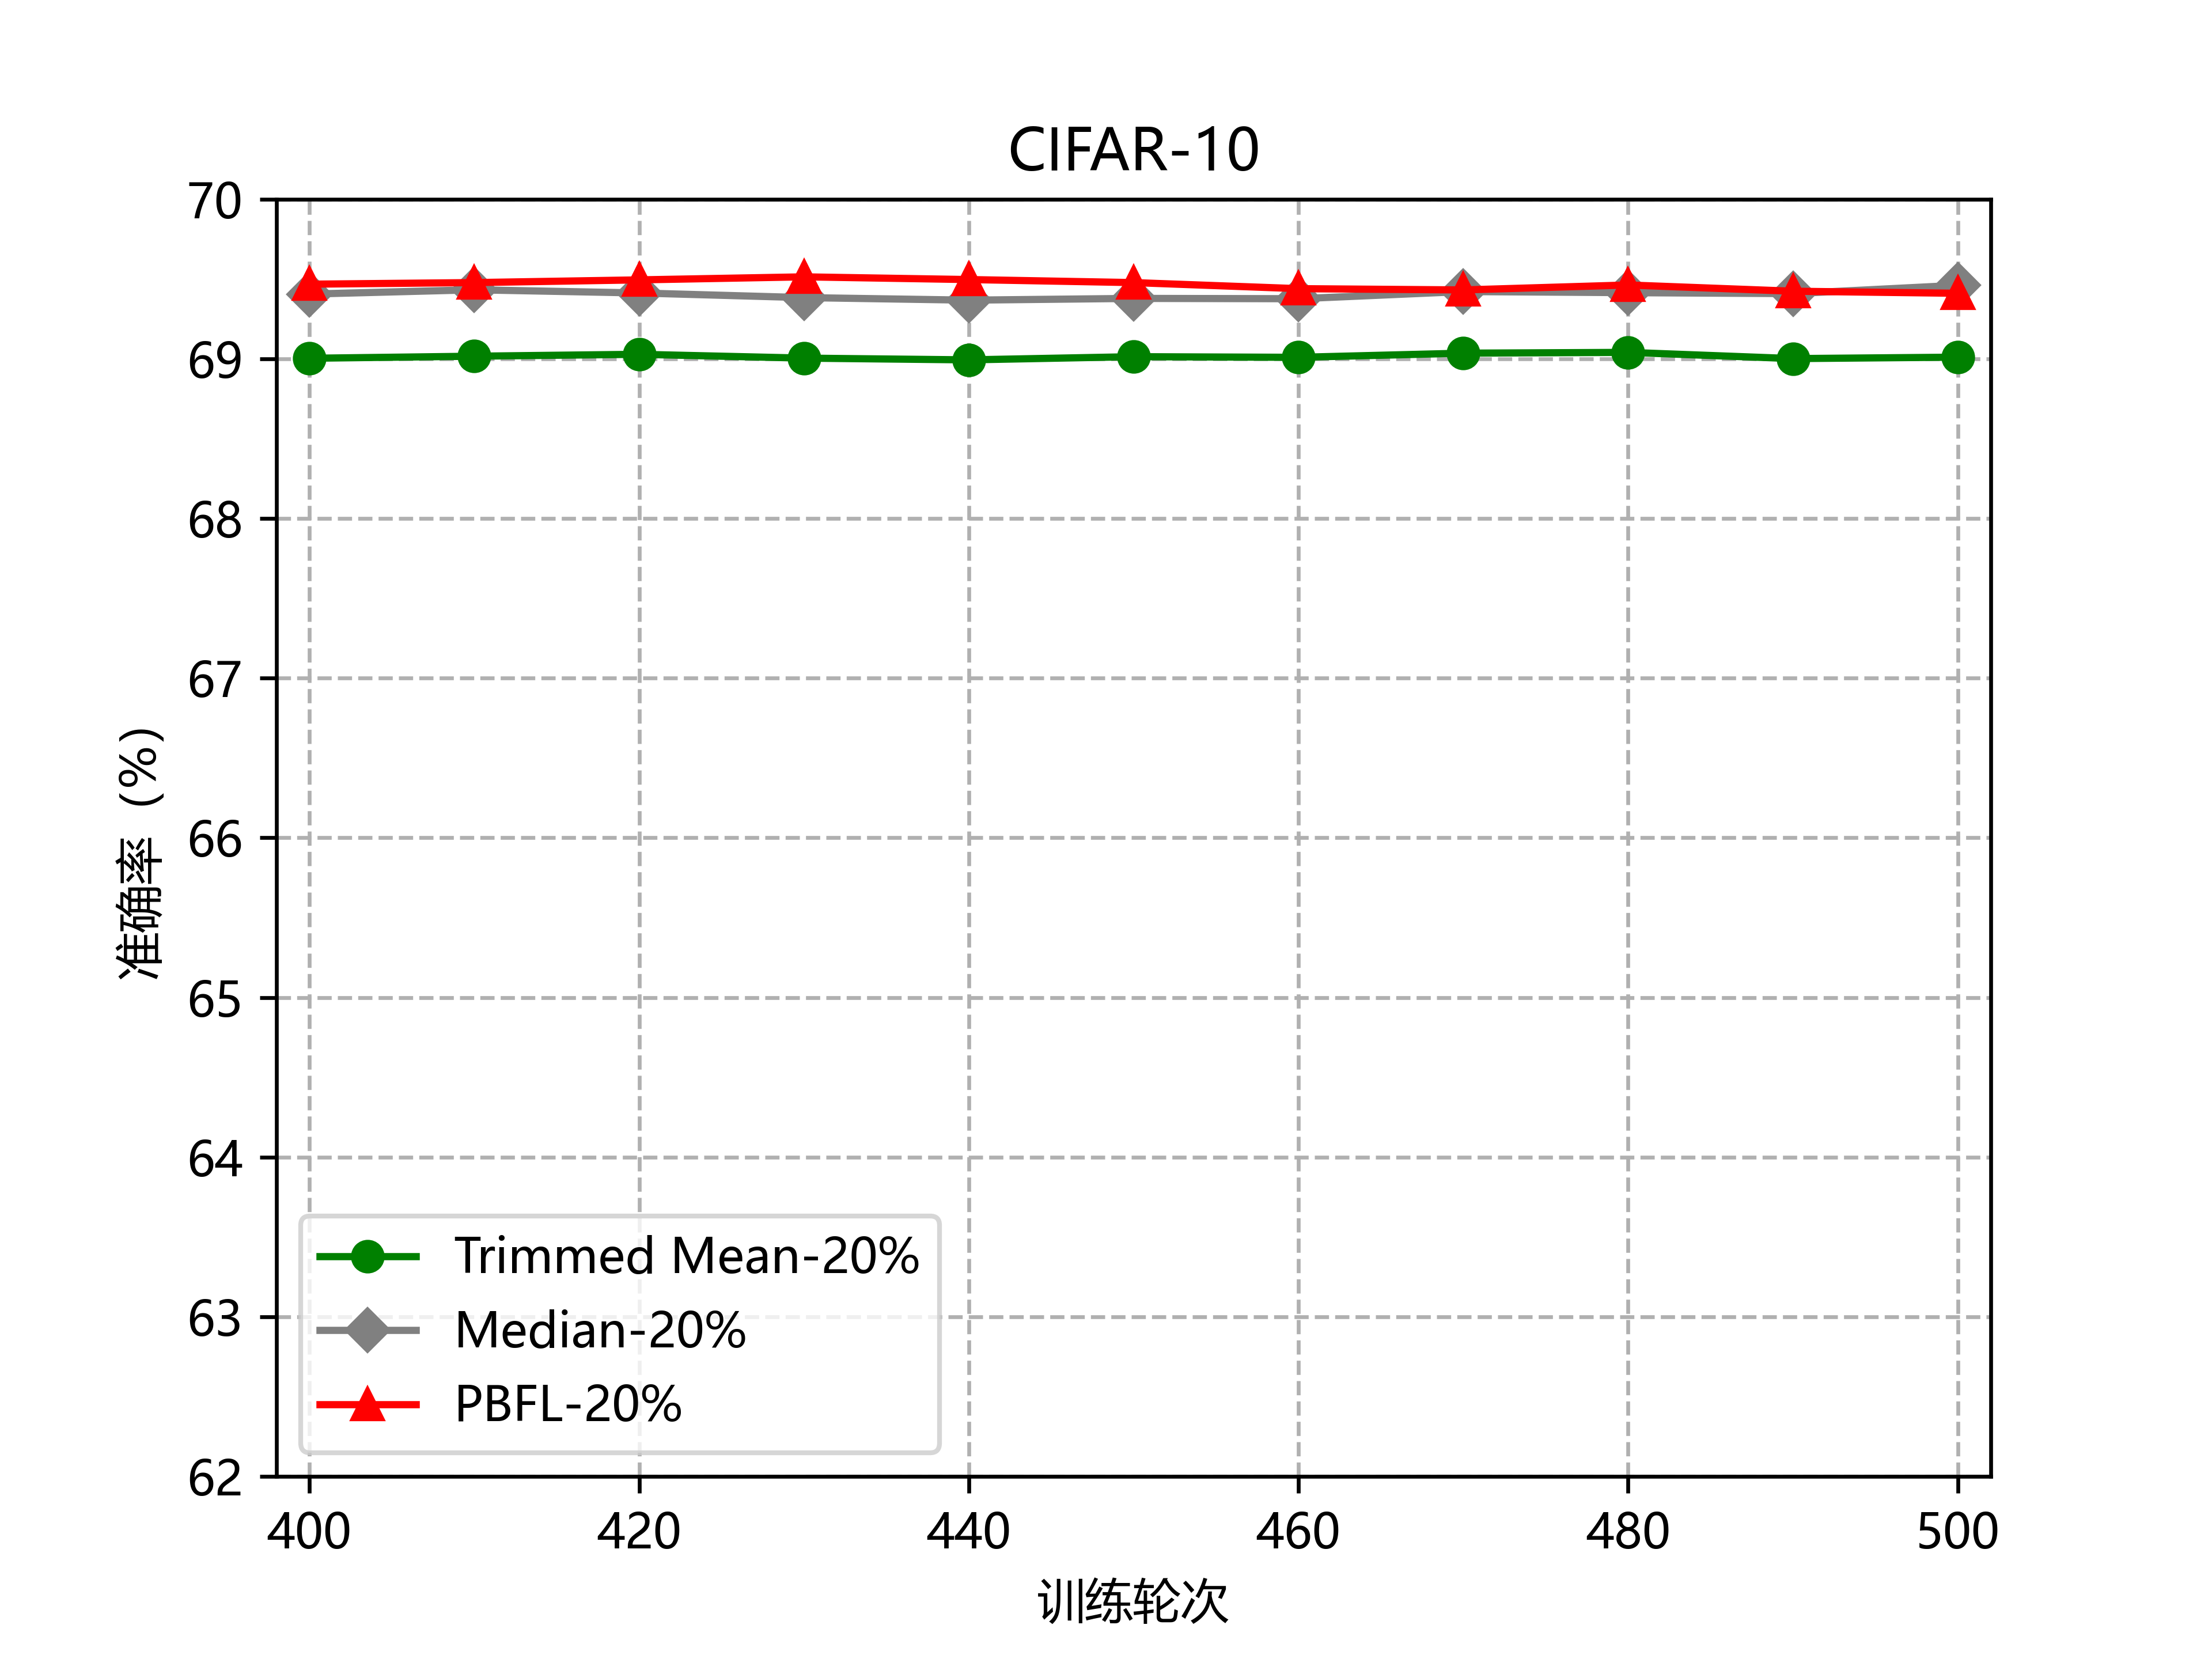
\includegraphics[width=\linewidth]{img/cifar-GA-win-2.png}
	\end{minipage}
}

	
%	\vspace{-0.12in}
	\subfloat[LFA攻击(MNIST)]{
		\begin{minipage}[b]{0.48\textwidth}
			\centering
			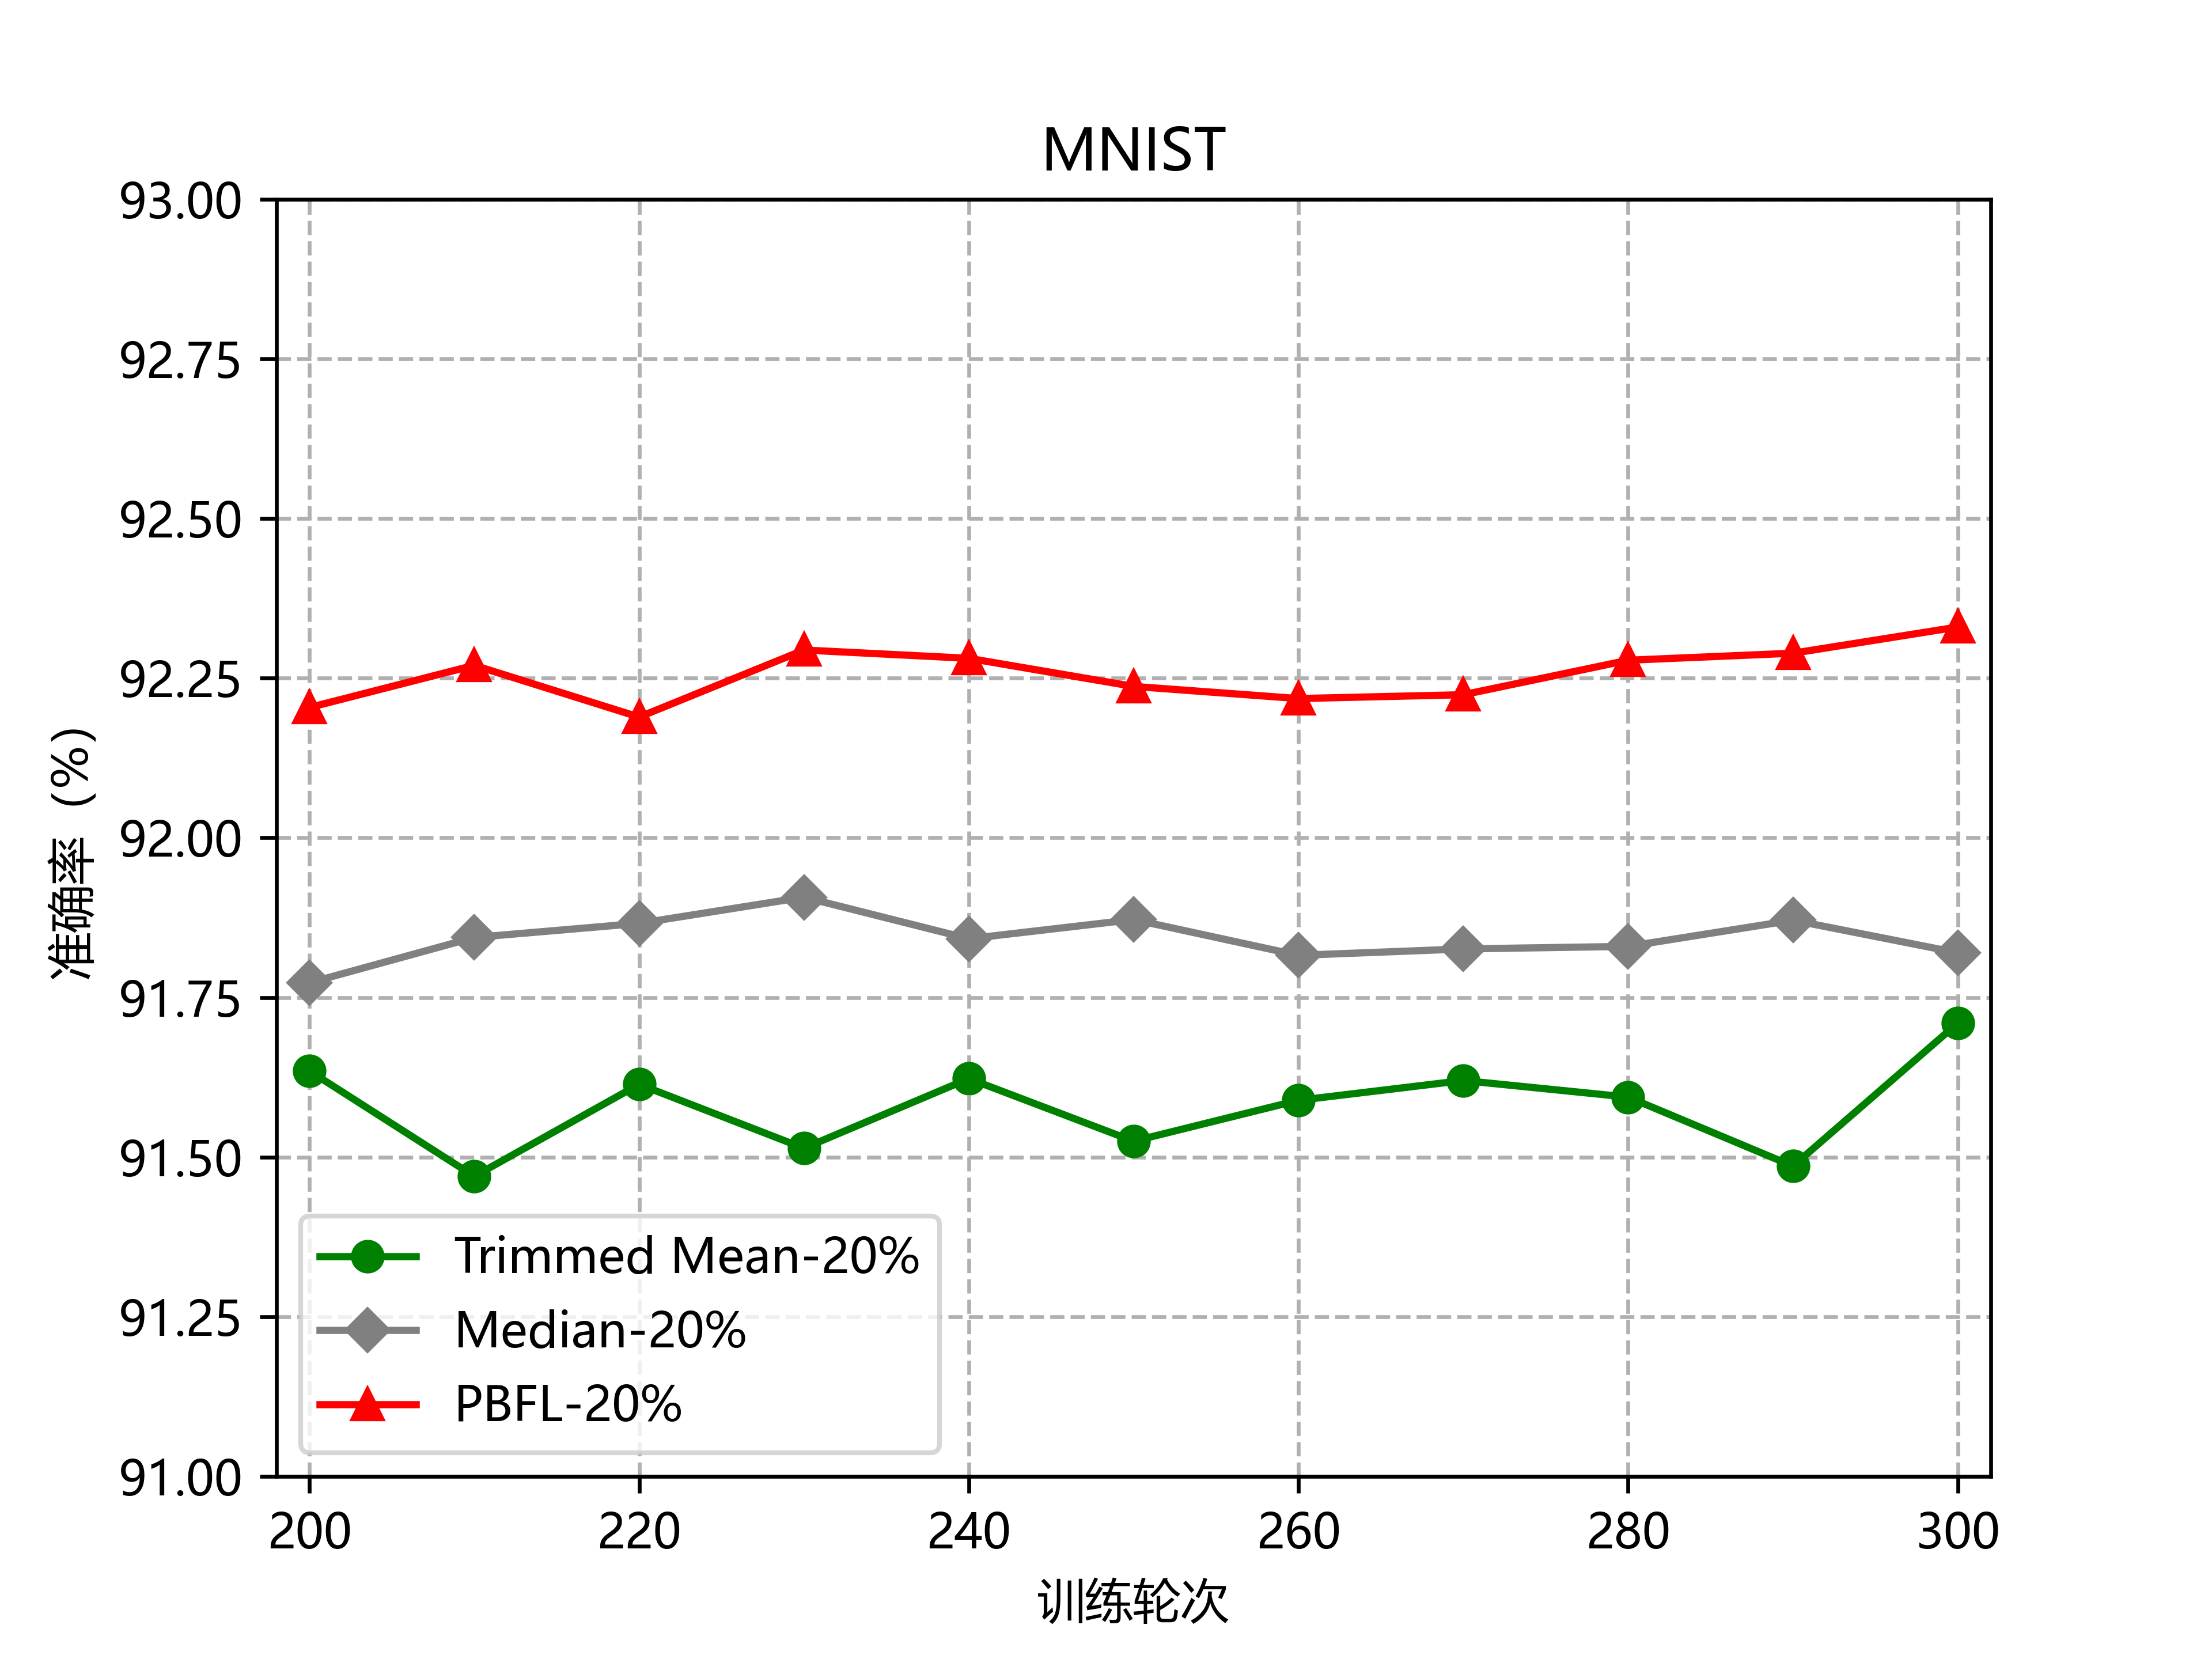
\includegraphics[width=\linewidth]{img/mnist-LF-win-2.png}
		\end{minipage}
	}
%	\hspace{-1.0in}
%	\qquad
	\subfloat[LFA攻击(CIFAR-10)]{
		\begin{minipage}[b]{0.48\textwidth}
			\centering
			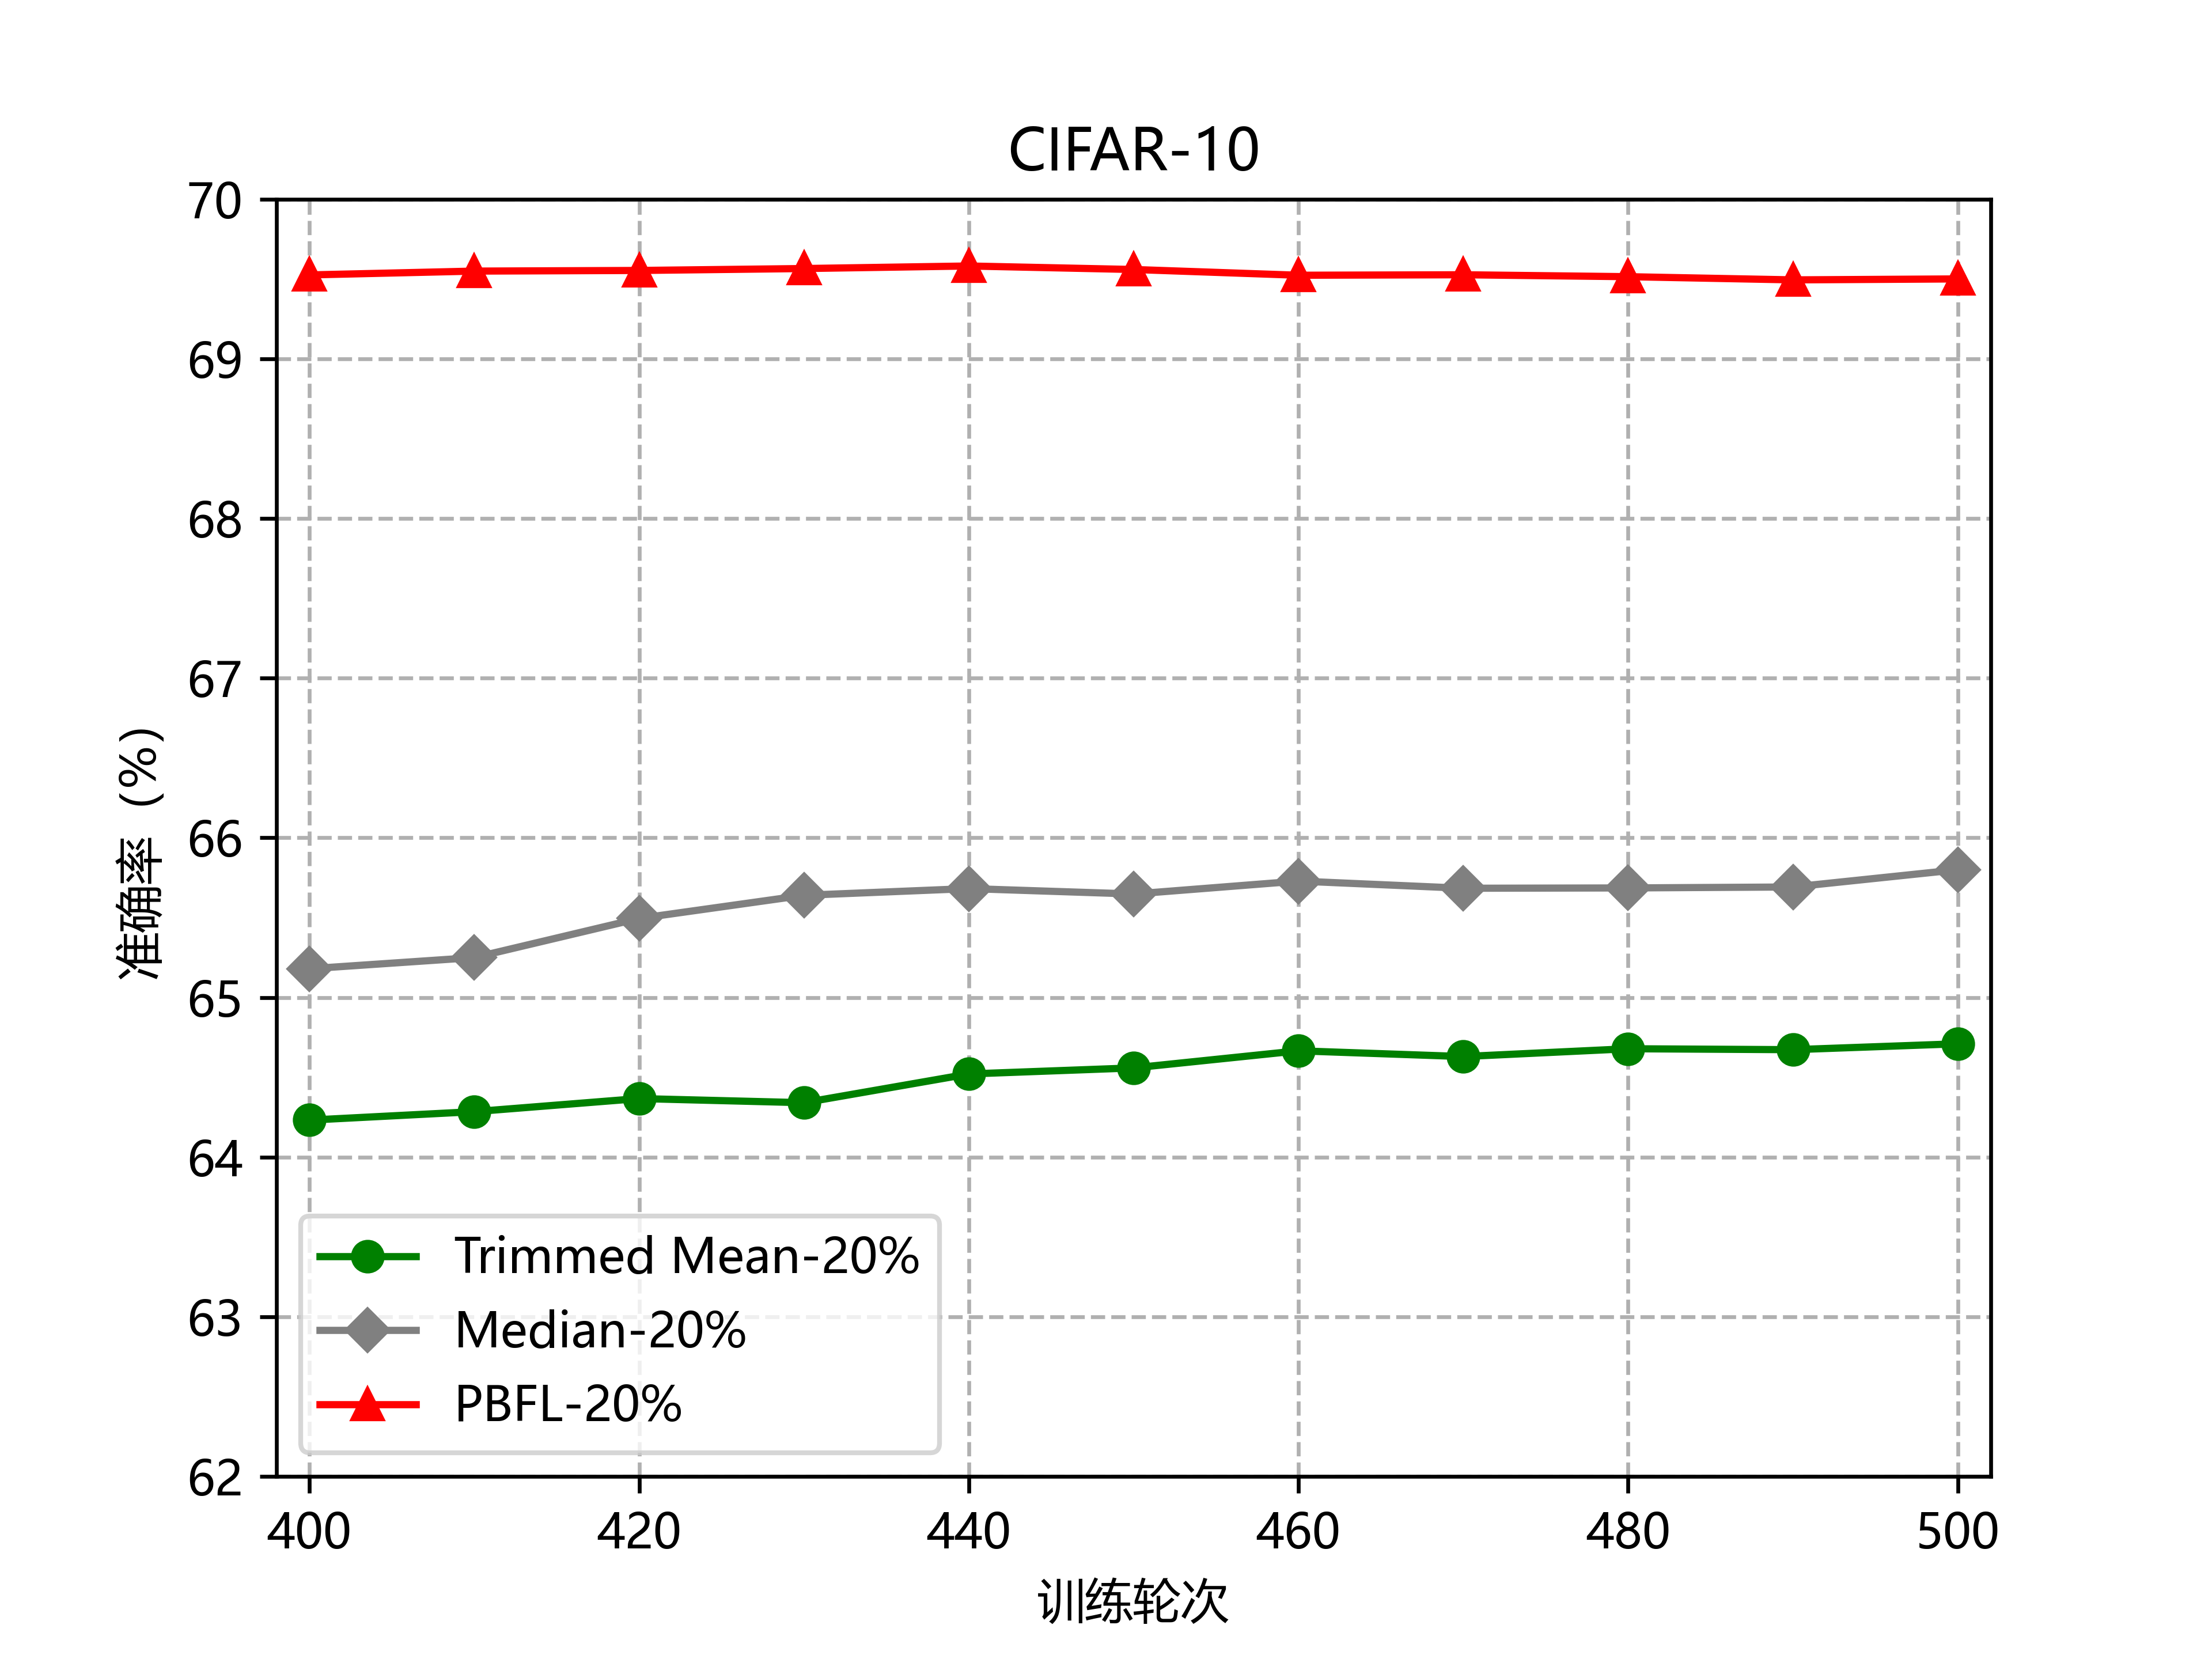
\includegraphics[width=\linewidth]{img/cifar-LF-win-2.png}
		\end{minipage}
	}
	\caption{不同训练轮次对训练准确率的影响}
	\label{f3}
\end{figure}

\textbf{不同GA攻击标准差的影响:}在实施GA攻击时,变换采样随机数的标准差,以此测试不同聚合算法的稳定性。本小节固定拜占庭节点占比为50\%,在表\ref{mnist-std-ga}和表\ref{cifar-std-ga}中给出了不同方法在两种数据集上对不同标准差GA攻击的准确率结果。可以观察到聚合算法Krum、Median、Trimmed Mean以及PBFL都能在不同标准差的GA攻击下完成鲁棒聚合,其中PBFL、Median以及Trimmed Mean准确率表现处在第一梯队。

%\begin{table}[] 
%	\begin{tabular}{llllllllllll} 
%		\multicolumn{6}{c}{MNIST}                                    & \multicolumn{6}{c}{CIFAR10}                                  \\
%		GA攻击标准差 & \multicolumn{5}{l}{不同方法收敛准确率(\%)}                  & GA攻击标准差 & \multicolumn{5}{c}{不同方法收敛准确率(\%)}                  \\
%		& FedAvg & Krum  & Median & Trimmed Mean & PBFL(本方案) &         & FedAvg & Krum  & Median & Trimmed Mean & PBFL(本方案) \\
%		 50      & 50.13  & 85.47 & 91.90  & 91.90        & 91.97     & 50      & 10.00  & 62.17 & 66.83  & 66.48        & 65.45     \\
%		 100     & 50.24  & 86.35 & 91.87  & 91.88        & 91.96     & 100     & 10.00  & 61.68 & 66.18  & 66.50        & 65.77     \\
%		 150     & 50.36  & 85.63 & 91.89  & 91.93        & 91.94     & 150     & 10.00  & 60.99 & 66.32  & 66.49        & 66.34     \\
%		 200     & 50.23  & 86.01 & 91.92  & 91.92        & 91.95     & 200     & 10.00  & 61.27 & 66.44  & 66.56        & 65.83    
%	\end{tabular}
%\end{table}

\begin{table}[]
		\centering 	
		\caption{GA攻击标准差影响(MNIST)}
		\label{mnist-std-ga}
	\begin{tabular}{l|lllll} 
		\toprule \multicolumn{1}{c|}{}         & \multicolumn{5}{c}{不同方法收敛准确率(\%)}                                                                                                      \\ \midrule \multicolumn{1}{c|}{GA攻击标准差} & \multicolumn{1}{l|}{FedAvg} & \multicolumn{1}{l|}{Krum}  & \multicolumn{1}{l|}{Median} & \multicolumn{1}{l|}{Trimmed Mean} & PBFL(本方案) \\ \hline 50                            & \multicolumn{1}{l|}{50.13}  & \multicolumn{1}{l|}{85.47} & \multicolumn{1}{l|}{91.90}  & \multicolumn{1}{l|}{91.90}        & 91.97     \\ \hline 100                           & \multicolumn{1}{l|}{50.24}  & \multicolumn{1}{l|}{86.35} & \multicolumn{1}{l|}{91.87}  & \multicolumn{1}{l|}{91.88}        & 91.96     \\ \hline 150                           & \multicolumn{1}{l|}{50.36}  & \multicolumn{1}{l|}{85.63} & \multicolumn{1}{l|}{91.89}  & \multicolumn{1}{l|}{91.93}        & 91.94     \\ \hline 200                           & \multicolumn{1}{l|}{50.23}  & \multicolumn{1}{l|}{86.01} & \multicolumn{1}{l|}{91.92}  & \multicolumn{1}{l|}{91.92}        & 91.95     \\ \bottomrule 
	\end{tabular}
\end{table}

\begin{table}[] 
	\centering 	 		\caption{GA攻击标准差影响(CIFAR10)} 		\label{cifar-std-ga}
	\begin{tabular}{l|lllll} \toprule \multicolumn{1}{c|}{}         & \multicolumn{5}{c}{不同方法收敛准确率(\%)}                                                                                                      \\ \midrule \multicolumn{1}{c|}{GA攻击标准差} & \multicolumn{1}{l|}{FedAvg} & \multicolumn{1}{l|}{Krum}  & \multicolumn{1}{l|}{Median} & \multicolumn{1}{l|}{Trimmed Mean} & PBFL(本方案) \\ \hline 50                            & \multicolumn{1}{l|}{10.00}  & \multicolumn{1}{l|}{62.17} & \multicolumn{1}{l|}{66.83}  & \multicolumn{1}{l|}{66.48}        & 65.45     \\ \hline 100                           & \multicolumn{1}{l|}{10.00}  & \multicolumn{1}{l|}{61.68} & \multicolumn{1}{l|}{66.18}  & \multicolumn{1}{l|}{66.50}        & 65.77     \\ \hline 150                           & \multicolumn{1}{l|}{10.00}  & \multicolumn{1}{l|}{60.99} & \multicolumn{1}{l|}{66.32}  & \multicolumn{1}{l|}{66.49}        & 66.34     \\ \hline 200                           & \multicolumn{1}{l|}{10.00}  & \multicolumn{1}{l|}{61.27} & \multicolumn{1}{l|}{66.44}  & \multicolumn{1}{l|}{66.56}        & 65.83     \\ \bottomrule \end{tabular} \end{table}

%\begin{table}[] \begin{tabular}{llllll|llllll} \hline \multicolumn{6}{c|}{MNIST}                                                                                                                                                             & \multicolumn{6}{c}{CIFAR10}                                                                                                                                                            \\ \hline \multicolumn{1}{c|}{\multirow{2}{*}{GA攻击标准差}} & \multicolumn{5}{l|}{不同方法收敛准确率(\%)}                                                                                                     & \multicolumn{1}{l|}{\multirow{2}{*}{GA攻击标准差}} & \multicolumn{5}{c}{不同方法收敛准确率(\%)}                                                                                                      \\ \cline{2-6} \cline{8-12}  \multicolumn{1}{c|}{}                         & \multicolumn{1}{l|}{FedAvg} & \multicolumn{1}{l|}{Krum}  & \multicolumn{1}{l|}{Median} & \multicolumn{1}{l|}{Trimmed Mean} & PBFL(本方案) & \multicolumn{1}{l|}{}                         & \multicolumn{1}{l|}{FedAvg} & \multicolumn{1}{l|}{Krum}  & \multicolumn{1}{l|}{Median} & \multicolumn{1}{l|}{Trimmed Mean} & PBFL(本方案) \\ \hline \multicolumn{1}{l|}{50}                       & \multicolumn{1}{l|}{50.13}  & \multicolumn{1}{l|}{85.47} & \multicolumn{1}{l|}{91.90}  & \multicolumn{1}{l|}{91.90}        & 91.97     & \multicolumn{1}{l|}{50}                       & \multicolumn{1}{l|}{10.00}  & \multicolumn{1}{l|}{62.17} & \multicolumn{1}{l|}{66.83}  & \multicolumn{1}{l|}{66.48}        & 65.45     \\ \hline \multicolumn{1}{l|}{100}                      & \multicolumn{1}{l|}{50.24}  & \multicolumn{1}{l|}{86.35} & \multicolumn{1}{l|}{91.87}  & \multicolumn{1}{l|}{91.88}        & 91.96     & \multicolumn{1}{l|}{100}                      & \multicolumn{1}{l|}{10.00}  & \multicolumn{1}{l|}{61.68} & \multicolumn{1}{l|}{66.18}  & \multicolumn{1}{l|}{66.50}        & 65.77     \\ \hline \multicolumn{1}{l|}{150}                      & \multicolumn{1}{l|}{50.36}  & \multicolumn{1}{l|}{85.63} & \multicolumn{1}{l|}{91.89}  & \multicolumn{1}{l|}{91.93}        & 91.94     & \multicolumn{1}{l|}{150}                      & \multicolumn{1}{l|}{10.00}  & \multicolumn{1}{l|}{60.99} & \multicolumn{1}{l|}{66.32}  & \multicolumn{1}{l|}{66.49}        & 66.34     \\ \hline \multicolumn{1}{l|}{200}                      & \multicolumn{1}{l|}{50.23}  & \multicolumn{1}{l|}{86.01} & \multicolumn{1}{l|}{91.92}  & \multicolumn{1}{l|}{91.92}        & 91.95     & \multicolumn{1}{l|}{200}                      & \multicolumn{1}{l|}{10.00}  & \multicolumn{1}{l|}{61.27} & \multicolumn{1}{l|}{66.44}  & \multicolumn{1}{l|}{66.56}        & 65.83     \\ \hline 
%\end{tabular}
%\end{table}

\textbf{密文运算的影响:}PBFL使用的MHE加密方式,基于CKKS全同态加密,其支持浮点数的加密运算,但是会带来一定的舍入误差。
为了弄清楚密文计算中的舍入误差对方案准确率的影响,本小节将聚合方法的明文实现(Plaintext PBFL,Pt-PBFL)和密文实现(PBFL)进行了对比。图\ref{f4}展示了比较结果,可以看出密文实现对比明文实现基本没有准确率的差距。
笔者分析原因是在神经网络的运算中,一定的舍入误差不影响最后的模型准确率,这也证明了CKKS方案非常适合用于神经网络计算中的隐私保护。

\begin{figure}[htb]
	\centering
	% \vspace{-0.2in}
	\subfloat[20\%GA攻击(MNIST)]{
		\begin{minipage}[b]{0.48\textwidth}
			\centering
			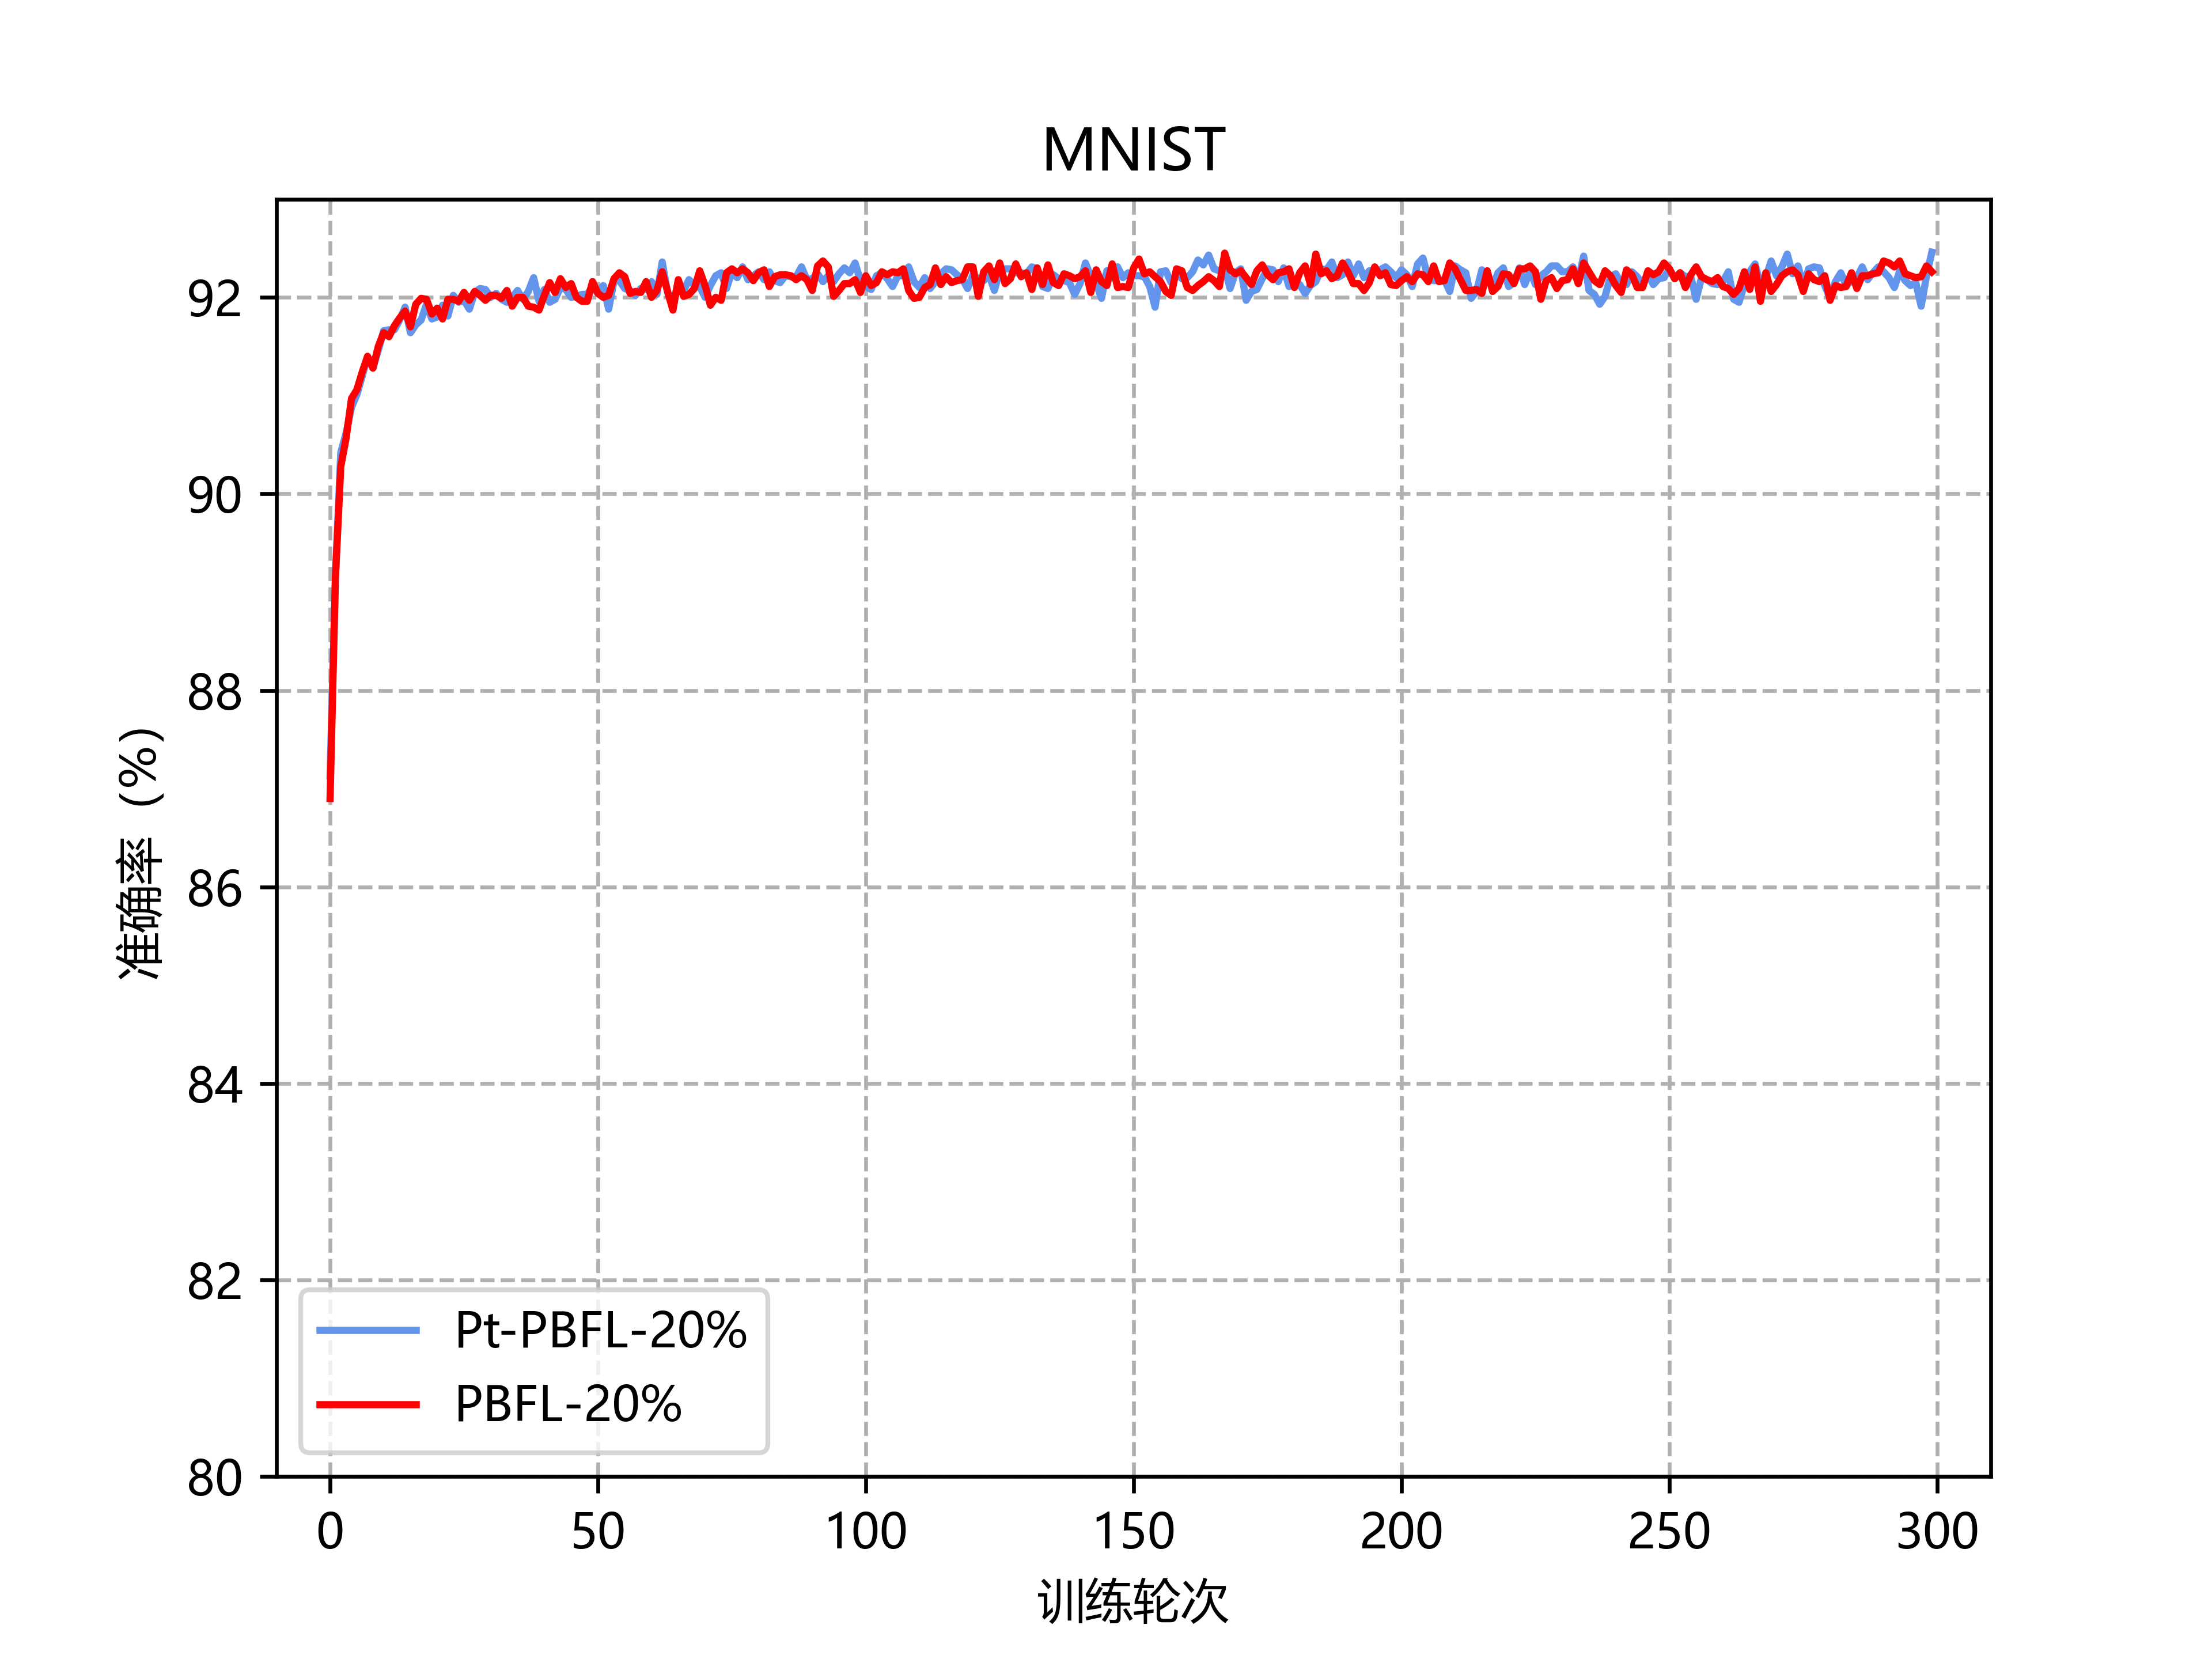
\includegraphics[width=\linewidth]{img/mnist-GA-win20-3.png}
		\end{minipage}
	}
	% \hspace{-1.0in}
	\subfloat[20\%LFA攻击(MNIST)]{
		\begin{minipage}[b]{0.48\textwidth}
			\centering
			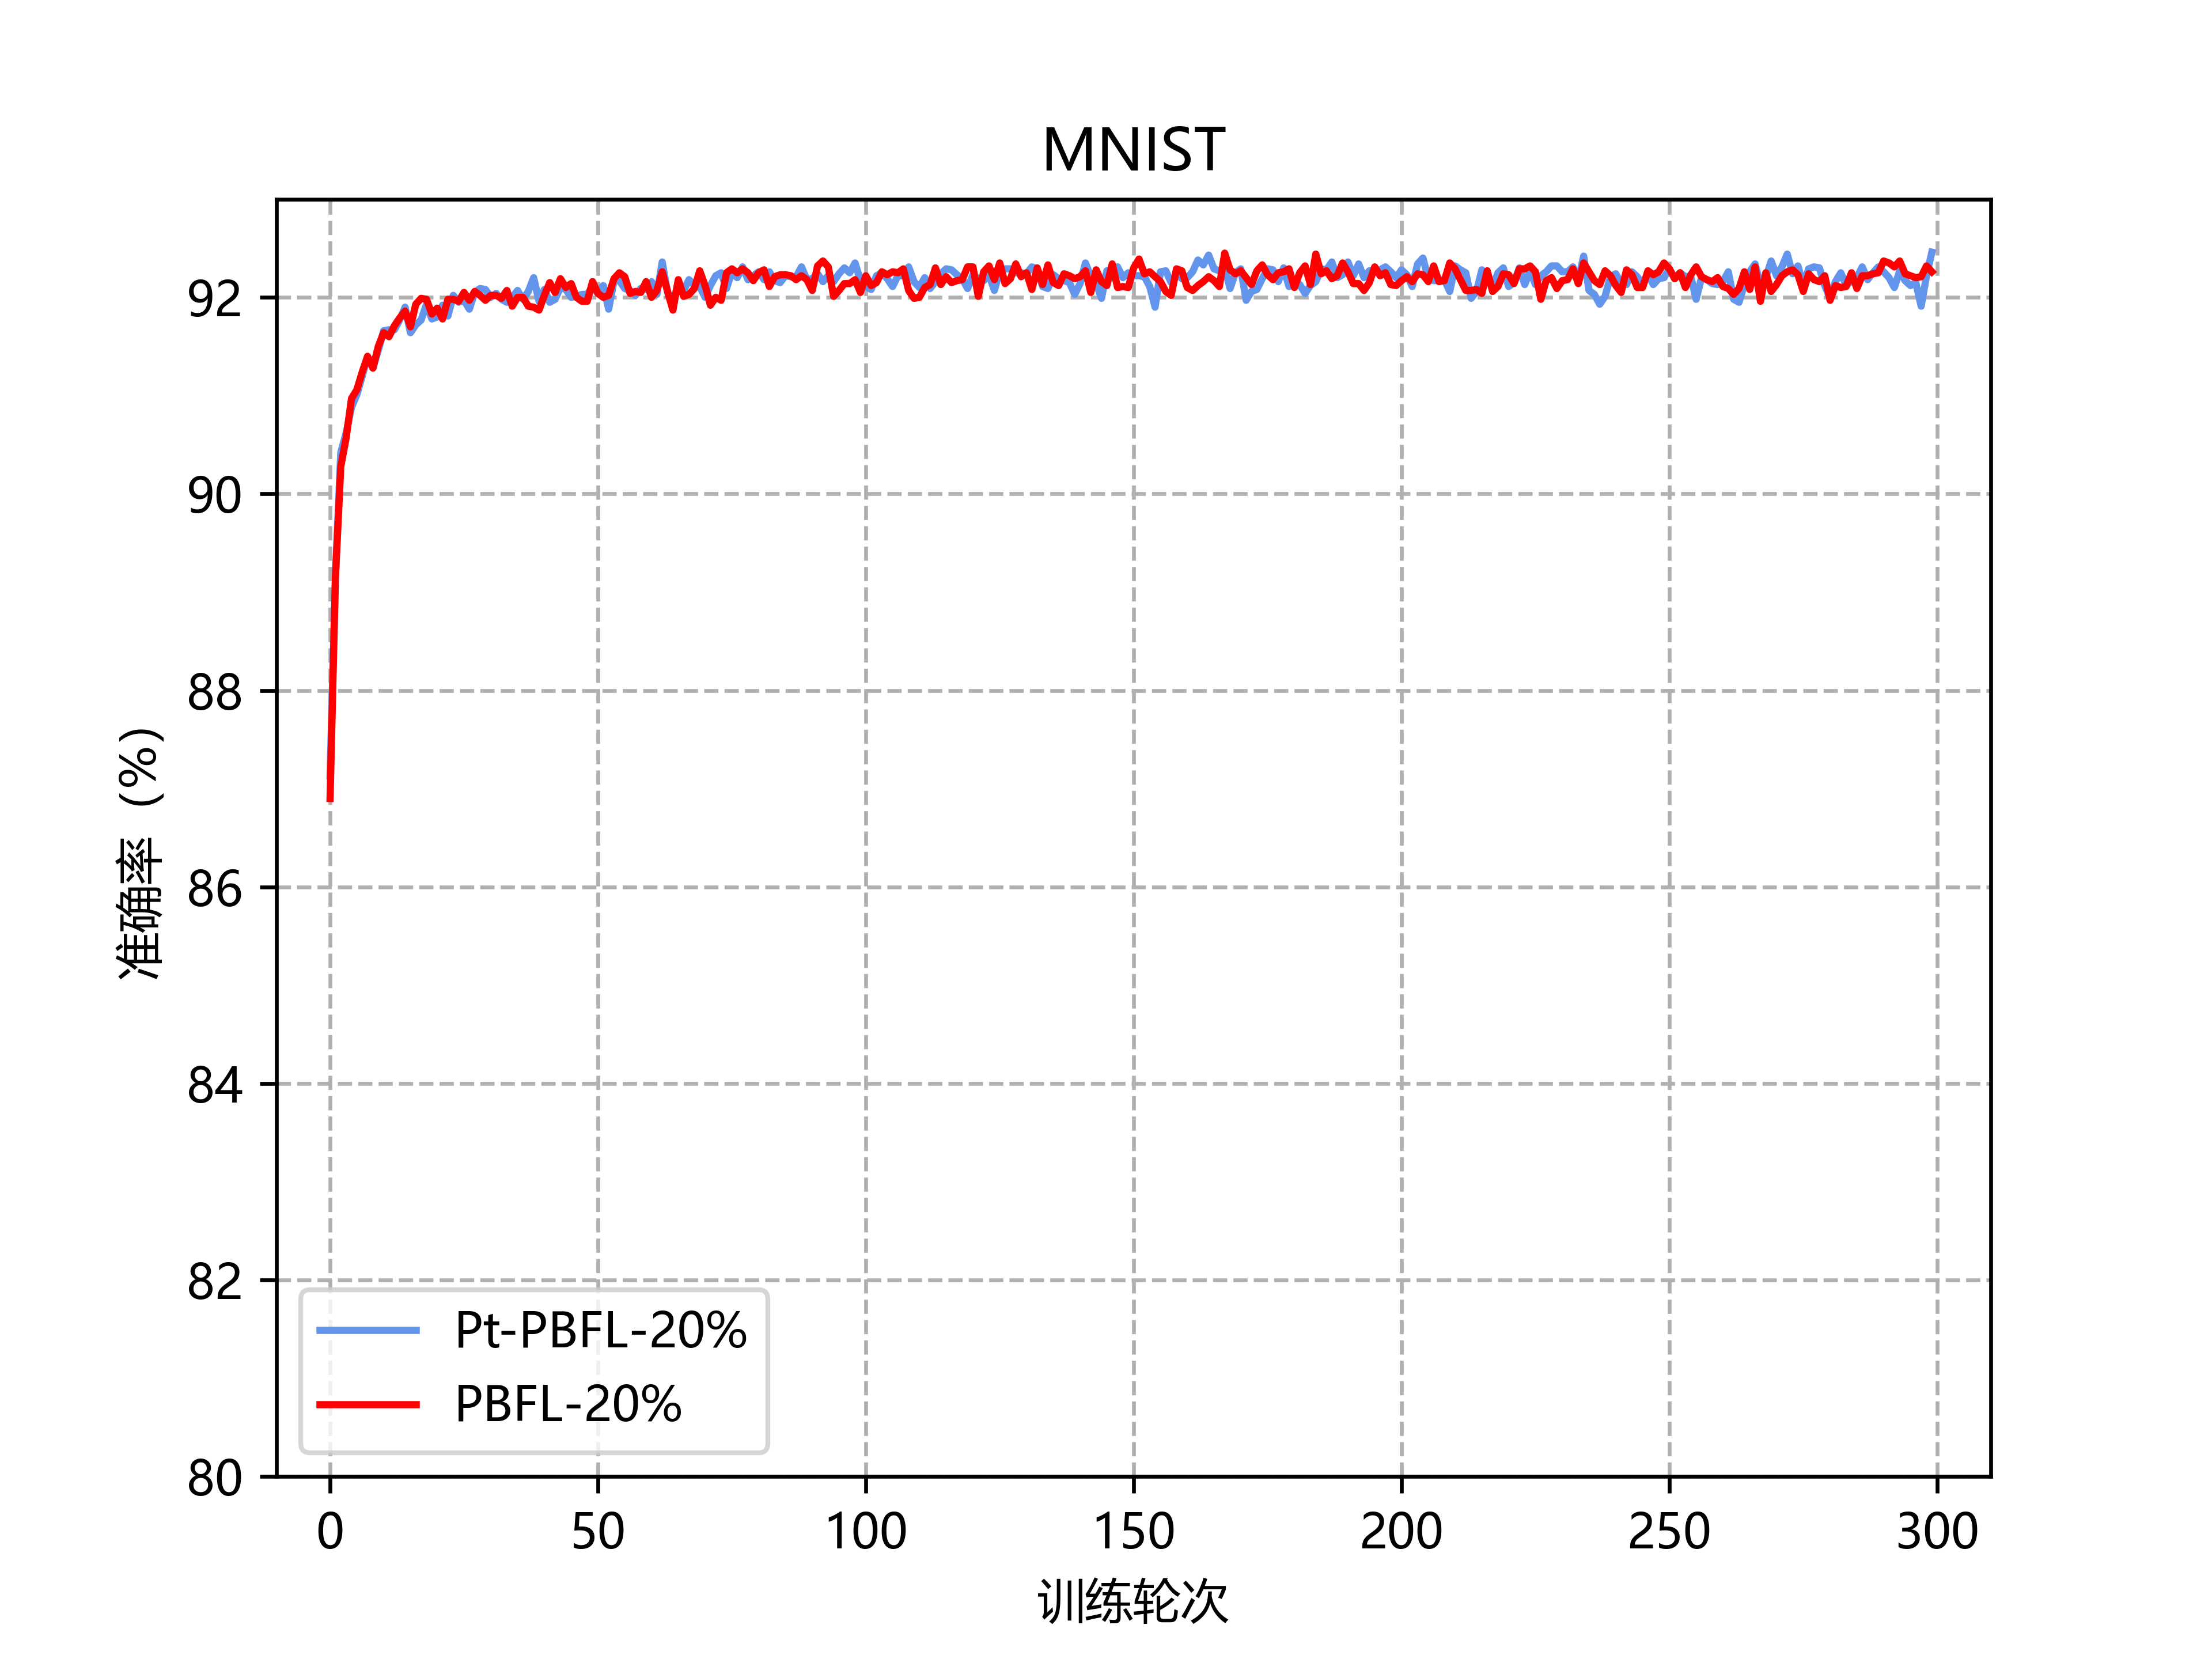
\includegraphics[width=\linewidth]{img/mnist-GA-win20-3.png}
		\end{minipage}
	}
	\caption{PBFL与Pt-PBFL在准确率上的比较}
	\label{f4}
\end{figure}

\subsubsection{聚合权重测试}
%TODO 弄清楚权重表的数据是单个值还是平均值。
从上文的实验结果来看,PBFL在准确性和鲁棒性上,都有一定的优势。
本小节对方案在不同数据集不同攻击方式下,具体的聚合权重分配做了统计,其结果如表\ref{t1}所示。
此时固定拜占庭节点的数量为$30\%$,即51个用户中的15个。结果显示基本上所有的聚合权重都分配给了良性用户,分配给恶意用户的权重可忽略不计。
这也意味着PBFL可以有效的识别恶意用户并降低甚至消除其聚合权重,避免恶意用户干扰的同时,充分利用良性用户上传的参数联合训练,所以PBFL在性能上总体占优。

\begin{table}[htbp]
	% \centering
	\begin{center}
		\caption{PBFL中不同类型节点的聚合权重}
		\label{t1}
		% \resizebox*{\linewidth}{15mm}{
			\scalebox{1}{
				\renewcommand{\arraystretch}{1.2}
				\begin{tabular}{c|c|c|c|c}
					\toprule
					% \hline
					& CIFAR-LF & MNIST-LF & CIFAR-GA & MNIST-GA \\
					\midrule
					良性参与方    & 0.9999   & 0.9988   & 1.0      & 1.0      \\
					\hline
					拜占庭参与方 & 0.0001   & 0.0012   & 0.0      & 0.0      \\
					% \hline
					\bottomrule
			\end{tabular}}
		\end{center}
	\end{table}
%\newpage
\section{本章小结}\label{con}
本章针对模型参数的隐私保护需求和对拜占庭节点的鲁棒性需求,提出了一种面向拜占庭容错的模型参数安全聚合技术(PBFL)。
该方案可以在保证用户数据强隐私的同时,实现对典型非目标性拜占庭攻击的防御。
同时本章对提出的PBFL也提供了详尽的安全性分析和收敛性分析,证明了方案的安全性和收敛性。
除此之外,本章还在真实世界的数据集上做了丰富的对比实验,展现了PBFL在准确率和鲁棒性上的优势。
然而,方案的鲁棒性假设基于用户间数据分布的一致性(IID),对于一些非独立同分布数据(Non-IID)场景的联合训练,PBFL的鲁棒性较弱。
%对于Non-IID数据的隐私鲁棒聚合问题,本文将其作为一个未来的研究方向。
此外,妥协于密文计算的限制和对计算高效的追求,PBFL在面对更加强大敌手时的鲁棒性还有待验证。